% $Header: /cvsroot/latex-beamer/latex-beamer/solutions/generic-talks/generic-ornate-15min-45min.en.tex,v 1.5 2007/01/28 20:48:23 tantau Exp $

\documentclass{beamer}
%\usecolortheme[RGB={205,173,0}]{structure} %Gold
\usecolortheme[RGB={218, 165, 32}]{structure} %Golden Rod
% This file is a solution template for:

% - Giving a talk on some subject.
% - The talk is between 15min and 45min long.
% - Style is ornate.
\usepackage{epstopdf} %put by hand to use .eps files with pdflatex
%\usepackage{longtable}
\usepackage{multirow}
\usepackage{hepparticles}
\usepackage{heppennames}


%%%%%%%%%%%%%%%%%%%%%%%%%%%%%%%%%%%%%%%%%%%%%%%%%%%%%%%%%%%%%%%%%%%%
%
%  Common definitions
%
%  N.B. use of \providecommand rather than \newcommand means
%       that a definition is ignored if already specified
%
%                                              L. Taylor 18 Feb 2005
%%%%%%%%%%%%%%%%%%%%%%%%%%%%%%%%%%%%%%%%%%%%%%%%%%%%%%%%%%%%%%%%%%%%

% Some shorthand
% turn off italics
\providecommand {\etal}{\mbox{et al.}\xspace} %et al. - no preceding comma
\providecommand {\ie}{\mbox{i.e.}\xspace}     %i.e.
\providecommand {\eg}{\mbox{e.g.}\xspace}     %e.g.
\providecommand {\etc}{\mbox{etc.}\xspace}     %etc.
\providecommand {\vs}{\mbox{\sl vs.}\xspace}      %vs.
\providecommand {\mdash}{\ensuremath{\mathrm{-}}} % for use within formulas

% some terms whose definition we may change
\providecommand {\Lone}{Level-1\xspace} % Level-1 or L1 ?
\providecommand {\Ltwo}{Level-2\xspace}
\providecommand {\Lthree}{Level-3\xspace}

% Some software programs (alphabetized)
\providecommand{\ACERMC} {\textsc{AcerMC}\xspace}
\providecommand{\ALPGEN} {{\textsc{alpgen}}\xspace}
\providecommand{\CHARYBDIS} {{\textsc{charybdis}}\xspace}
\providecommand{\CMKIN} {\textsc{cmkin}\xspace}
\providecommand{\CMSIM} {{\textsc{cmsim}}\xspace}
\providecommand{\CMSSW} {{\textsc{cmssw}}\xspace}
\providecommand{\COBRA} {{\textsc{cobra}}\xspace}
\providecommand{\COCOA} {{\textsc{cocoa}}\xspace}
\providecommand{\COMPHEP} {\textsc{CompHEP}\xspace}
\providecommand{\EVTGEN} {{\textsc{evtgen}}\xspace}
\providecommand{\FAMOS} {{\textsc{famos}}\xspace}
\providecommand{\GARCON} {\textsc{garcon}\xspace}
\providecommand{\GARFIELD} {{\textsc{garfield}}\xspace}
\providecommand{\GEANE} {{\textsc{geane}}\xspace}
\providecommand{\GEANTfour} {{\textsc{geant4}}\xspace}
\providecommand{\GEANTthree} {{\textsc{geant3}}\xspace}
\providecommand{\GEANT} {{\textsc{geant}}\xspace}
\providecommand{\HDECAY} {\textsc{hdecay}\xspace}
\providecommand{\HERWIG} {{\textsc{herwig}}\xspace}
\providecommand{\HIGLU} {{\textsc{higlu}}\xspace}
\providecommand{\HIJING} {{\textsc{hijing}}\xspace}
\providecommand{\IGUANA} {\textsc{iguana}\xspace}
\providecommand{\ISAJET} {{\textsc{isajet}}\xspace}
\providecommand{\ISAPYTHIA} {{\textsc{isapythia}}\xspace}
\providecommand{\ISASUGRA} {{\textsc{isasugra}}\xspace}
\providecommand{\ISASUSY} {{\textsc{isasusy}}\xspace}
\providecommand{\ISAWIG} {{\textsc{isawig}}\xspace}
\providecommand{\MADGRAPH} {\textsc{MadGraph}\xspace}
\providecommand{\MCATNLO} {\textsc{mc@nlo}\xspace}
\providecommand{\MCFM} {\textsc{mcfm}\xspace}
\providecommand{\MILLEPEDE} {{\textsc{millepede}}\xspace}
\providecommand{\ORCA} {{\textsc{orca}}\xspace}
\providecommand{\OSCAR} {{\textsc{oscar}}\xspace}
\providecommand{\PHOTOS} {\textsc{photos}\xspace}
\providecommand{\PROSPINO} {\textsc{prospino}\xspace}
\providecommand{\PYTHIA} {{\textsc{pythia}}\xspace}
\providecommand{\SHERPA} {{\textsc{sherpa}}\xspace}
\providecommand{\TAUOLA} {\textsc{tauola}\xspace}
\providecommand{\TOPREX} {\textsc{TopReX}\xspace}
\providecommand{\XDAQ} {{\textsc{xdaq}}\xspace}


%  Experiments
\providecommand {\DZERO}{D\O\xspace}     %etc.


% Measurements and units...

\providecommand{\de}{\ensuremath{^\circ}}
\providecommand{\ten}[1]{\ensuremath{\times \text{10}^\text{#1}}}
\providecommand{\unit}[1]{\ensuremath{\text{\,#1}}\xspace}
\providecommand{\mum}{\ensuremath{\,\mu\text{m}}\xspace}
\providecommand{\micron}{\ensuremath{\,\mu\text{m}}\xspace}
\providecommand{\cm}{\ensuremath{\,\text{cm}}\xspace}
\providecommand{\mm}{\ensuremath{\,\text{mm}}\xspace}
\providecommand{\mus}{\ensuremath{\,\mu\text{s}}\xspace}
\providecommand{\keV}{\ensuremath{\,\text{ke\hspace{-.08em}V}}\xspace}
\providecommand{\MeV}{\ensuremath{\,\text{Me\hspace{-.08em}V}}\xspace}
\providecommand{\GeV}{\ensuremath{\,\text{Ge\hspace{-.08em}V}}\xspace}
\providecommand{\gev}{\GeV}
\providecommand{\TeV}{\ensuremath{\,\text{Te\hspace{-.08em}V}}\xspace}
\providecommand{\PeV}{\ensuremath{\,\text{Pe\hspace{-.08em}V}}\xspace}
\providecommand{\keVc}{\ensuremath{{\,\text{ke\hspace{-.08em}V\hspace{-0.16em}/\hspace{-0.08em}}c}}\xspace}
\providecommand{\MeVc}{\ensuremath{{\,\text{Me\hspace{-.08em}V\hspace{-0.16em}/\hspace{-0.08em}}c}}\xspace}
\providecommand{\GeVc}{\ensuremath{{\,\text{Ge\hspace{-.08em}V\hspace{-0.16em}/\hspace{-0.08em}}c}}\xspace}
\providecommand{\TeVc}{\ensuremath{{\,\text{Te\hspace{-.08em}V\hspace{-0.16em}/\hspace{-0.08em}}c}}\xspace}
\providecommand{\keVcc}{\ensuremath{{\,\text{ke\hspace{-.08em}V\hspace{-0.16em}/\hspace{-0.08em}}c^\text{2}}}\xspace}
\providecommand{\MeVcc}{\ensuremath{{\,\text{Me\hspace{-.08em}V\hspace{-0.16em}/\hspace{-0.08em}}c^\text{2}}}\xspace}
%\providecommand{\GeVcc}{\ensuremath{{\,\text{Ge\hspace{-.08em}V\hspace{-0.16em}/\hspace{-0.08em}}c^\text{2}}}\xspace}
\providecommand{\GeVcc}{\GeV}
\providecommand{\TeVcc}{\ensuremath{{\,\text{Te\hspace{-.08em}V\hspace{-0.16em}/\hspace{-0.08em}}c^\text{2}}}\xspace}

\providecommand{\pbinv} {\mbox{\ensuremath{\,\text{pb}^\text{$-$1}}}\xspace}
\providecommand{\fbinv} {\mbox{\ensuremath{\,\text{fb}^\text{$-$1}}}\xspace}
\providecommand{\nbinv} {\mbox{\ensuremath{\,\text{nb}^\text{$-$1}}}\xspace}
\providecommand{\percms}{\ensuremath{\,\text{cm}^\text{$-$2}\,\text{s}^\text{$-$1}}\xspace}
\providecommand{\lumi}{\ensuremath{\mathcal{L}}\xspace}
\providecommand{\Lumi}{\ensuremath{\mathcal{L}}\xspace}%both upper and lower
%
% Need a convention here:
\providecommand{\LvLow}  {\ensuremath{\mathcal{L}=\text{10}^\text{32}\,\text{cm}^\text{$-$2}\,\text{s}^\text{$-$1}}\xspace}
\providecommand{\LLow}   {\ensuremath{\mathcal{L}=\text{10}^\text{33}\,\text{cm}^\text{$-$2}\,\text{s}^\text{$-$1}}\xspace}
\providecommand{\lowlumi}{\ensuremath{\mathcal{L}=\text{2}\times \text{10}^\text{33}\,\text{cm}^\text{$-$2}\,\text{s}^\text{$-$1}}\xspace}
\providecommand{\LMed}   {\ensuremath{\mathcal{L}=\text{2}\times \text{10}^\text{33}\,\text{cm}^\text{$-$2}\,\text{s}^\text{$-$1}}\xspace}
\providecommand{\LHigh}  {\ensuremath{\mathcal{L}=\text{10}^\text{34}\,\text{cm}^\text{$-$2}\,\text{s}^\text{$-$1}}\xspace}
\providecommand{\hilumi} {\ensuremath{\mathcal{L}=\text{10}^\text{34}\,\text{cm}^\text{$-$2}\,\text{s}^\text{$-$1}}\xspace}

% Physics symbols ...

\providecommand{\PT}{\ensuremath{p_{\mathrm{T}}}\xspace}
\providecommand{\pt}{\ensuremath{p_{\mathrm{T}}}\xspace}
\providecommand{\ET}{\ensuremath{E_{\mathrm{T}}}\xspace}
\providecommand{\HT}{\ensuremath{H_{\mathrm{T}}}\xspace}
\providecommand{\et}{\ensuremath{E_{\mathrm{T}}}\xspace}
\providecommand{\Em}{\ensuremath{E\hspace{-0.6em}/}\xspace}
\providecommand{\Pm}{\ensuremath{p\hspace{-0.5em}/}\xspace}
\providecommand{\PTm}{\ensuremath{{p}_\mathrm{T}\hspace{-1.02em}/}\xspace}
\providecommand{\PTslash}{\ensuremath{{p}_\mathrm{T}\hspace{-1.02em}/}\xspace}
\providecommand{\ETm}{\ensuremath{E_{\mathrm{T}}^{\text{miss}}}\xspace}
\providecommand{\MET}{\ETm}
\providecommand{\ETmiss}{\ETm}
\providecommand{\ETslash}{\ensuremath{E_{\mathrm{T}}\hspace{-1.1em}/}\xspace}
\providecommand{\VEtmiss}{\ensuremath{{\vec E}_{\mathrm{T}}^{\text{miss}}}\xspace}

% roman face derivative
\providecommand{\dd}[2]{\ensuremath{\frac{\mathrm{d} #1}{\mathrm{d} #2}}}
\providecommand{\ddinline}[2]{\ensuremath{\mathrm{d} #1/\mathrm{d} #2}}



%\ifthenelse{\boolean{cms@italic}}{\providecommand{\cmsSymbolFace}{\relax}}{\providecommand{\cmsSymbolFace}{\mathrm}}

% Particle names which track the italic/non-italic face convention
\providecommand{\zp}{\ensuremath{\cmsSymbolFace{Z}^\prime}\xspace}
\providecommand{\JPsi}{\ensuremath{\cmsSymbolFace{J}\hspace{-.08em}/\hspace{-.14em}\psi}\xspace}
\providecommand{\Z}{\ensuremath{\cmsSymbolFace{Z}}\xspace}
%%%%%%%%%%%%%\providecommand{\ttbar}{\ensuremath{\cmsSymbolFace{t}\overline{\cmsSymbolFace{t}}}\xspace}

% Extensions for missing names in PENNAMES
% Extensions for missing names in PENNAMES % note no xspace, to match syntax in PENNAMES
\providecommand{\cPgn}{\ensuremath{\nu}} % generic neutrino
\providecommand{\cPJgy}{\ensuremath{\cmsSymbolFace{J}\hspace{-.08em}/\hspace{-.14em}\psi}} % J/Psi (no mass)
\providecommand{\cPZ}{\ensuremath{\cmsSymbolFace{Z}}} % plain Z (no superscript 0)
\providecommand{\cPZpr}{\ensuremath{\cmsSymbolFace{Z}^\prime}} % plain Z'
\providecommand{\cPqb}{\ensuremath{\cmsSymbolFace{b}}} % b for b quark
\providecommand{\cPqt}{\ensuremath{\cmsSymbolFace{t}}} % t for t quark
\providecommand{\cPqc}{\ensuremath{\cmsSymbolFace{c}}} % c for c quark
\providecommand{\cPaqb}{\ensuremath{\overline{\cmsSymbolFace{b}}}} % b for b anti-quark
\providecommand{\cPaqt}{\ensuremath{\overline{\cmsSymbolFace{t}}}} % t for t anti-quark
\providecommand{\cPaqc}{\ensuremath{\overline{\cmsSymbolFace{c}}}} % c for c anti-quark

% SM (still to be classified)

\providecommand{\AFB}{\ensuremath{A_\text{FB}}\xspace}
\providecommand{\wangle}{\ensuremath{\sin^{2}\theta_{\text{eff}}^\text{lept}(M^2_\Z)}\xspace}
\providecommand{\stat}{\ensuremath{\,\text{(stat.)}}\xspace}
\providecommand{\syst}{\ensuremath{\,\text{(syst.)}}\xspace}
\providecommand{\kt}{\ensuremath{k_{\mathrm{T}}}\xspace}

\providecommand{\BC}{\ensuremath{\mathrm{B_{c}}}\xspace}
\providecommand{\bbarc}{\ensuremath{\mathrm{\overline{b}c}}\xspace}
\providecommand{\bbbar}{\ensuremath{\mathrm{b\overline{b}}}\xspace}
\providecommand{\ccbar}{\ensuremath{\mathrm{c\overline{c}}}\xspace}
\providecommand{\bspsiphi}{\ensuremath{\mathrm{B_s} \to \JPsi\, \phi}\xspace}
\providecommand{\EE}{\ensuremath{\mathrm{e^+e^-}}\xspace}
\providecommand{\MM}{\ensuremath{\mu^+\mu^-}\xspace}
\providecommand{\TT}{\ensuremath{\tau^+\tau^-}\xspace}

%%%  E-gamma definitions
\providecommand{\HGG}{\ensuremath{\mathrm{H}\to\gamma\gamma}}
\providecommand{\GAMJET}{\ensuremath{\gamma + \text{jet}}}
\providecommand{\PPTOJETS}{\ensuremath{\mathrm{pp}\to\text{jets}}}
\providecommand{\PPTOGG}{\ensuremath{\mathrm{pp}\to\gamma\gamma}}
\providecommand{\PPTOGAMJET}{\ensuremath{\mathrm{pp}\to\gamma + \mathrm{jet}}}
\providecommand{\MH}{\ensuremath{m_{\mathrm{H}}}}
\providecommand{\RNINE}{\ensuremath{R_\mathrm{9}}}
\providecommand{\DR}{\ensuremath{\Delta R}}





%%%%%%
% From Albert
%

\providecommand{\ga}{\ensuremath{\gtrsim}}
\providecommand{\la}{\ensuremath{\lesssim}}
%
\providecommand{\swsq}{\ensuremath{\sin^2\theta_\cmsSymbolFace{W}}\xspace}
\providecommand{\cwsq}{\ensuremath{\cos^2\theta_\cmsSymbolFace{W}}\xspace}
\providecommand{\tanb}{\ensuremath{\tan\beta}\xspace}
\providecommand{\tanbsq}{\ensuremath{\tan^{2}\beta}\xspace}
\providecommand{\sidb}{\ensuremath{\sin 2\beta}\xspace}
\providecommand{\alpS}{\ensuremath{\alpha_S}\xspace}
\providecommand{\alpt}{\ensuremath{\tilde{\alpha}}\xspace}

\providecommand{\QL}{\ensuremath{\cmsSymbolFace{Q}_\cmsSymbolFace{L}}\xspace}
\providecommand{\sQ}{\ensuremath{\tilde{\cmsSymbolFace{Q}}}\xspace}
\providecommand{\sQL}{\ensuremath{\tilde{\cmsSymbolFace{Q}}_\cmsSymbolFace{L}}\xspace}
\providecommand{\ULC}{\ensuremath{\cmsSymbolFace{U}_\cmsSymbolFace{L}^\cmsSymbolFace{C}}\xspace}
\providecommand{\sUC}{\ensuremath{\tilde{\cmsSymbolFace{U}}^\cmsSymbolFace{C}}\xspace}
\providecommand{\sULC}{\ensuremath{\tilde{\cmsSymbolFace{U}}_\cmsSymbolFace{L}^\cmsSymbolFace{C}}\xspace}
\providecommand{\DLC}{\ensuremath{\cmsSymbolFace{D}_\cmsSymbolFace{L}^\cmsSymbolFace{C}}\xspace}
\providecommand{\sDC}{\ensuremath{\tilde{\cmsSymbolFace{D}}^\cmsSymbolFace{C}}\xspace}
\providecommand{\sDLC}{\ensuremath{\tilde{\cmsSymbolFace{D}}_\cmsSymbolFace{L}^\cmsSymbolFace{C}}\xspace}
\providecommand{\LL}{\ensuremath{\cmsSymbolFace{L}_\cmsSymbolFace{L}}\xspace}
\providecommand{\sL}{\ensuremath{\tilde{\cmsSymbolFace{L}}}\xspace}
\providecommand{\sLL}{\ensuremath{\tilde{\cmsSymbolFace{L}}_\cmsSymbolFace{L}}\xspace}
\providecommand{\ELC}{\ensuremath{\cmsSymbolFace{E}_\cmsSymbolFace{L}^\cmsSymbolFace{C}}\xspace}
\providecommand{\sEC}{\ensuremath{\tilde{\cmsSymbolFace{E}}^\cmsSymbolFace{C}}\xspace}
\providecommand{\sELC}{\ensuremath{\tilde{\cmsSymbolFace{E}}_\cmsSymbolFace{L}^\cmsSymbolFace{C}}\xspace}
\providecommand{\sEL}{\ensuremath{\tilde{\cmsSymbolFace{E}}_\cmsSymbolFace{L}}\xspace}
\providecommand{\sER}{\ensuremath{\tilde{\cmsSymbolFace{E}}_\cmsSymbolFace{R}}\xspace}
\providecommand{\sFer}{\ensuremath{\tilde{\cmsSymbolFace{f}}}\xspace}
\providecommand{\sQua}{\ensuremath{\tilde{\cmsSymbolFace{q}}}\xspace}
\providecommand{\sUp}{\ensuremath{\tilde{\cmsSymbolFace{u}}}\xspace}
\providecommand{\suL}{\ensuremath{\tilde{\cmsSymbolFace{u}}_\cmsSymbolFace{L}}\xspace}
\providecommand{\suR}{\ensuremath{\tilde{\cmsSymbolFace{u}}_\cmsSymbolFace{R}}\xspace}
\providecommand{\sDw}{\ensuremath{\tilde{\cmsSymbolFace{d}}}\xspace}
\providecommand{\sdL}{\ensuremath{\tilde{\cmsSymbolFace{d}}_\cmsSymbolFace{L}}\xspace}
\providecommand{\sdR}{\ensuremath{\tilde{\cmsSymbolFace{d}}_\cmsSymbolFace{R}}\xspace}
\providecommand{\sTop}{\ensuremath{\tilde{\cmsSymbolFace{t}}}\xspace}
\providecommand{\stL}{\ensuremath{\tilde{\cmsSymbolFace{t}}_\cmsSymbolFace{L}}\xspace}
\providecommand{\stR}{\ensuremath{\tilde{\cmsSymbolFace{t}}_\cmsSymbolFace{R}}\xspace}
\providecommand{\stone}{\ensuremath{\tilde{\cmsSymbolFace{t}}_1}\xspace}
\providecommand{\sttwo}{\ensuremath{\tilde{\cmsSymbolFace{t}}_2}\xspace}
\providecommand{\sBot}{\ensuremath{\tilde{\cmsSymbolFace{b}}}\xspace}
\providecommand{\sbL}{\ensuremath{\tilde{\cmsSymbolFace{b}}_\cmsSymbolFace{L}}\xspace}
\providecommand{\sbR}{\ensuremath{\tilde{\cmsSymbolFace{b}}_\cmsSymbolFace{R}}\xspace}
\providecommand{\sbone}{\ensuremath{\tilde{\cmsSymbolFace{b}}_1}\xspace}
\providecommand{\sbtwo}{\ensuremath{\tilde{\cmsSymbolFace{b}}_2}\xspace}
\providecommand{\sLep}{\ensuremath{\tilde{\cmsSymbolFace{l}}}\xspace}
\providecommand{\sLepC}{\ensuremath{\tilde{\cmsSymbolFace{l}}^\cmsSymbolFace{C}}\xspace}
\providecommand{\sEl}{\ensuremath{\tilde{\cmsSymbolFace{e}}}\xspace}
\providecommand{\sElC}{\ensuremath{\tilde{\cmsSymbolFace{e}}^\cmsSymbolFace{C}}\xspace}
\providecommand{\seL}{\ensuremath{\tilde{\cmsSymbolFace{e}}_\cmsSymbolFace{L}}\xspace}
\providecommand{\seR}{\ensuremath{\tilde{\cmsSymbolFace{e}}_\cmsSymbolFace{R}}\xspace}
\providecommand{\snL}{\ensuremath{\tilde{\nu}_L}\xspace}
\providecommand{\sMu}{\ensuremath{\tilde{\mu}}\xspace}
\providecommand{\sNu}{\ensuremath{\tilde{\nu}}\xspace}
\providecommand{\sTau}{\ensuremath{\tilde{\tau}}\xspace}
\providecommand{\Glu}{\ensuremath{\cmsSymbolFace{g}}\xspace}
\providecommand{\sGlu}{\ensuremath{\tilde{\cmsSymbolFace{g}}}\xspace}
\providecommand{\Wpm}{\ensuremath{\cmsSymbolFace{W}^{\pm}}\xspace}
\providecommand{\sWpm}{\ensuremath{\tilde{\cmsSymbolFace{W}}^{\pm}}\xspace}
\providecommand{\Wz}{\ensuremath{\cmsSymbolFace{W}^{0}}\xspace}
\providecommand{\sWz}{\ensuremath{\tilde{\cmsSymbolFace{W}}^{0}}\xspace}
\providecommand{\sWino}{\ensuremath{\tilde{\cmsSymbolFace{W}}}\xspace}
\providecommand{\Bz}{\ensuremath{\cmsSymbolFace{B}^{0}}\xspace}
\providecommand{\sBz}{\ensuremath{\tilde{\cmsSymbolFace{B}}^{0}}\xspace}
\providecommand{\sBino}{\ensuremath{\tilde{\cmsSymbolFace{B}}}\xspace}
\providecommand{\Zz}{\ensuremath{\cmsSymbolFace{Z}^{0}}\xspace}
\providecommand{\sZino}{\ensuremath{\tilde{\cmsSymbolFace{Z}}^{0}}\xspace}
\providecommand{\sGam}{\ensuremath{\tilde{\gamma}}\xspace}
\providecommand{\chiz}{\ensuremath{\tilde{\chi}^{0}}\xspace}
\providecommand{\chip}{\ensuremath{\tilde{\chi}^{+}}\xspace}
\providecommand{\chim}{\ensuremath{\tilde{\chi}^{-}}\xspace}
\providecommand{\chipm}{\ensuremath{\tilde{\chi}^{\pm}}\xspace}
\providecommand{\Hone}{\ensuremath{\cmsSymbolFace{H}_\cmsSymbolFace{d}}\xspace}
\providecommand{\sHone}{\ensuremath{\tilde{\cmsSymbolFace{H}}_\cmsSymbolFace{d}}\xspace}
\providecommand{\Htwo}{\ensuremath{\cmsSymbolFace{H}_\cmsSymbolFace{u}}\xspace}
\providecommand{\sHtwo}{\ensuremath{\tilde{\cmsSymbolFace{H}}_\cmsSymbolFace{u}}\xspace}
\providecommand{\sHig}{\ensuremath{\tilde{\cmsSymbolFace{H}}}\xspace}
\providecommand{\sHa}{\ensuremath{\tilde{\cmsSymbolFace{H}}_\cmsSymbolFace{a}}\xspace}
\providecommand{\sHb}{\ensuremath{\tilde{\cmsSymbolFace{H}}_\cmsSymbolFace{b}}\xspace}
\providecommand{\sHpm}{\ensuremath{\tilde{\cmsSymbolFace{H}}^{\pm}}\xspace}
\providecommand{\hz}{\ensuremath{\cmsSymbolFace{h}^{0}}\xspace}
\providecommand{\Hz}{\ensuremath{\cmsSymbolFace{H}^{0}}\xspace}
\providecommand{\Az}{\ensuremath{\cmsSymbolFace{A}^{0}}\xspace}
\providecommand{\Hpm}{\ensuremath{\cmsSymbolFace{H}^{\pm}}\xspace}
\providecommand{\sGra}{\ensuremath{\tilde{\cmsSymbolFace{G}}}\xspace}
%
\providecommand{\mtil}{\ensuremath{\tilde{m}}\xspace}
%
\providecommand{\rpv}{\ensuremath{\rlap{\kern.2em/}R}\xspace}
\providecommand{\LLE}{\ensuremath{LL\bar{E}}\xspace}
\providecommand{\LQD}{\ensuremath{LQ\bar{D}}\xspace}
\providecommand{\UDD}{\ensuremath{\overline{UDD}}\xspace}
\providecommand{\Lam}{\ensuremath{\lambda}\xspace}
\providecommand{\Lamp}{\ensuremath{\lambda'}\xspace}
\providecommand{\Lampp}{\ensuremath{\lambda''}\xspace}
%
\providecommand{\spinbd}[2]{\ensuremath{\bar{#1}_{\dot{#2}}}\xspace}

\providecommand{\MD}{\ensuremath{{M_\mathrm{D}}}\xspace}% ED mass
\providecommand{\Mpl}{\ensuremath{{M_\mathrm{Pl}}}\xspace}% Planck mass
\providecommand{\Rinv} {\ensuremath{{R}^{-1}}\xspace} 


\newcommand{\ra}{\ensuremath{\rightarrow}}%
\newcommand{\Ho}{\ensuremath{\mathrm{H}}}%
%\newcommand{\Zo}{\ensuremath{\mathrm{Z}}}%
\renewcommand{\LL}{\ensuremath{\ell^+\ell^-}}%
\newcommand{\HZZ}{\ensuremath{\mathrm{\Ho\ra\Zo\Zo}}}%
%\newcommand{\bbbar}{\ensuremath{\mathrm{b}\bar{\mathrm{b}}}}%
\newcommand{\qqbar}{\ensuremath{\mathrm{q\bar{q}}}}%
\newcommand{\Htollbb}{\ensuremath{\mathrm{\HZZ\ra\LL\,\bbbar}}}%
\newcommand{\Htollqq}{\ensuremath{\mathrm{\HZZ\ra\LL\,\qqbar}}}%
\newcommand{\Htolljj}{\ensuremath{\mathrm{\HZZ\ra\LL\,}jj}}%
\newcommand{\mlljj}{\ensuremath{M_{\ell\ell jj}}}%
\newcommand{\Zo}{\ensuremath{\mathrm{Z}}}%
\newcommand{\MZ}{\ensuremath{m_{\Zo}}}
\newcommand{\invfb}{\mbox{$\textrm{fb}^{-1}$}}
\newcommand{\EM}{\ensuremath{\mathrm{e}^\pm\mu^\mp}}
\newcommand{\ttbar}{\ensuremath{\Pqt \Paqt}}


% Copyright 2004 by Till Tantau <tantau@users.sourceforge.net>.
%
% In principle, this file can be redistributed and/or modified under
% the terms of the GNU Public License, version 2.
%
% However, this file is supposed to be a template to be modified
% for your own needs. For this reason, if you use this file as a
% template and not specifically distribute it as part of a another
% package/program, I grant the extra permission to freely copy and
% modify this file as you see fit and even to delete this copyright
% notice. 


\mode<presentation>
{
  %\usetheme{Singapore}
  \usetheme{Madrid}
  % or ...

  \setbeamercovered{transparent}
  % or whatever (possibly just delete it)
}


\usepackage[english]{babel}
% or whatever

\usepackage[latin1]{inputenc}
% or whatever

\usepackage{times}
\usepackage[T1]{fontenc}
% Or whatever. Note that the encoding and the font should match. If T1
% does not look nice, try deleting the line with the fontenc.


\title[H$\rightarrow$ZZ$\rightarrow$2l2q] % (optional, use only with long paper titles)
%{H$\rightarrow$ZZ$\rightarrow$2l2q}
{Search for a Heavy Higgs in the H$\rightarrow$ZZ$\rightarrow$2l2q Decay Channel at CMS}

%\subtitle
%{Status Update} % (optional)
\author[Matthew Kress] % (optional, use only with lots of authors)
{Matthew Kress}
%\\
%\vspace{1em}
%On behalf of the 2l2q team}
% - Use the \inst{?} command only if the authors have different
%   affiliation.

\institute[Purdue University] % (optional, but mostly needed)
%{
%  
%  Purdue University}
% - Use the \inst command only if there are several affiliations.
% - Keep it simple, no one is interested in your street address.

\date[April 11, 2014] % (optional)
{Adviser: Daniela Bortoletto
\\

Ph.D. Defense
\\
April 11, 2014
}

\subject{Talks}
% This is only inserted into the PDF information catalog. Can be left
% out. 



% If you have a file called "university-logo-filename.xxx", where xxx
% is a graphic format that can be processed by latex or pdflatex,
% resp., then you can add a logo as follows:

%\pgfdeclareimage[height=0.5cm]{university-logo}{images/purdue_logo}
%\logo{\pgfuseimage{university-logo}}



% Delete this, if you do not want the table of contents to pop up at
% the beginning of each subsection:

% If you wish to uncover everything in a step-wise fashion, uncomment
% the following command: 
\AtBeginSection[]
{
  \begin{frame}<beamer>{Outline}
    \tableofcontents[currentsection,currentsubsection]
  \end{frame}
}
%\beamerdefaultoverlayspecification{<+->}


\begin{document}

\begin{frame}
  \titlepage
\end{frame}

\begin{frame}{Outline}
  \tableofcontents
  % You might wish to add the option [pausesections]
\end{frame}

% Since this a solution template for a generic talk, very little can
% be said about how it should be structured. However, the talk length
% of between 15min and 45min and the theme suggest that you stick to
% the following rules:  

% - Exactly two or three sections (other than the summary).
% - At *most* three subsections per section.
% - Talk about 30s to 2min per frame. So there should be between about
%   15 and 30 frames, all told.


%\begin{frame}{2l2q Team}
%  \begin{itemize}
%  \item
%    \emph{\color{red} KIT:} M.U.Mozer
%  \item
%    \emph{\color{red} CERN:} A.Bonato, P.Lenzi, M.Mannelli	
%  \item
%    \emph{\color{red} INFN-Padova:} K.Kanishchev
%  \item
%    \emph{\color{red} U. Basilicata \& INFN-Napoli:} F. Fabozzi
%  \item
%    \emph{\color{red} CIEMAT:} O.Gonz\'{a}lez L\'{o}pez, D.Dom\'{i}nguez V\'{a}zquez, P.Garc\'{i}a, J.Hern\'{a}ndez, E. Navarro
%  \item
%    \emph{\color{red} Johns Hopkins U.:} A.Gritsan, S.Bolognesi, A.Withbeck
%  \item
%    \emph{\color{red} U \& INFN-Napoli:} A.DeCosa
%  \item
%    \emph{\color{red} National Central U:} A.P.Singh, S.S.Yu, Y.J. Lu
%  \item
%    \emph{\color{red} Panjab:} L.K.Saini
%  \item
%    \emph{\color{red} Purdue:} D.Bortoletto, M.Kress, M.Vidal
%  \item
%    \emph{\color{red} Rochester:} R.Covarelli, P.Goldenzweig, R.Demina, A.Garcia-Bellido
%  \item
%    \emph{\color{red} UAM:} G.Codispoti, J.Fern\'{a}ndez de Troc\'{o}niz
%  \item
%    \emph{\color{red} METU:} M.Yalvac
%  \item
%    \emph{\color{red} U \& INFN-Firenze:} A.Tropiano, V.Gori, V.Ciulli, E.Gallo
%  \end{itemize}
%\end{frame}


%\begin{frame}{2l2q Documentation}
%    \begin{itemize}
%      \item
%        Analysis Twiki
%        \begin{itemize}
%        \item
%          \tiny
          %\scriptsize
          %\footnotesize
%          {\color{blue} \url{https://twiki.cern.ch/twiki/bin/viewauth/CMS/HiggsZZ2l2q2012Summer}}
%        \end{itemize}
%        \small
%        \item
%          Analysis note: AN-12/115
%        \item
%          CADI entry: HIG-12-024
%    \end{itemize}
%    \begin{center}
%    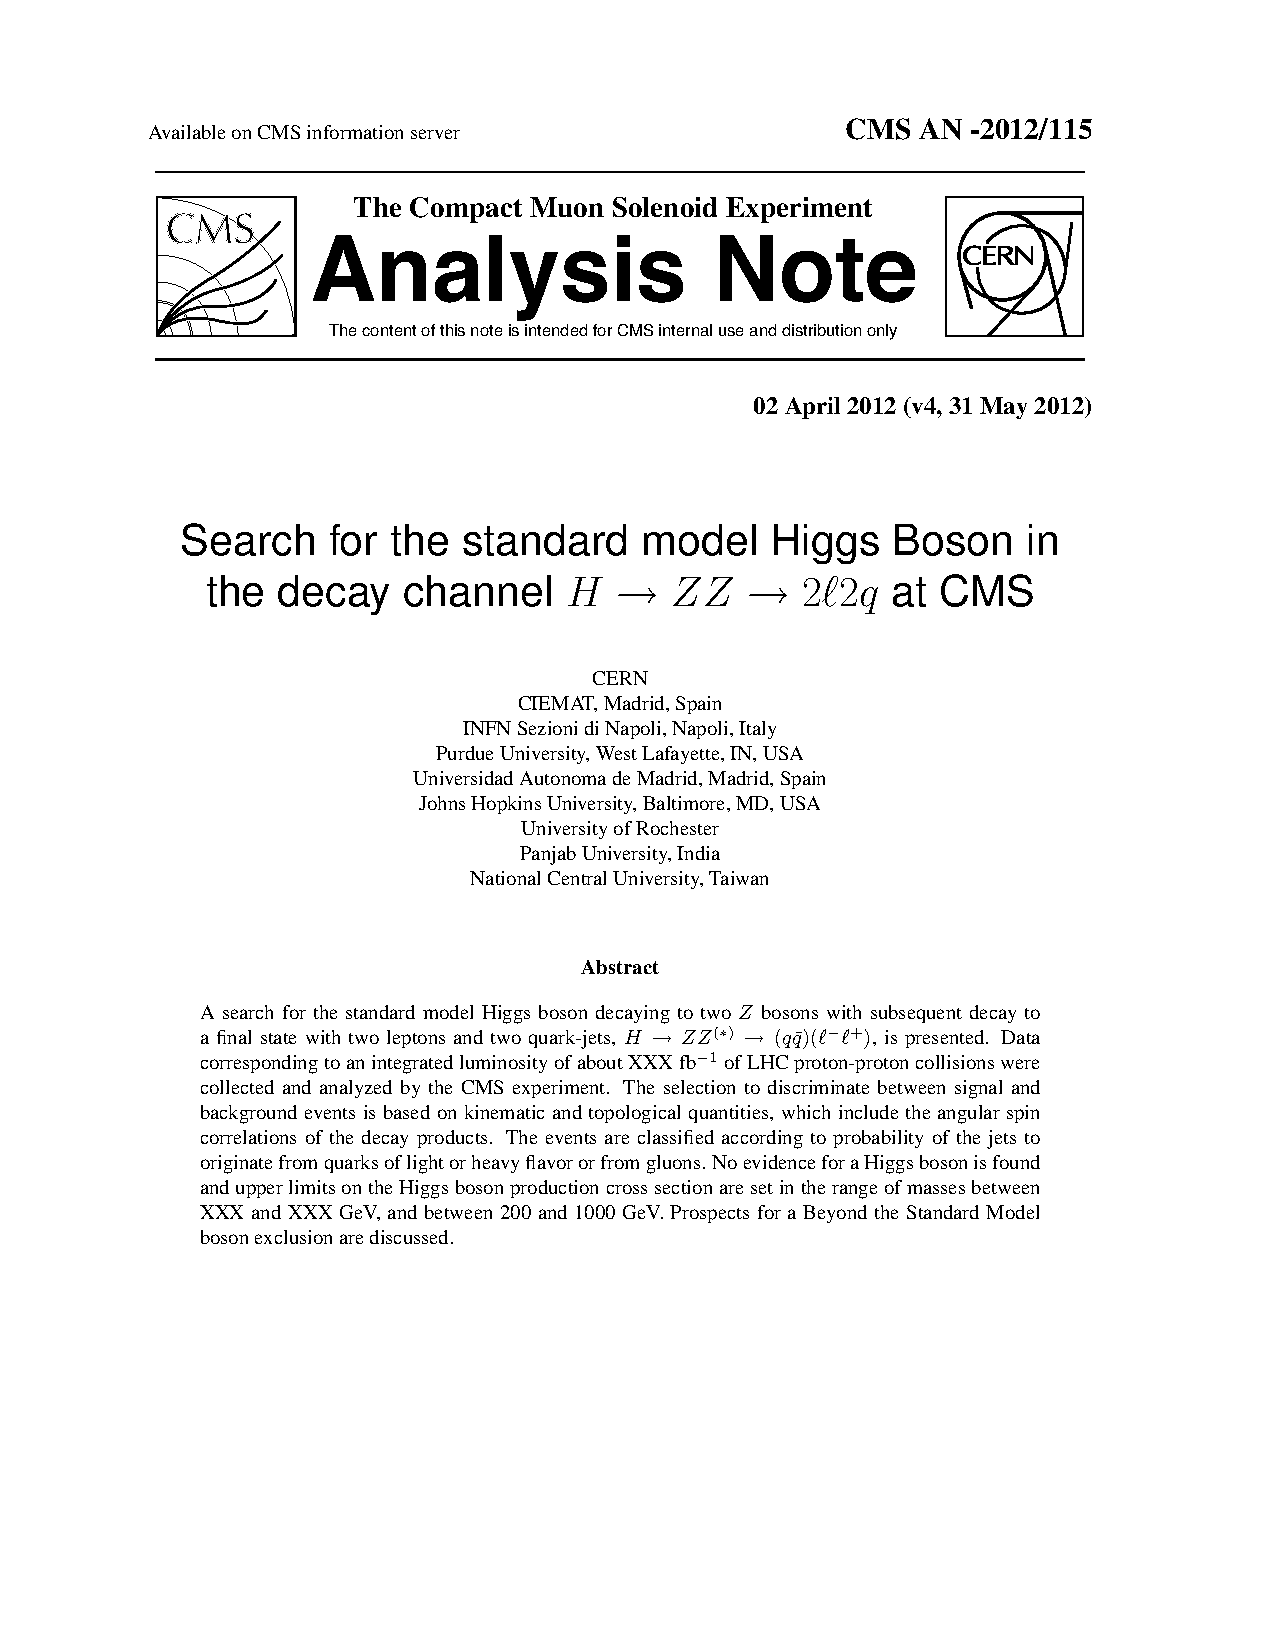
\includegraphics[width=0.5\textwidth]{images/AN2012_115.pdf}

%    \end{center}
%\end{frame}


%\section[Standard Model]{Standard Model}




%\section[Standard Model]{Standard Model}

\begin{frame}{Sub-atomic World}
\begin{center}
Particle Physics is the study of the properties of the fundamental building blocks of the universe and the interactions between them.
\\
\vspace{1em}
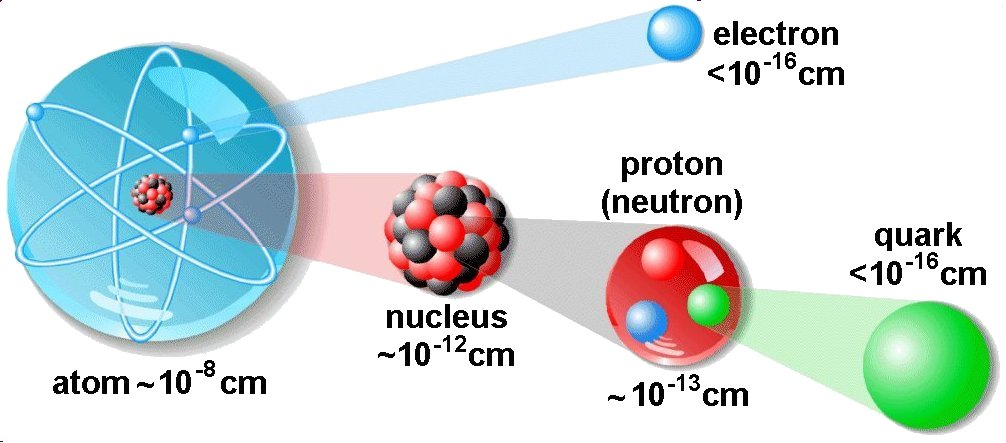
\includegraphics[width=0.99\textwidth]{images/subatomic_world.jpg}
\end{center}
\end{frame}


%\begin{frame}{Force}
%\begin{center}
%Force can be explained as the exchange of force carriers between particles.
%\\
%\vspace{1em}
%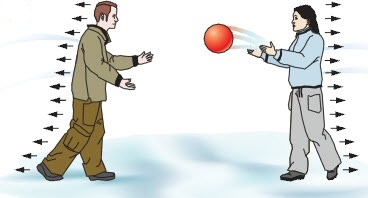
\includegraphics[width=0.69\textwidth]{images/force_exchange.jpg}
%\end{center}
%\end{frame}



\begin{frame}{The Four Fundamental Forces}
\begin{center}
There are four fundamental forces that we know of.
\\
\vspace{1em}
%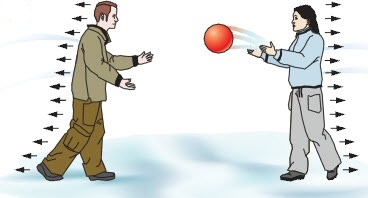
\includegraphics[width=0.69\textwidth]{images/force_exchange.jpg}
\begin{tabular}{ c c c c }
Force  & Boson    & Charge & Mass \\ \hline
Gravitational & graviton(G) & 0 & ? \\
Electromagnetic & photon($\gamma$) & 0 & 0 \\

\multirow{2}{*}{Weak} & W boson($W^{\pm}$) & $\pm$1 & 81 GeV \\
                      & Z boson(Z) & 0 & 92GeV \\

Strong & gluon(g) & 0      & 0 \\
\end{tabular}
\end{center}
\end{frame}




\begin{frame}{The Standard Model}
\begin{center}
The Standard Model is the compilation of over 100 years of scientific discoveries and is in excellent agreements with a wide range of experimental observations.
\\
\vspace{1em}
%\begin{columns}
 % \begin{column}{0.5\textwidth}
    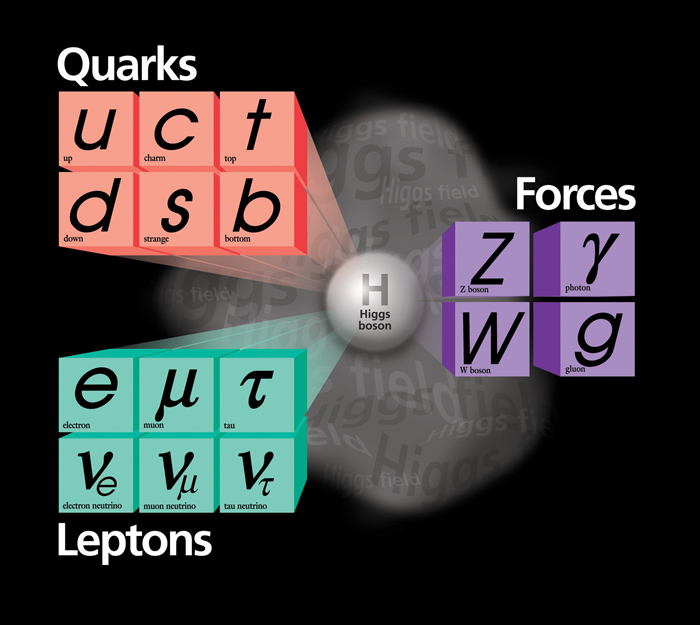
\includegraphics[width=0.49\textwidth]{images/standard_model_particles.jpg}
  %\end{column}
  %\begin{column}{0.5\textwidth}
  %\end{column}
\end{center}
\end{frame}

\begin{frame}{Particle Discoveries}
  \begin{center}
    \footnotesize
\begin{tabular}{ | c | c |}
  \hline
  Year & Discovery \\ \hline \hline
  1897 & e discovery, by J.J. Thompson (cathode ray tube, UK)\\ \hline
  1919 & proton, Ernest Rutherford (UK)\\ \hline
  1930 & neutron, James Chadwick (UK)\\ \hline
  1936 & m, Carl D. Anderson at Caltech\\ \hline
  1947 & strange quark(K+=usbar, K-=subar)\\ \hline
  1956 & $\nu_e$ discovery (nuclear reactor)\\ \hline
  1962 & $\nu_{\mu}$ discovery at BNL\\ \hline
  1968 & u and d quark (quark model)\\ \hline
  1974 & c quark (BNL, SLAC,J/y=ccbar)\\ \hline
  1977 & tau discovery (SLAC)\\ \hline
  1977 & b quark (Upsilon, FNAL)\\ \hline
  1979 & gluon (DESY)\\ \hline
  1983 & W and Z (CERN) \\ \hline
  1995 & top quark \\ \hline
  2000 & $\nu_t$ discovery (Fermilab) \\ \hline \hline
  2012 & ??Higgs?? (CERN) \\ \hline
\end{tabular}
\end{center}
\end{frame}


\begin{frame}{The Higgs Mechanism}
\scriptsize
\begin{itemize}
\item
  The potential on the left if symmetric as is the potential on the right.
\item
  The ground state symmetry is spontaneously broken in the potential on the right.
\end{itemize}
\begin{center}
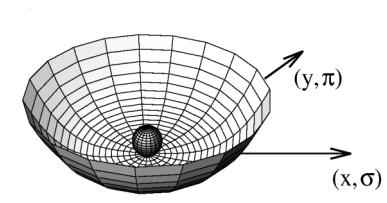
\includegraphics[width=0.49\textwidth]{images/higgs_mechanism.png}
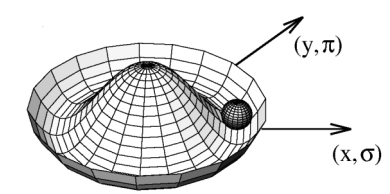
\includegraphics[width=0.49\textwidth]{images/higgs_mechanism_broken.png}
\end{center}
\begin{itemize}
\item
The Higgs field is the simplest of several proposed causes for electroweak symmetry breaking and the means by which elementary particles acquire mass.
\item
The Higgs boson is the smallest possible excitation of the Higgs field.
\end{itemize}
%\begin{itemize}
%\item
%  When you have spontaneous symmetry breaking you get Goldstone bosons.
%\item
%  Peter Higgs showed that when a local symmetry is spontaneously broken in a relativistic theory instead of Goldstone bosons you get a m%assive vector field.
%\item
%  The other mode is a massive spin-zero particle (Higgs boson).
%\end{itemize}
\end{frame}


%\begin{frame}{Higgs ``Description'' }
%\begin{center}
%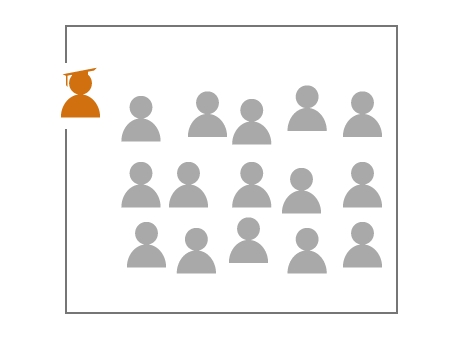
\includegraphics[width=0.89\textwidth]{images/higgs_cartoon-0.png}
%\end{center}
%\end{frame}

%\begin{frame}{Higgs ``Description'' }
%\begin{center}
%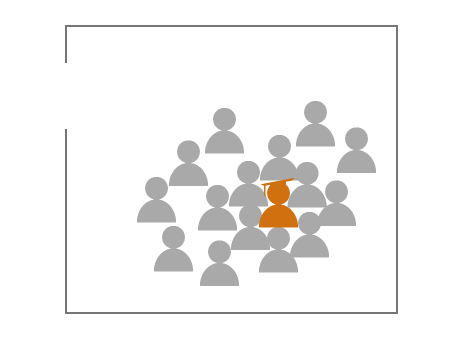
\includegraphics[width=0.89\textwidth]{images/higgs_cartoon-1.png}
%\end{center}
%\end{frame}

%\begin{frame}{Higgs ``Description'' }
%\begin{center}
%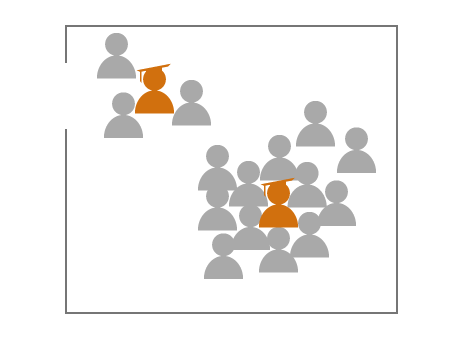
\includegraphics[width=0.89\textwidth]{images/higgs_cartoon-2.png}
%\end{center}
%\end{frame}



\section{LHC Search for Higgs Boson}


\begin{frame}{The Standard Model}
\begin{center}
The Standard Model is the compilation of over 100 years of scientific discoveries and is in excellent agreement with a wide range of experimental observations.
\\
\vspace{1em}
\begin{columns}
  \begin{column}{0.5\textwidth}
    \begin{center}
    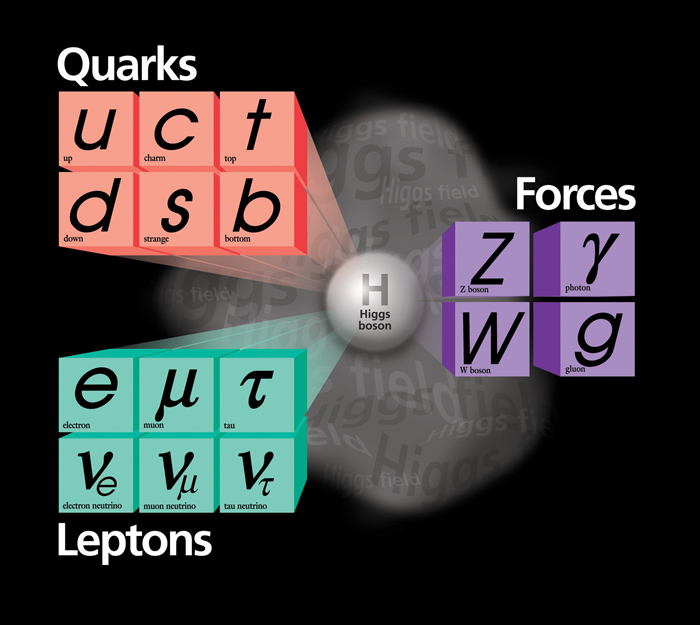
\includegraphics[width=.95\textwidth]{images/standard_model_particles.jpg}\vspace{.1em}
    %\tiny{Source: \url{http://www.fnal.gov/pub/presspass/press_releases/2013/Higgs-Boson-20130314.html}}
    {\fontsize{.1cm}{.001em}\selectfont Source: \url{http://www.fnal.gov/pub/presspass/press_releases/2013/Higgs-Boson-20130314.html}}
    \end{center}
  \end{column}
  \begin{column}{0.5\textwidth}
\begin{center}
\begin{itemize}
  \item
In the Standard Model the simplest solution for the nature of the electroweak symmetry breaking is the introduction of the Higgs field.
\item 
%\vspace{1em}
At the comencement of the LHC the only free parameter of the Standard Model was the Higgs mass.
\end{itemize}
\end{center}
  \end{column}
\end{columns}
\end{center}
\end{frame}

\begin{frame}{Experimental Constraints on the SM Higgs Mass}
\begin{center}
\begin{columns}
      \begin{column}{0.5\textwidth}
        \begin{center}
%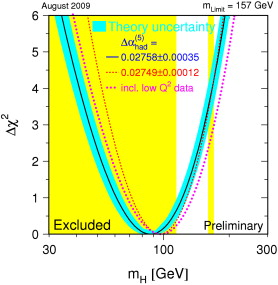
\includegraphics[width=0.99\textwidth]{images/LEPtevatron2009.jpg}
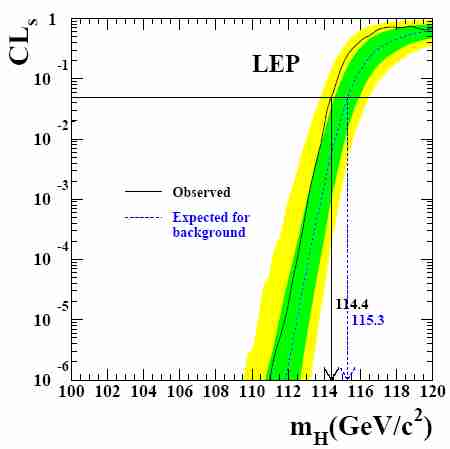
\includegraphics[width=0.65\textwidth]{images/lep2limit.jpg}\\
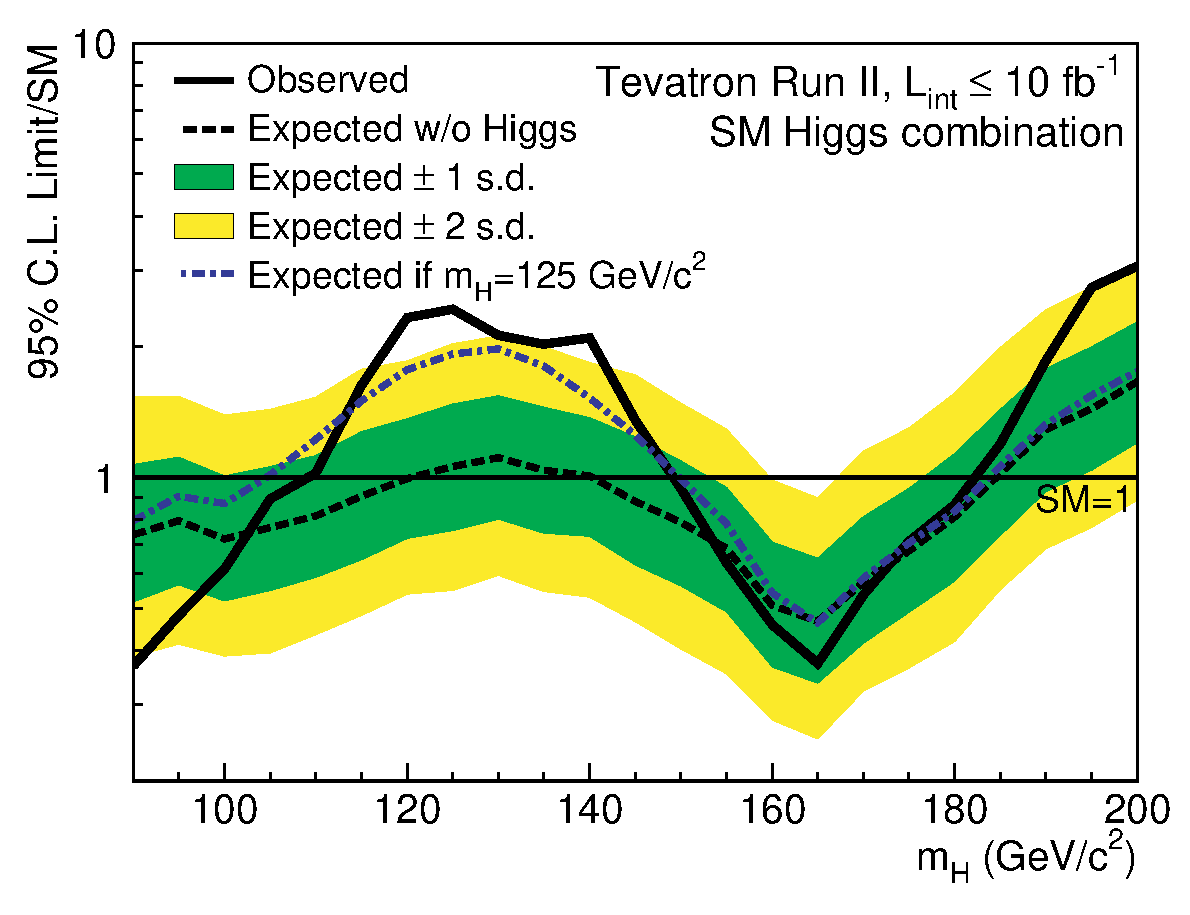
\includegraphics[width=0.75\textwidth]{images/tevsmlimits_feb2013.eps}\\
%\vspace{.001em}
{\fontsize{.1cm}{.001em}\selectfont Source: \url{http://tevnphwg.fnal.gov/}}
\end{center}
\end{column}
\begin{column}{0.5\textwidth}
Experimental constraints:
\begin{itemize}
\item
  LEP excluded with $CL_{95\%}$\\
  \vspace{.5em}
  $m_H$ < 114.4 GeV.\\
  \vspace{1em}
\item
  The latest measurments from Tevetron (July 2013) exclude with $CL_{95\%}$ at:\\
  \vspace{.5em}
  90 GeV < $m_H$ < 109 GeV\\
  149 GeV < $m_H$ < 182 GeV.
\end{itemize}
\end{column}
\end{columns}
\end{center}
\end{frame}

\begin{frame}{Why search for a Higgs at high mass?}
\begin{block}{Discovery}
In 2012 ATLAS and CMS announced the discovery of a new boson at 126 GeV.  In 2013 is was confirmed that this new particle is consistant with a Standard Model Higgs boson.
\end{block}
This analysis is sensative in the 250 to 650 GeV range so why search there?
\begin{itemize}
\item
When we started this analysis in 2011 we didn't know where the Higgs boson would be. (Needed to look everywhere)
\item
Is the new particle THE Standard Model Higgs boson.
\item
Are there other Higgs bosons?
\end{itemize}
\footnotesize
\begin{block}{Beyond the Standard Model}
Many Beyond the Standard Model (BSM) theories extend the simple Higgs sector of the Standard Model and lead to more complicated particle spectrum. Very often one of the new particles has properties similar to the Standard Model Higgs.
\end{block}
\end{frame}





%\begin{frame}{The Higgs Mechanism}
%\begin{center}
%  \begin{itemize}
%  \item
%    A simple solution for the nature of the electroweak symmetry breaking is introducing the Higgs field.
%  \item
%    The Higgs field is also the means by which elementary particles acquire mass.
%  \item
%    The Higgs boson is the smallest possible excitation of the Higgs field.
%  \item
%    The Higgs mass is a free parameter.
%  \end{itemize}
%\end{center}
%\end{frame}


%\begin{frame}{Particle Accelerators}
%\begin{center}
%Particle accelerators accelerate particles to high energies.
%\begin{columns}
%  \begin{column}{0.4\textwidth}
%This allows us to:
%    \begin{itemize}
%    \item
%      Look deeper into matter (E $\propto \dfrac{1}{size}$ ). ``microscope''
%    \item
%      Discover new heavier particles ($E = mc^{2}$).
%    \item
%      Probe early conditions of the Universe (E = kT).
%    \end{itemize}
%  \end{column}
%  \begin{column}{0.6\textwidth}
%    \begin{center}
%    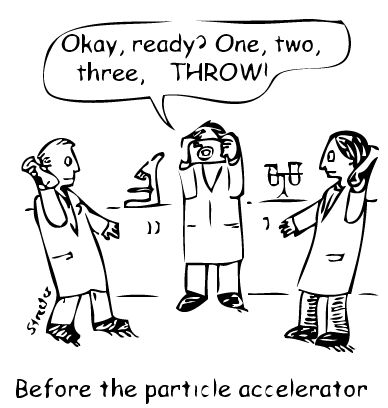
\includegraphics[width=0.79\textwidth]{images/before_accelerators.png}
%    \end{center}
%  \end{column}
%\end{columns}
%All this while being controlled in the laboratory.
%\end{center}
%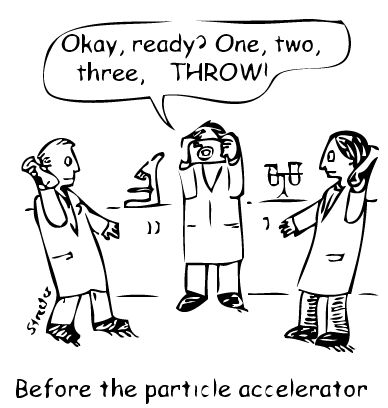
\includegraphics[width=0.99\textwidth]{images/before_accelerators.png}
%\end{frame}


%\begin{frame}{LHC}
%\begin{center}
%Four Experiments
%\begin{itemize}
%\item
%  CMS - General Purpose
%\item
%  ATLAS - General Purpose
%\item
%  LHCb - b-physics
%\item
%  ALICE - heavy ion
%\end{itemize}
%\vspace{.5em}
%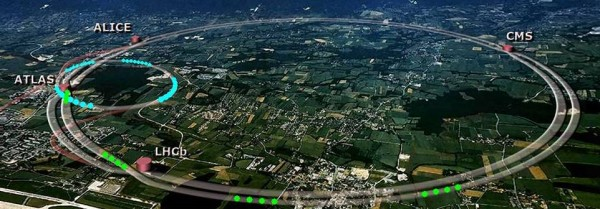
\includegraphics[width=0.99\textwidth]{images/lhc-sim-600x209.jpg}
%\end{center}
%\end{frame}



%\begin{frame}{The LHC Accelerator}
%  \begin{center}
%    \begin{itemize}
%    \item
%      Proton-proton collider
%    \item
%      Circumference: 26.7 km
%    \item
%      Tunnel: 100 meters underground
%    \item
%      dipoles operate at 8.3 T
%    \item
%      1232 superconducting Niobium-Titanium magnets
%    \item
%      better vacuum and colder than inter-planetary  space
%    \end{itemize}
  
%\vspace{.5em}
%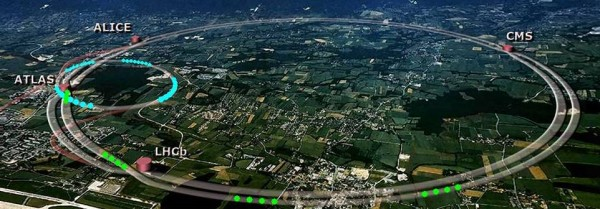
\includegraphics[width=0.99\textwidth]{images/lhc-sim-600x209.jpg}

%  \end{center}
%\end{frame}





%\begin{frame}{Injection Scheme}
%\begin{center}
%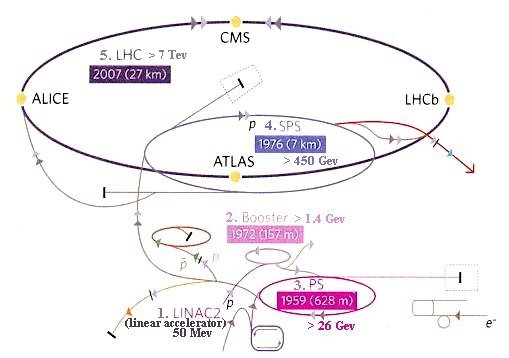
\includegraphics[width=0.49\textwidth]{images/lhc_schematic.jpg}
%\begin{itemize}
%\item
%Linac2 $\rightarrow$ 50 MeV
%\item
%Proton Synchrotron  $\rightarrow$ 1.4 GeV
%\item
%Super Protron Synchrotron  $\rightarrow$ 450 GeV
%\item
%LHC  $\rightarrow$ 4.0 TeV
%\end{itemize}
%\end{center}
%\end{frame}


\begin{frame}{LHC Environment}
%\begin{center}
\begin{columns}
\begin{column}{0.5\textwidth}
\begin{center}
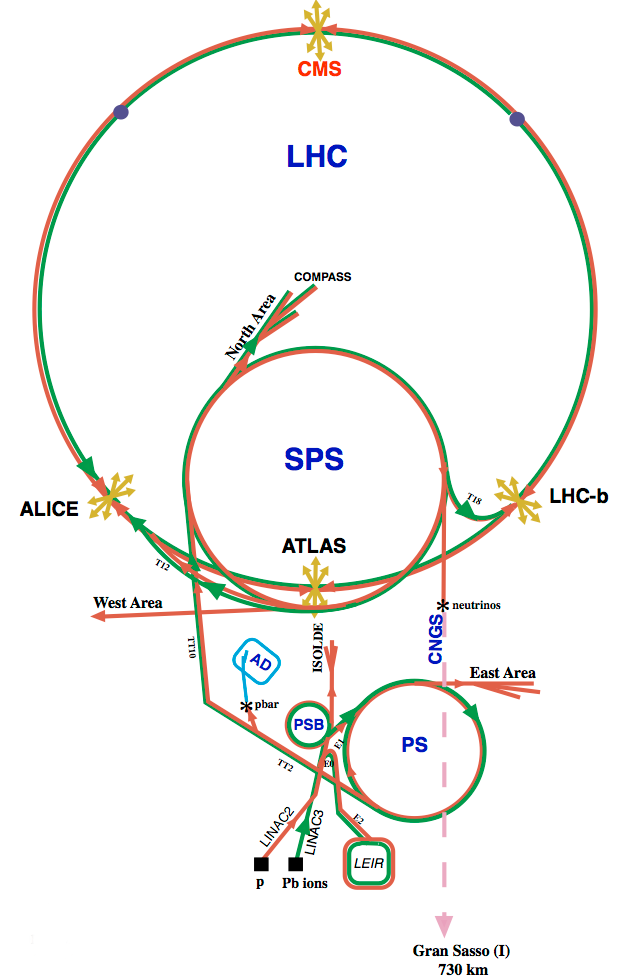
\includegraphics[width=0.79\textwidth]{images/cern-acc.png}\\
{\fontsize{.1cm}{.001em}\selectfont Source: \url{http://www.quantumdiaries.org/2011/10/24/the-25-ns-pumpkin-teeth/}}
\end{center}
\end{column}
\begin{column}{0.5\textwidth}
\begin{center}
In 2012 $\sqrt{s}$ = 8 TeV\\
\vspace{.8em}
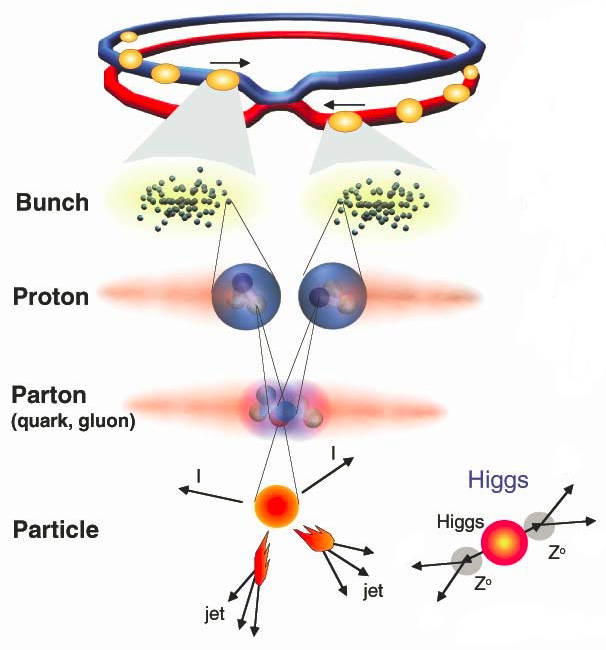
\includegraphics[width=0.89\textwidth]{images/HKrT0L.png}\\
{\fontsize{.1cm}{.001em}\selectfont Source: \url{Haijun Yang, Colloquium Shanghai Jian Tong University, Sept 12, 2012}}
\end{center}
\end{column}
\end{columns}
%
%HKrT0L.png
%\end{center}
\end{frame}


\begin{frame}{LHC Delivered Data}

\begin{columns}
\begin{column}{0.5\textwidth}
\begin{center}
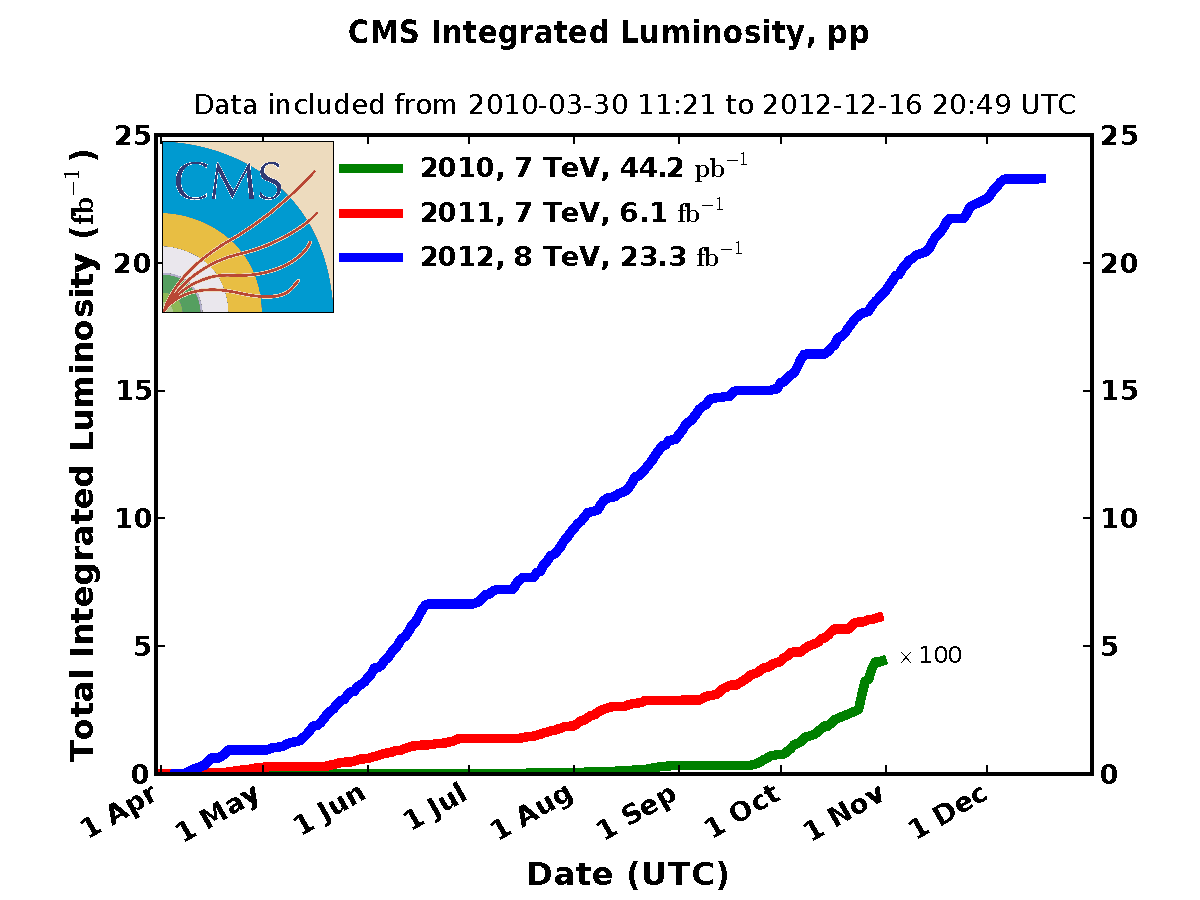
\includegraphics[width=0.85\textwidth]{images/int_lumi_cumulative_pp_2.pdf}\\
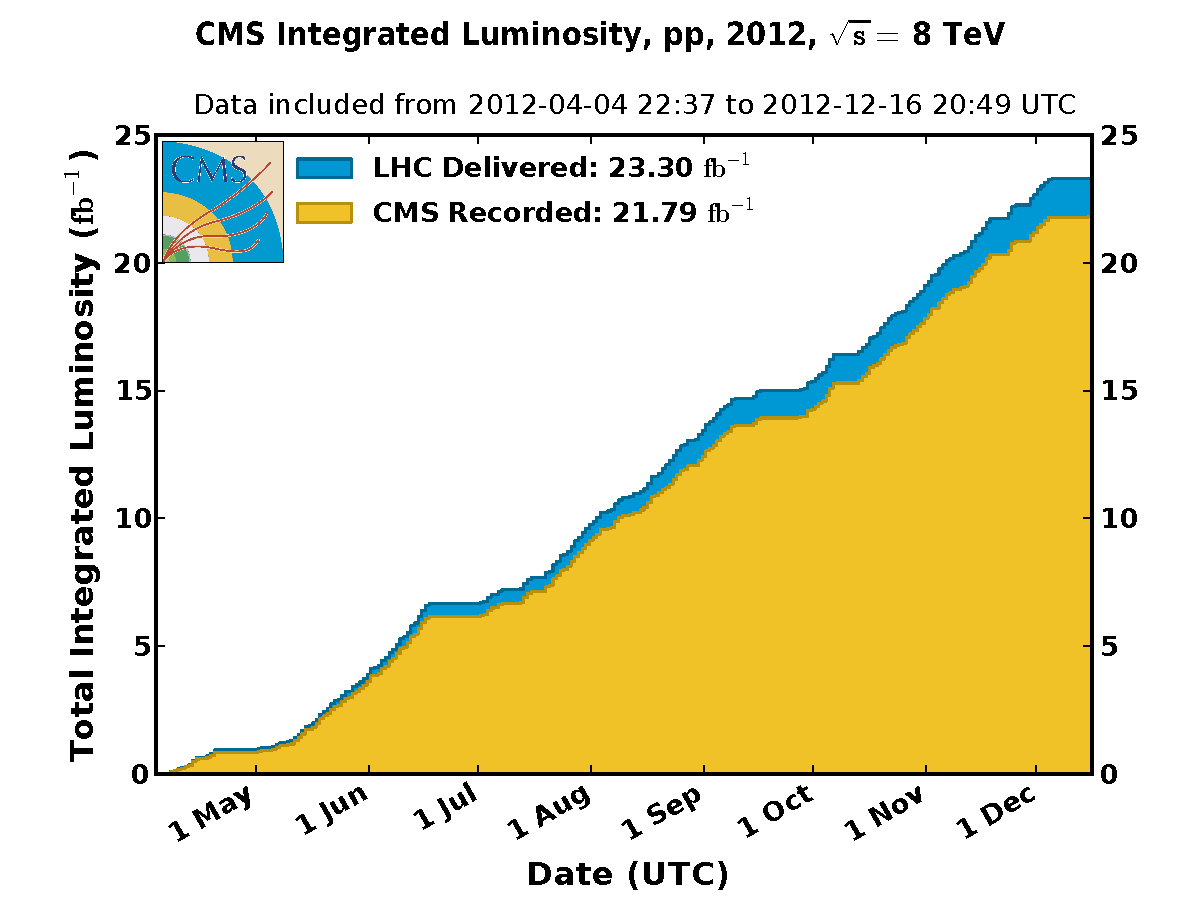
\includegraphics[width=0.85\textwidth]{images/int_lumi_per_day_cumulative_pp_2012.pdf}\\
\end{center}
\end{column}
\begin{column}{0.5\textwidth}
\begin{itemize}
\item
CMS has done extremely well during Run I (2010-2012).
\item
Data-taking efficiency was very high (95\%)
\item
Main challenge of the 2012 was how to deal with pileup.
\end{itemize}
\begin{center}
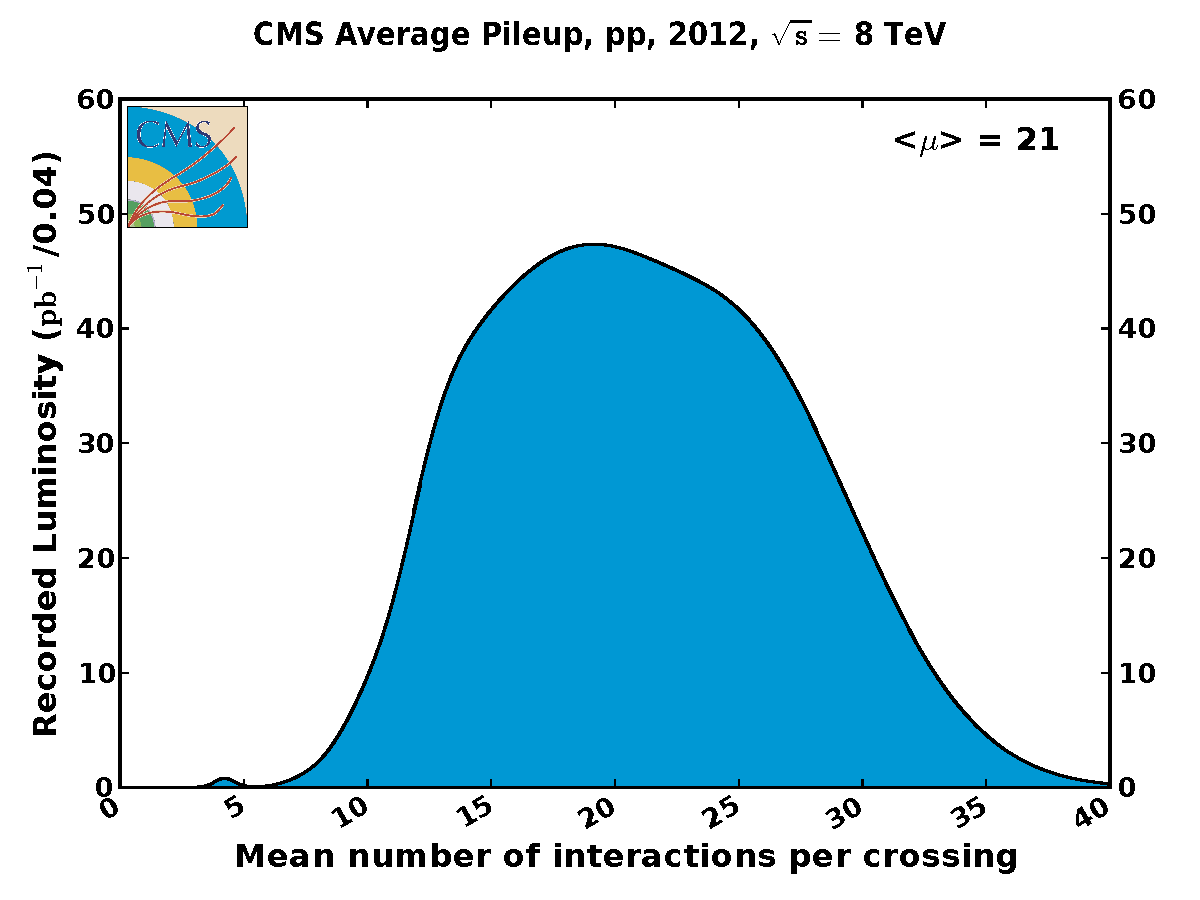
\includegraphics[width=0.85\textwidth]{images/pileup_pp_2012.pdf}
{\fontsize{.1cm}{.001em}\selectfont Source: \url{http://twiki.cern.ch/twiki/bin/view/CMSPublic/LumiPublicResults}}
\end{center}
\end{column}
\end{columns}

%\begin{center}
%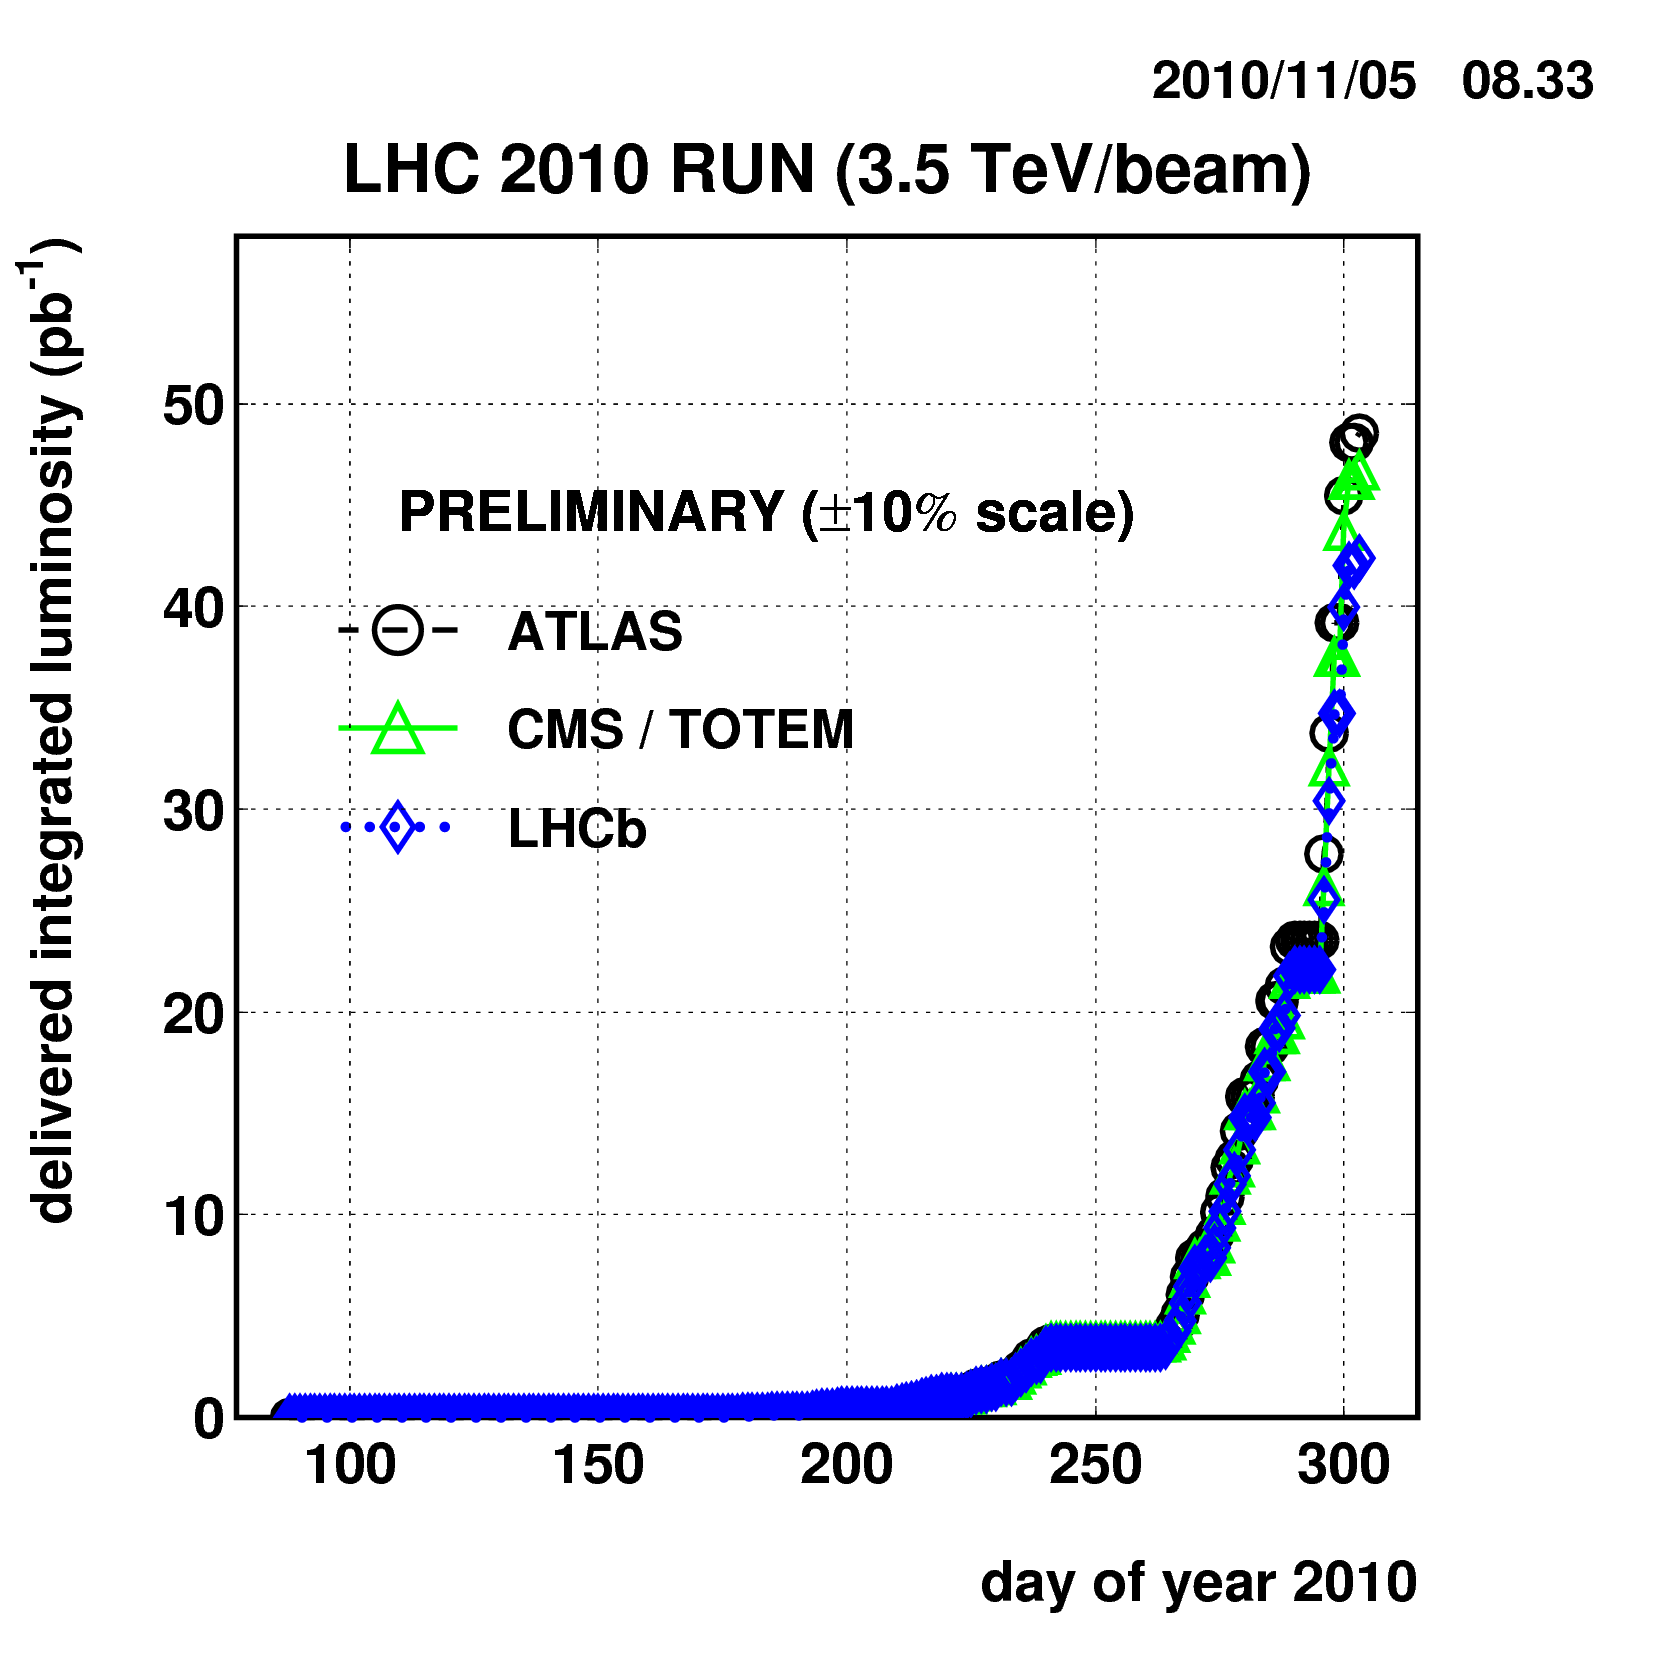
\includegraphics[width=0.33\textwidth]{images/2010_lhc_luminocity.png}
%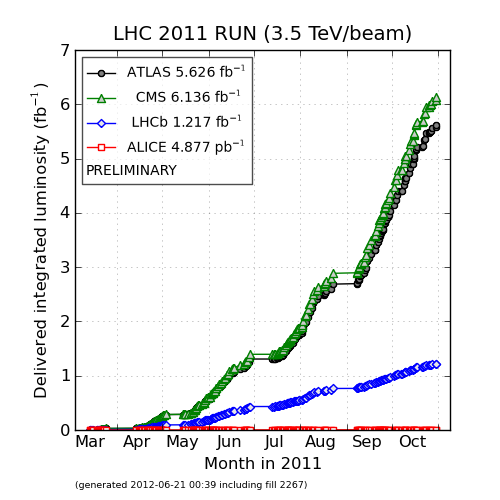
\includegraphics[width=0.33\textwidth]{images/2011_lhc_luminocity.png}
%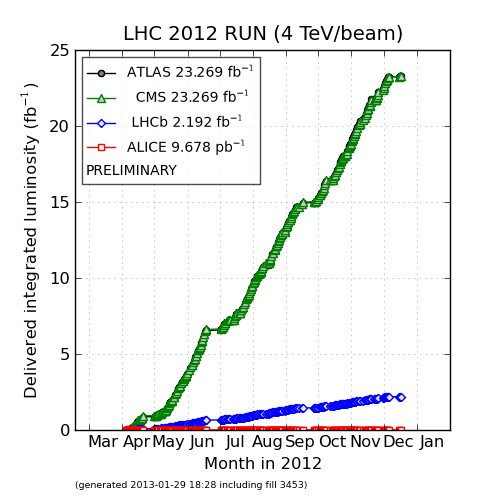
\includegraphics[width=0.33\textwidth]{images/2012_lhc_luminocity.png}
%\end{center}
\end{frame}

\begin{frame}{Compact Muon Solenoid}
\begin{center}
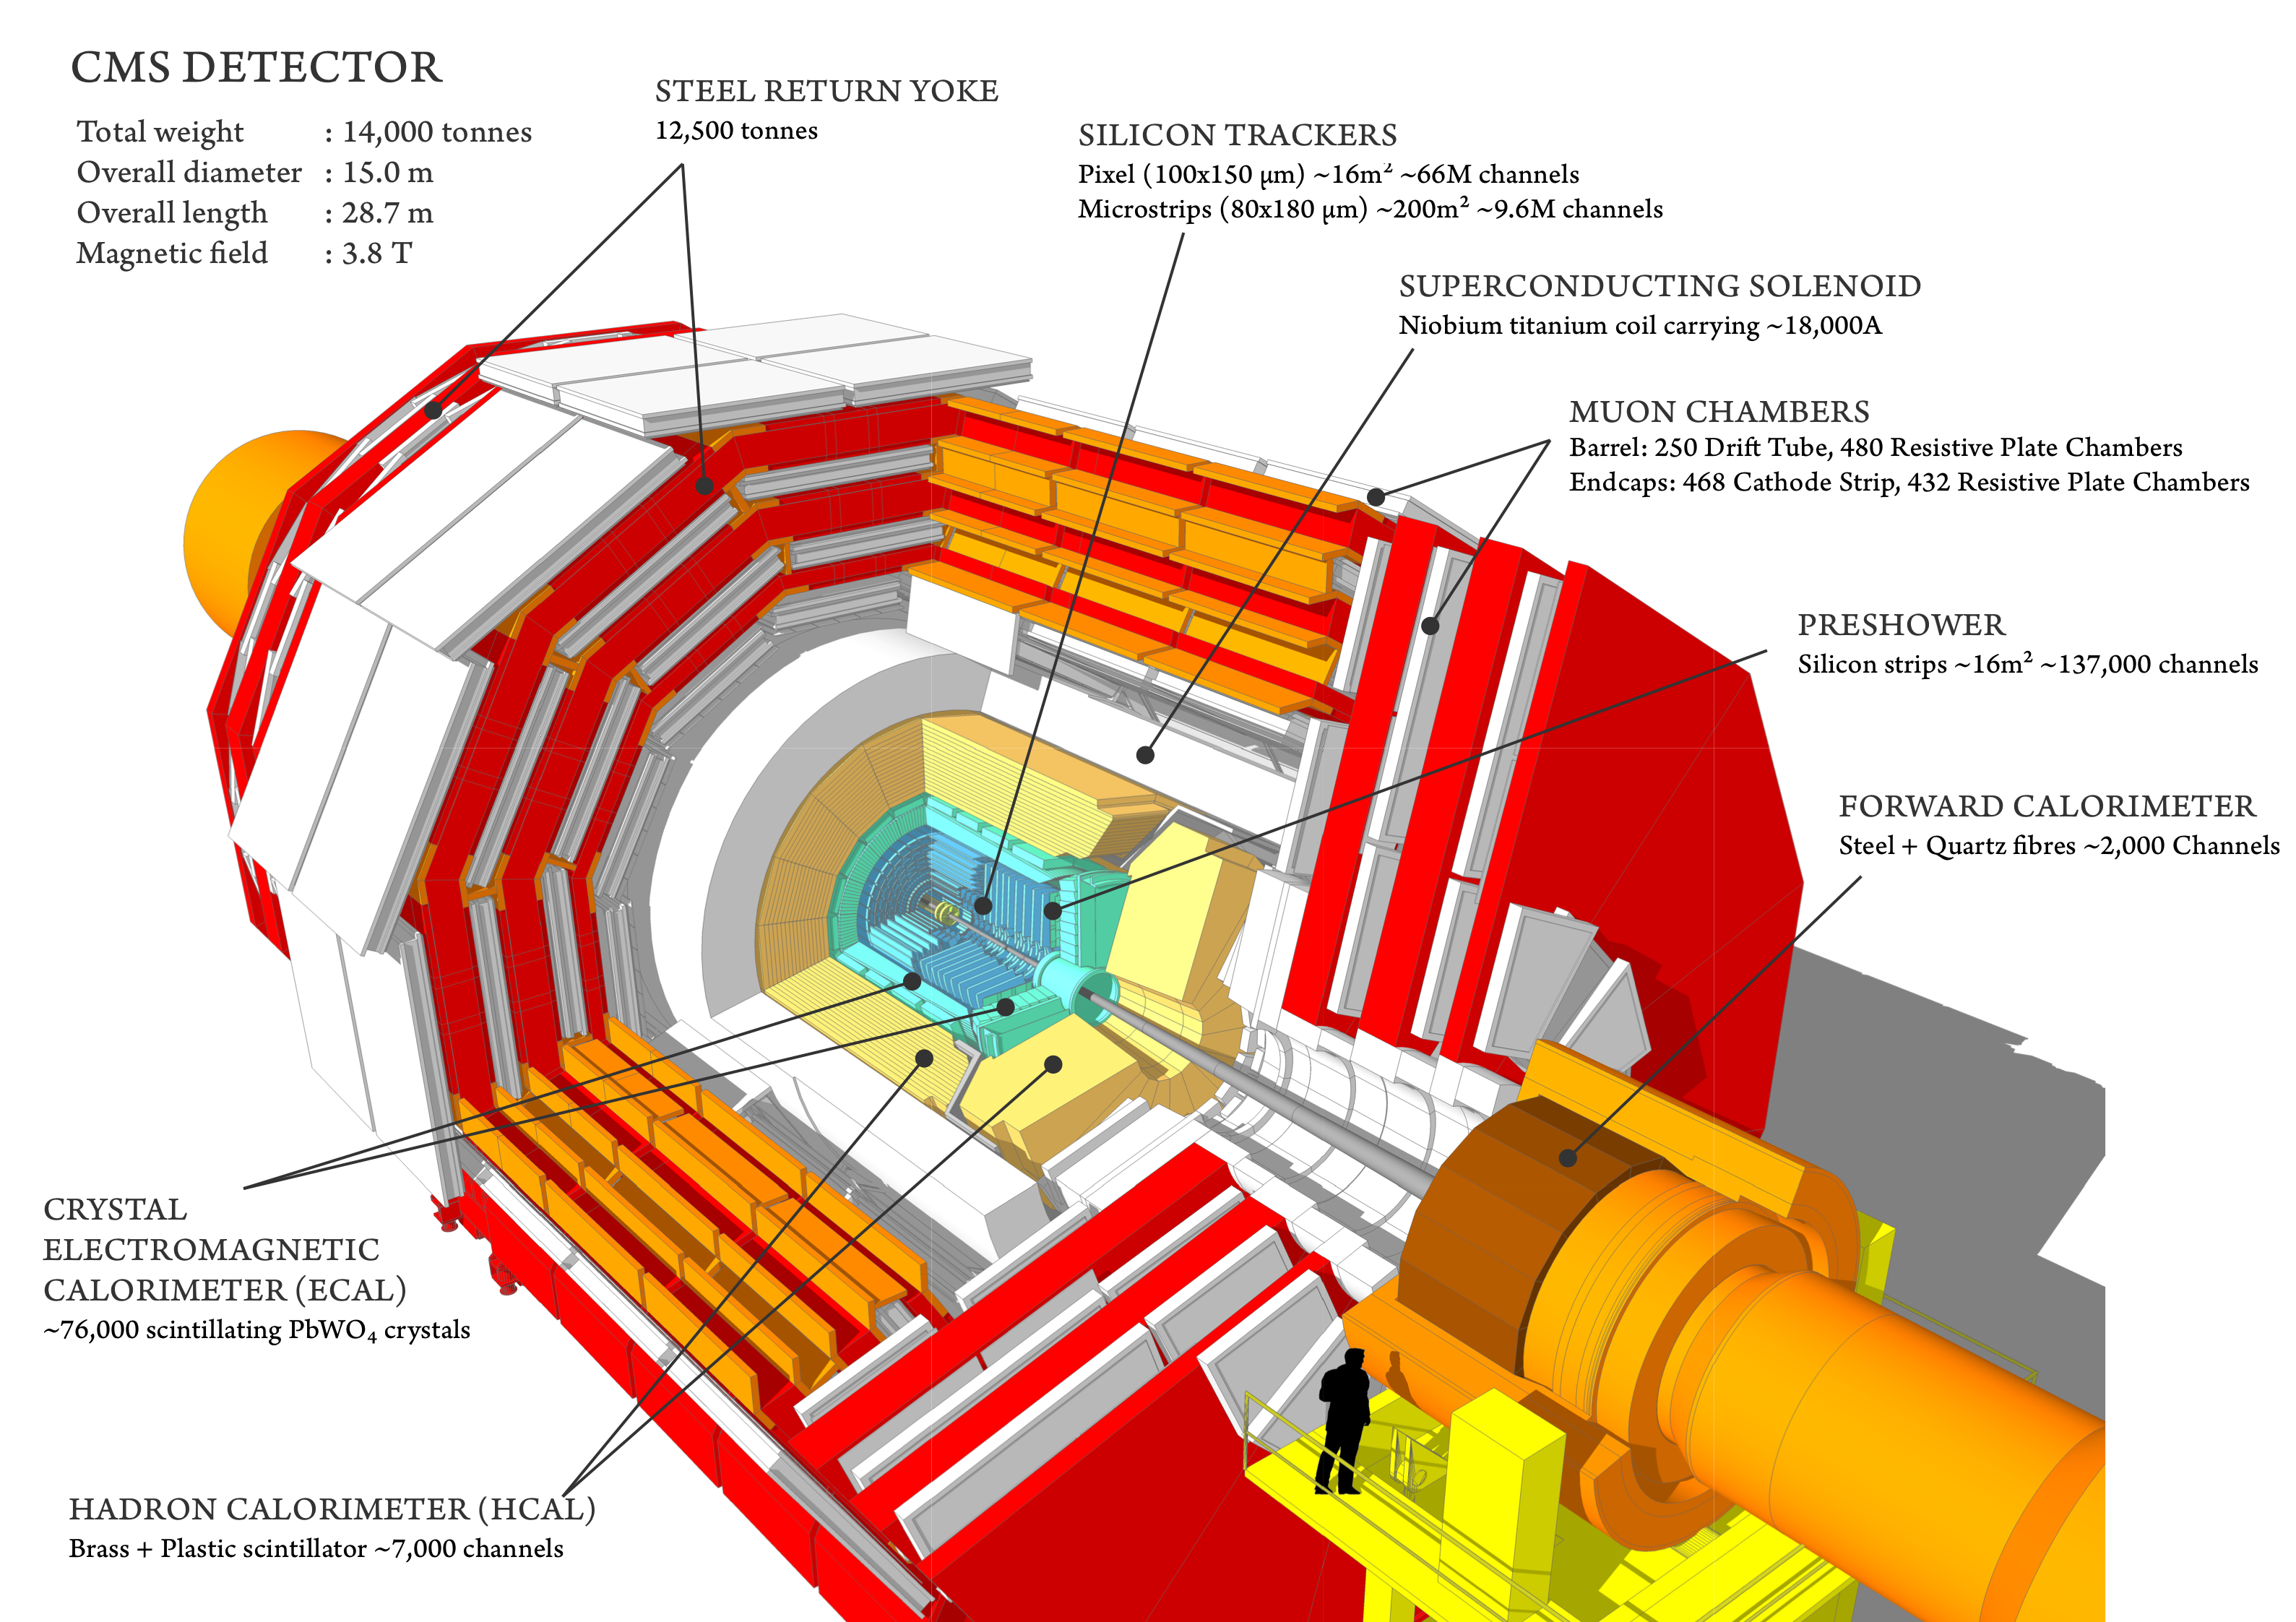
\includegraphics[width=0.85\textwidth]{images/cms_120918_03.png}\\
{\fontsize{.1cm}{.001em}\selectfont Source: \url{http://www.fnal.gov/pub/presspass/press_releases/2013/Higgs-Boson-20130314.html}}
%/CMScollaborationPoster.png}

\end{center}
\end{frame}


\begin{frame}{CMS Slice}
\begin{center}
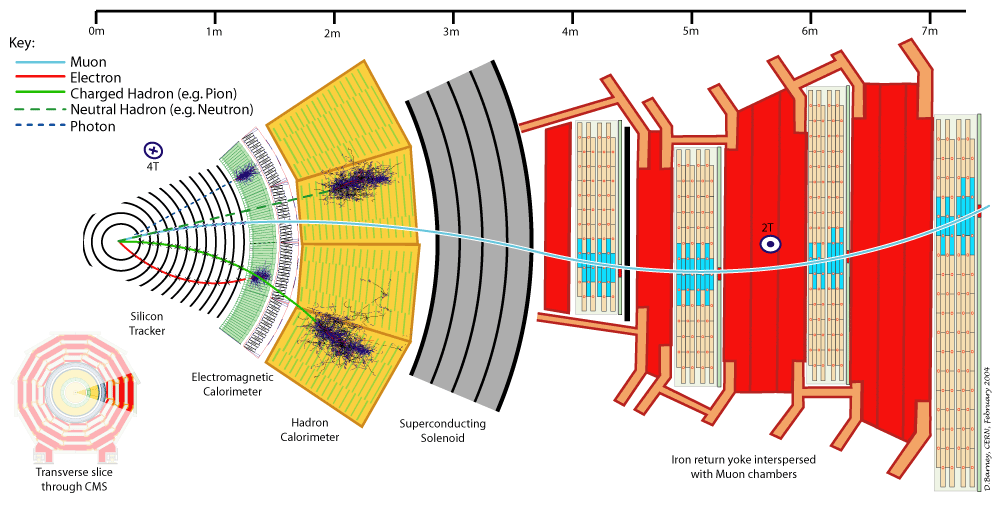
\includegraphics[width=0.99\textwidth]{images/CMS_Slice.png}
\end{center}
\end{frame}

\begin{frame}{CMS Detector Glossary}
\begin{center}
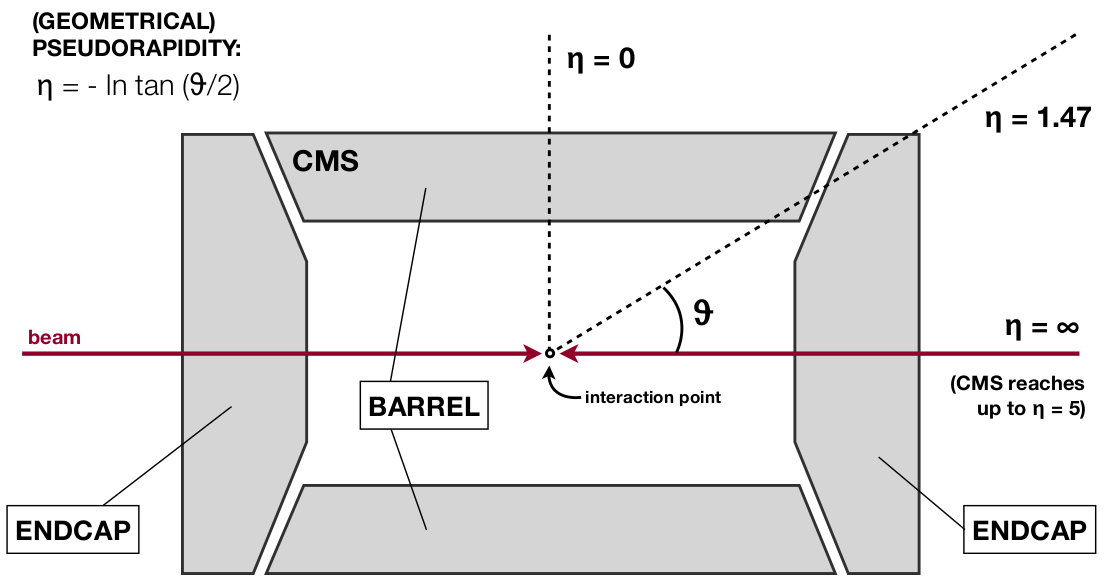
\includegraphics[width=0.99\textwidth]{images/DetectorGlossary.png}
\end{center}
\end{frame}

%\begin{frame}{Space Holder}
%\begin{center}
%\end{center}
%\end{frame}

\begin{frame}{Higgs Production}
\begin{center}
\begin{columns}
  \begin{column}{0.35\textwidth}
    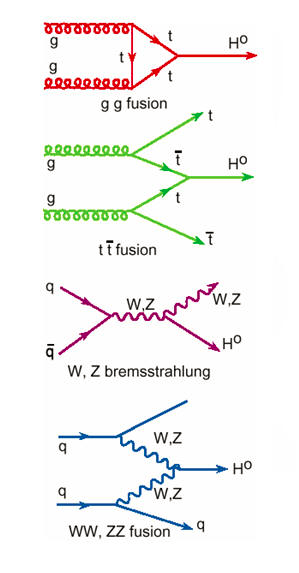
\includegraphics[width=0.99\textwidth]{images/higgs_production_feynman.png}
  \end{column}
  \begin{column}{0.65\textwidth}
    Gluon-gluon fusion ($gg \rightarrow H$) and vector-boson fusion ($qq \rightarrow qqH$) are dominant
    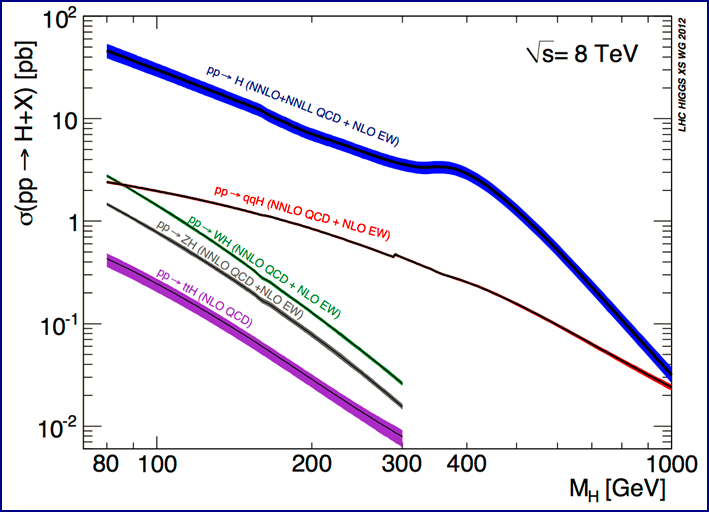
\includegraphics[width=0.99\textwidth]{images/higgs_production_lhc.png}
  \end{column}
\end{columns}
\end{center}
\end{frame}








\begin{frame}{Higgs Decay}
\begin{center}
\begin{columns}
  \begin{column}{0.5\textwidth}
    \begin{itemize}
      \item
        Discovery strategy depends on the available decay channels.
      \item
        Decays with leptons provide clean signatures.
    \end{itemize}
  \end{column}
  \begin{column}{0.5\textwidth}
    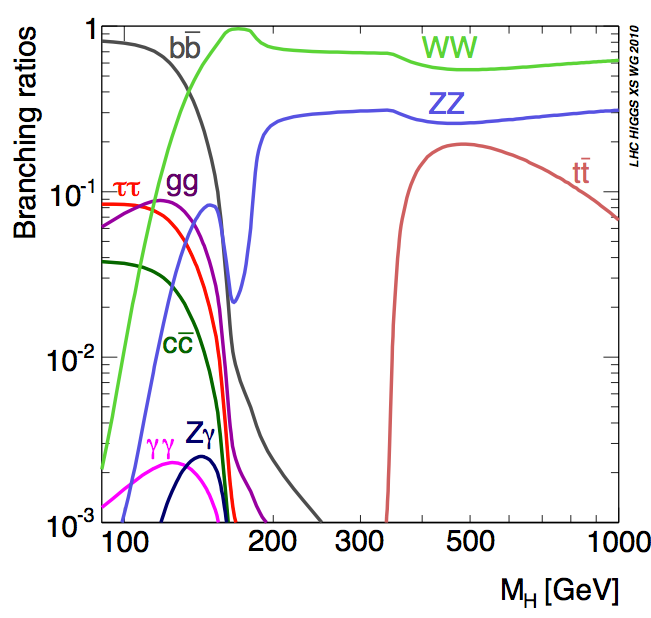
\includegraphics[width=0.99\textwidth]{images/branching_ratio.png}
  \end{column}
\end{columns}
Main Discovery Channels
\begin{itemize}
\item
  $H \rightarrow \gamma \gamma$
\item
  $H \rightarrow W^+W^-$
\item
  $H \rightarrow ZZ$
\end{itemize}
\end{center}
\end{frame}


\begin{frame}{The $H \rightarrow ZZ \rightarrow llqq$ Channel}
\begin{center}
There are three sub-channels in $H \rightarrow ZZ$ that are studied.\\
$H \rightarrow ZZ \rightarrow 4l$\\
$H \rightarrow ZZ \rightarrow 2l2 \nu$\\
\textcolor{red}{$H \rightarrow ZZ \rightarrow \Plp \Plm \Pq \Paq$\\
\scriptsize{$(\Pl =e, \mu$ and $q = u,d,c,s,b)$}}\\
\vspace{.5em}
\small
\begin{columns}
  \begin{column}{0.7\textwidth}
     Pros:\footnotesize
     \begin{itemize}
     \item
     Large branching ratios
     \begin{itemize}
     \item
       BR($Z \rightarrow qq$) = 70\%
     \item
       BR($ZZ \rightarrow 2l2q$) = $\color{red}{20} \color{black} \times BR(ZZ \rightarrow 4l)$
     \end{itemize}
   \item
     Full decay is reconstructed (closed kinematics)
     \end{itemize}
     \vspace{1em}
     \small
     Cons:\footnotesize
     \begin{itemize}
     \item
       Quarks hadronize to form ``jets.''
     \item
       Momentum resolution is worse for jets then for leptons.
     \item
       Large background coming from Z production in conjunction with QCD jets ($\sim 10^5$ > signal).
     \end{itemize}
  \end{column}
  \begin{column}{0.3\textwidth}
    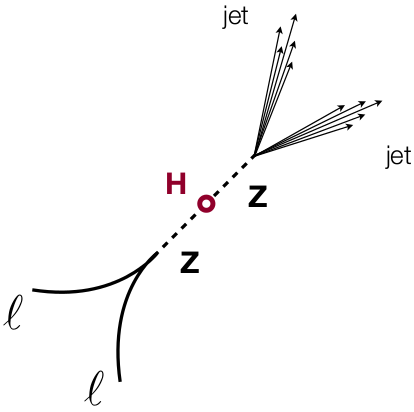
\includegraphics[width=0.99\textwidth]{images/h_zz_2l2q.png}
  \end{column}
\end{columns}
\end{center}
\end{frame}



%\begin{frame}{Traditional Jet Approach: Caloremeter Jets}
%\end{frame}



%\begin{frame}{Traditional Jet Approach: Calorimeter Jets}
%For CaloJets we assume most particles will reach the calorimeters close to each other.  So all we have to do is cluster the energy deposits in the calorimeters.

%\begin{columns}[T]
%  \begin{column}{0.6\textwidth}
%    \vspace{2em}
%    \begin{column}{0.5\textwidth}
%      Pros:
%      \begin{itemize}
%      \item
%        straightforward
%      \item
%        fast and unaffected by event complexity
%      \end{itemize}
%    \end{column}
%    \begin{column}{0.5\textwidth}
%      Cons:
%      \begin{itemize}
%      \item
%        response is $p_{T}$-dependent
%      \item
%        lose low $p_{T}$ charged particles
%      \item
%        limited by HCAL resolution
%      \end{itemize}
%    \end{column}
%  \end{column}
%  \begin{column}{0.40\textwidth}
%    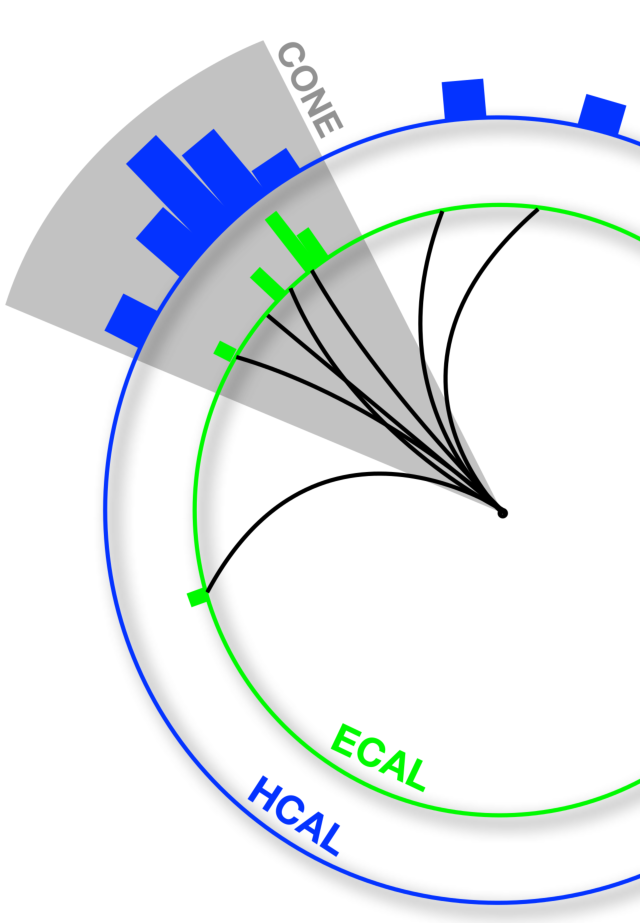
\includegraphics[width=0.99\textwidth]{images/calojets.pdf}
%  \end{column}
%\end{columns}
%\end{frame}



%\begin{frame}{Discovering the Higgs}
%\begin{center}
%\begin{columns}
%  \begin{column}{0.5\textwidth}
%  \end{column}
%  \begin{column}{0.5\textwidth}
%  \end{column}
%\end{columns}
%\end{center}
%\end{frame}


\section{Event Selection}


\begin{frame}{Analysis workflow}
  \begin{center}
  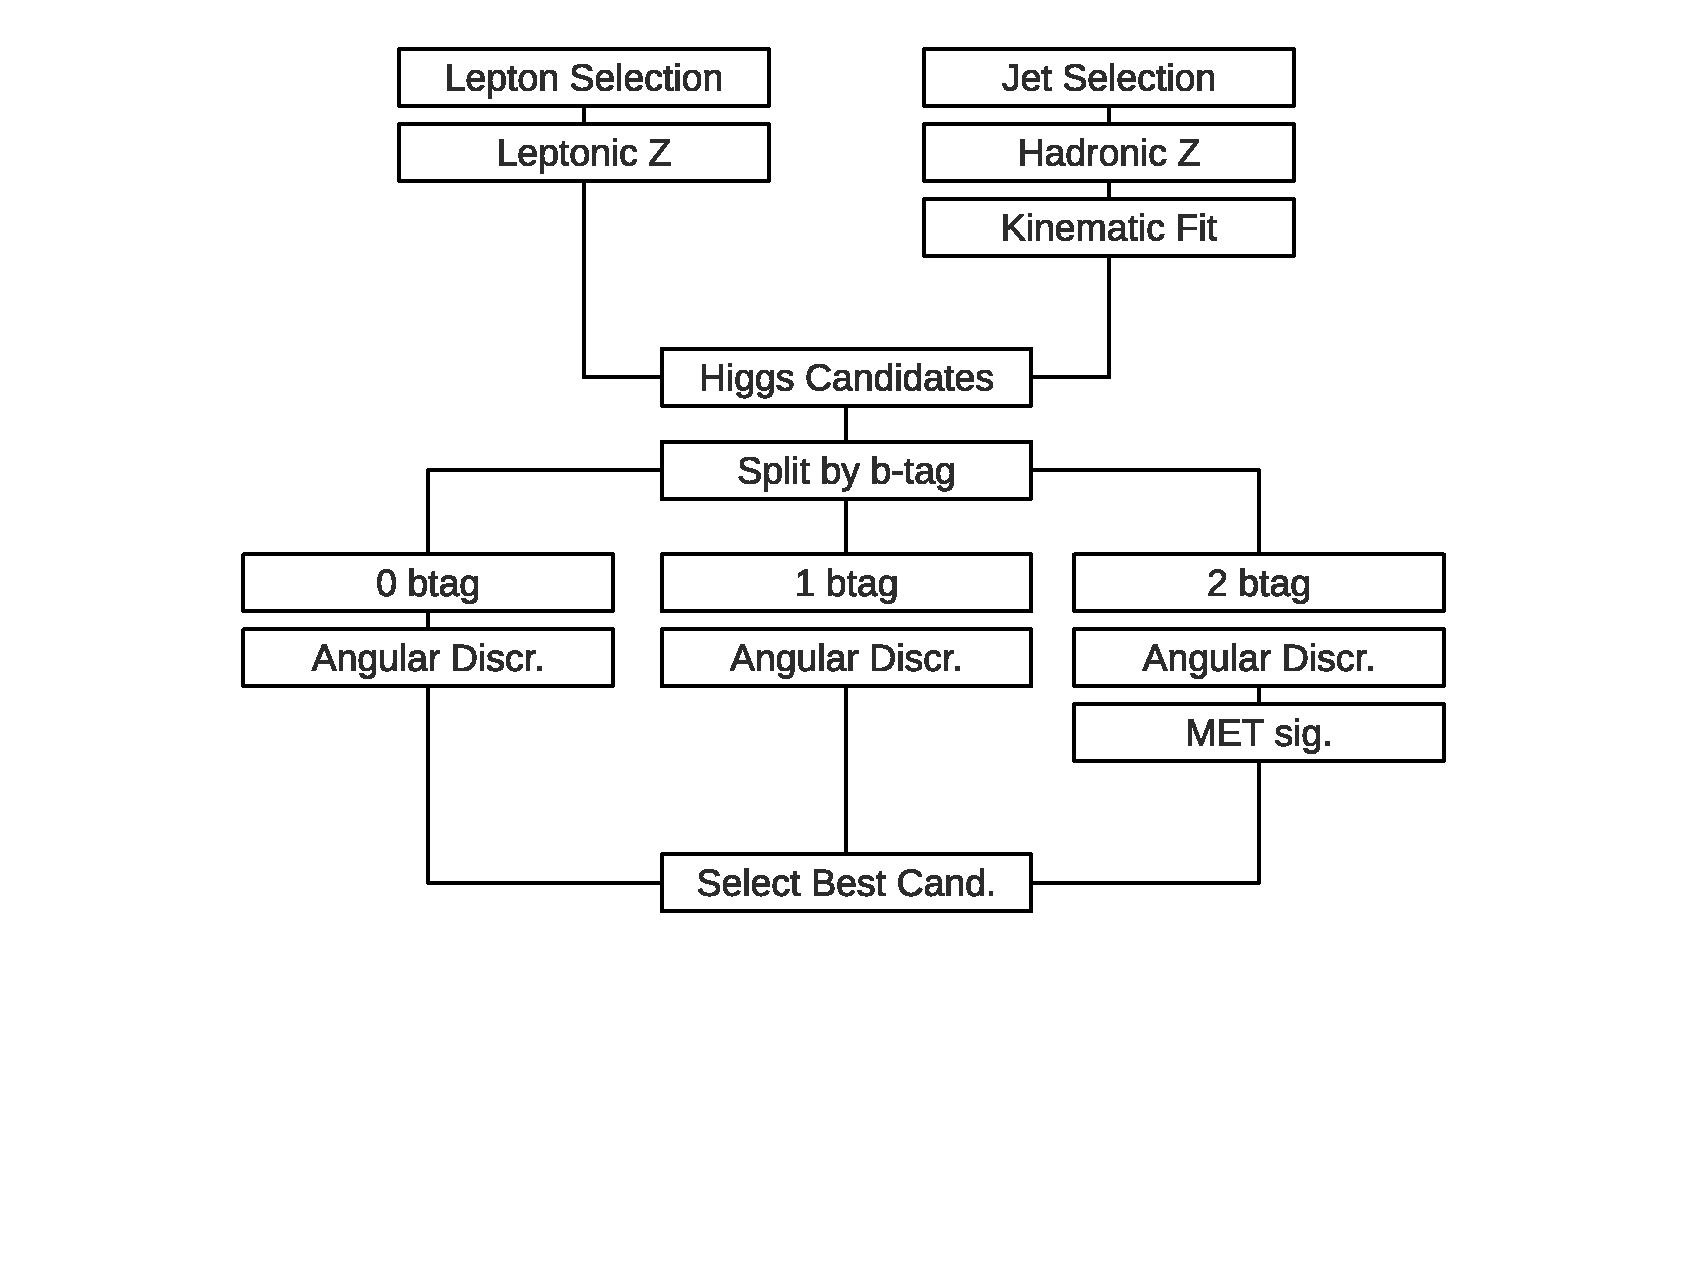
\includegraphics[width=1.0\textwidth]{images/workflow.eps}
  \end{center}
\end{frame}


\begin{frame}{Samples}
%  \begin{itemize}
%  \item
%    Data is Double Electron and Double Muon datasets.
%  \item
%    Background Monte Carlo is primaraly Z+Jets make with the MADGRAPH.
%  \item
%    Other Backgrounds are TT, WW, WZ, ZZ with PYTHIA.
%  \item
%    The signal Monte Carlo samples are POWHEG.
%  \end{itemize}

\begin{center}

Data is Double Electron and Double Muon datasets.\\
\vspace{2em}
Background\\
\begin{tabular}{|c|c|c|}\hline
  MC Sample & Generator & Percent of Final Region \\ \hline \hline
  Z+Jets  & MADGRAPH & 80\% \\ \hline 
    tt      & PYTHIA & 7\%  \\ \hline
    ZZ      & PYTHIA & 11\% \\ \hline
    WZ      & PYTHIA & 2\%  \\ \hline
    WW      & PYTHIA & <1\% \\ \hline
\end{tabular}
\\
\vspace{2em}
The signal Monte Carlo samples are POWHEG.

$m_{H} = $200,210,220,230,250,275,300,325,\\
350,375,400,425,450,475,500,525,550,575,600 GeV

\end{center}

\end{frame}



\begin{frame}{Leptons}
  We are using the official prescriptions from the POGs for both Lepton ID and Isolation.
%\vspace{1em}
\begin{columns}
      \begin{column}{0.5\textwidth}
        \begin{center}
  {\bf Electrons}
  \begin{itemize}
    \footnotesize
  \item
    GSF Elecrons
  \item
    $p_{T}$ > 40/20 GeV, $|\eta|$ < 2.5
  \item
    Working Point Loose
  \item
    + Tight trigger cuts
  \item
    PU corrected ISO < 0.15
  \end{itemize}
  \vspace{2em}

  {\bf Muons}
  \begin{itemize}
    \footnotesize
    %\scriptsize
  \item
    reco::Muons
  \item
    $p_{T}$ > 40/20 GeV, $|\eta|$ < 2.4
  \item
    Tight Muon
  \item
    PU corrected ISO < 0.12
  \end{itemize}
  \end{center}
\end{column}
      
      \begin{column}{0.5\textwidth}
        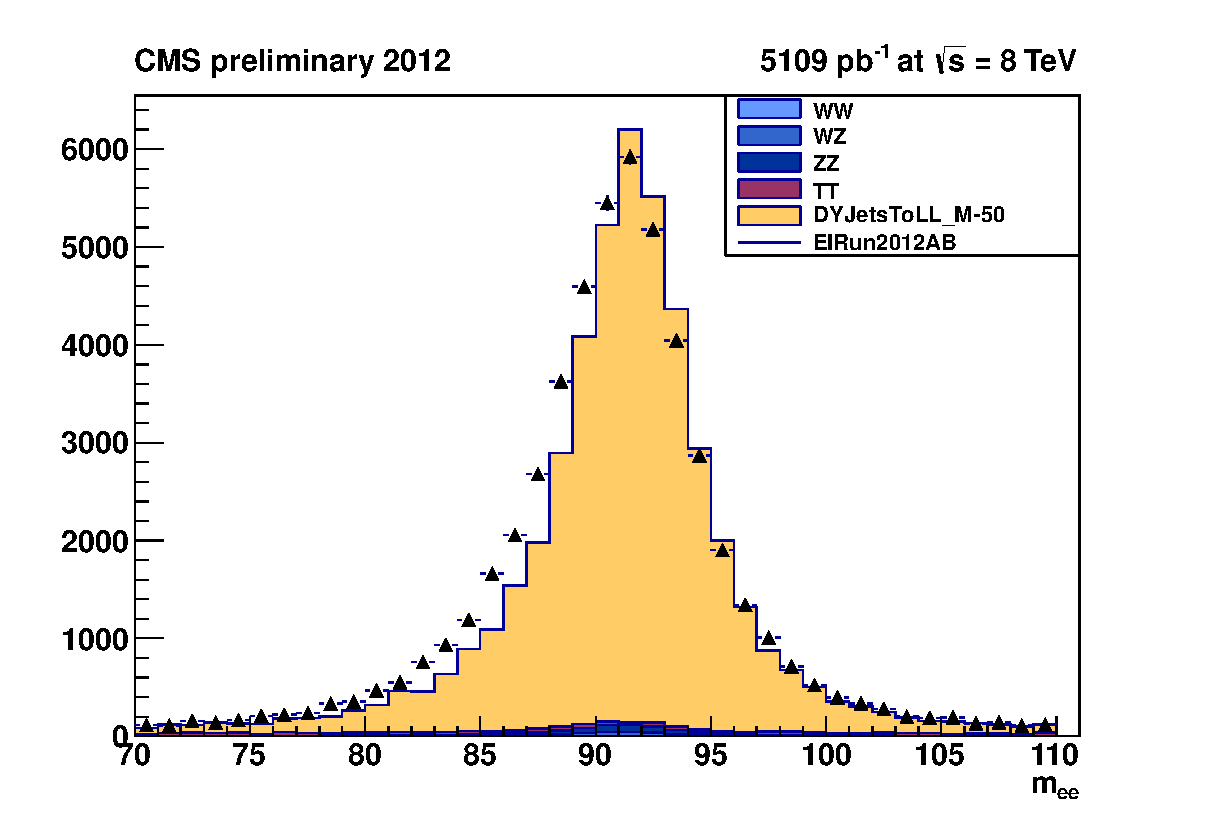
\includegraphics[width=0.8\textwidth]{images/stdCandle_ElRun2012.eps}\\
         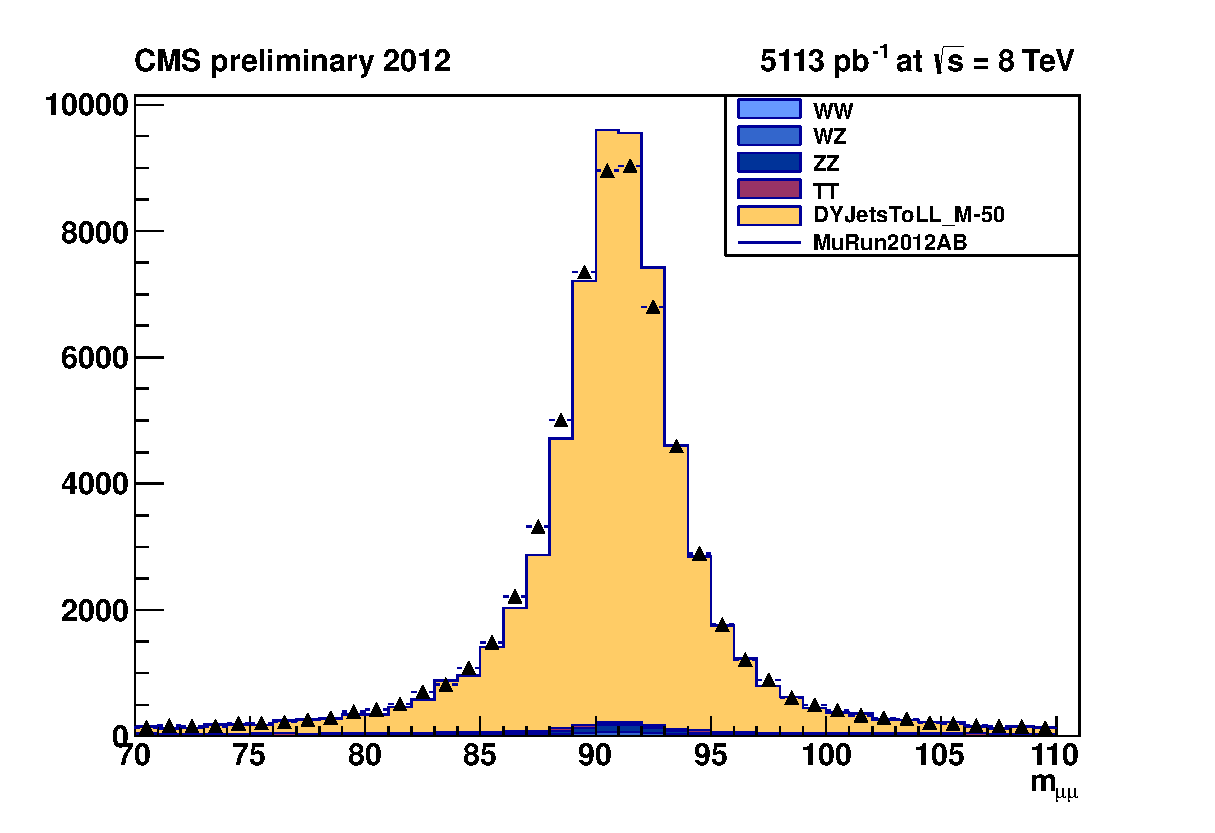
\includegraphics[width=0.8\textwidth]{images/stdCandle_MuRun2012.eps}
\end{column}
\end{columns}
\end{frame}




\begin{frame}{Jets}
  
      \begin{itemize}
      \item
        AK5PF, L1FastJet+L2+L3  %no MVA ID applied
      \item
        p$_{T}$ > 30 GeV , $|\eta|$ < 2.4
      \end{itemize}

  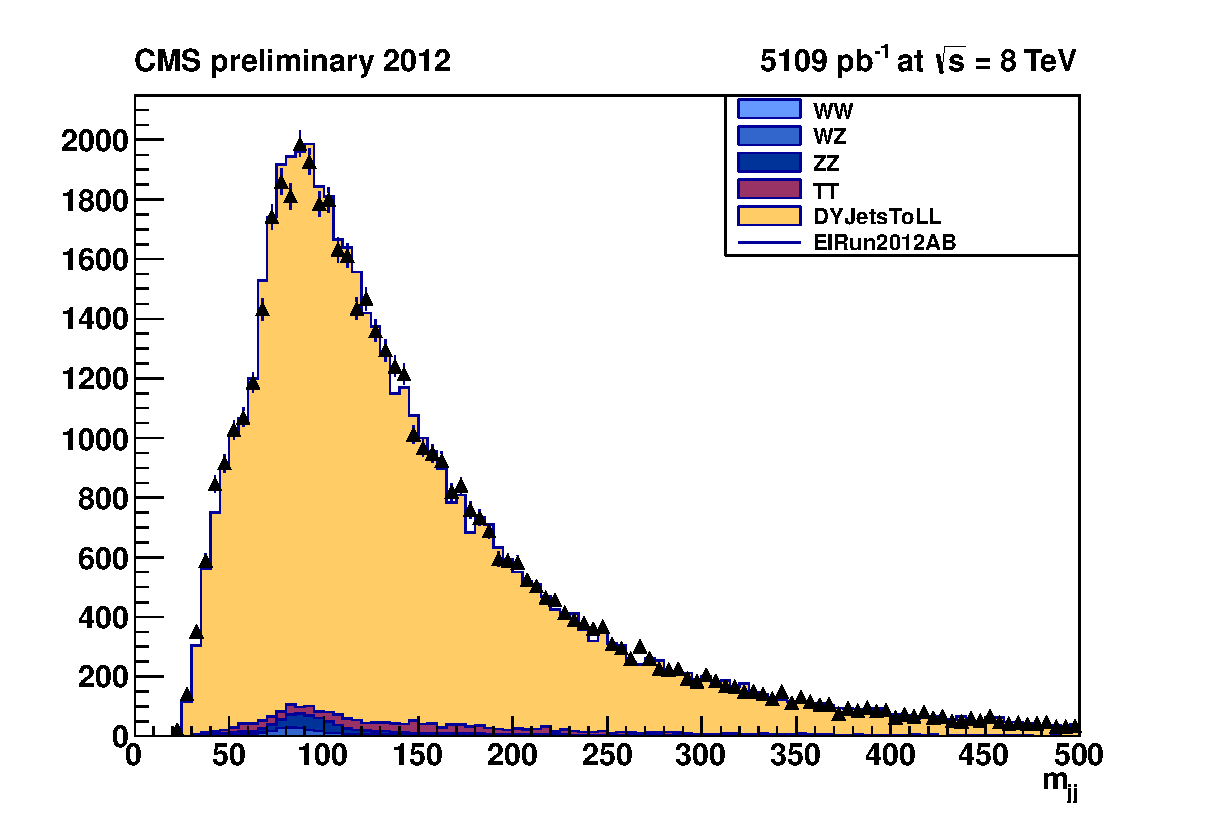
\includegraphics[width=0.5\textwidth]{images/zjjmass_ElRun2012.eps}
  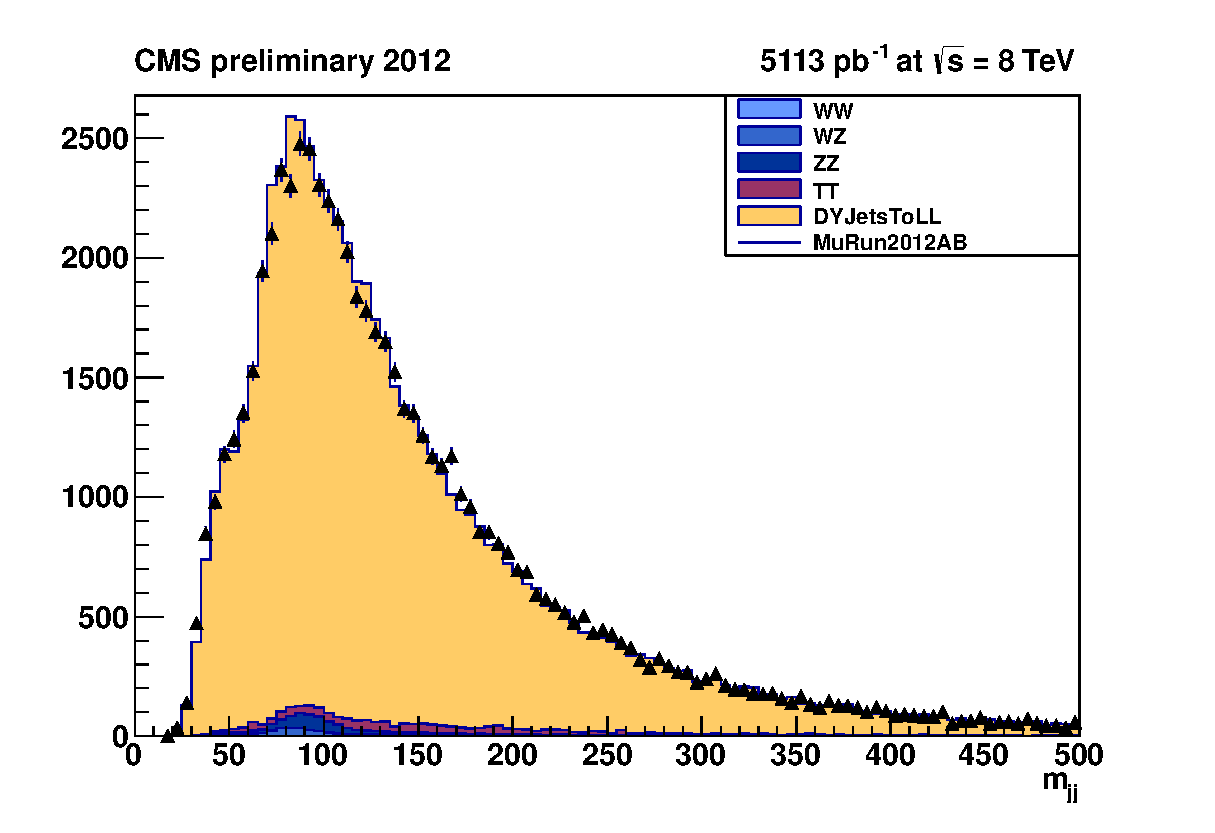
\includegraphics[width=0.5\textwidth]{images/zjjmass_MuRun2012.eps}

\end{frame}
















\begin{frame}{$b$-tagging}
  \begin{columns}
    \begin{column}{0.4\textwidth}
      \begin{itemize}
        {\small
        \item Using {\bf JP algorithm}, ``loose'' and ``medium'' WPs, allowing migrations among the tagging categories when applying the SF to MC
        \item Up to date using the latest calibrations available for the JP algorithm
        }
      \end{itemize}
      
    \end{column}
    
    \begin{column}{0.6\textwidth}
      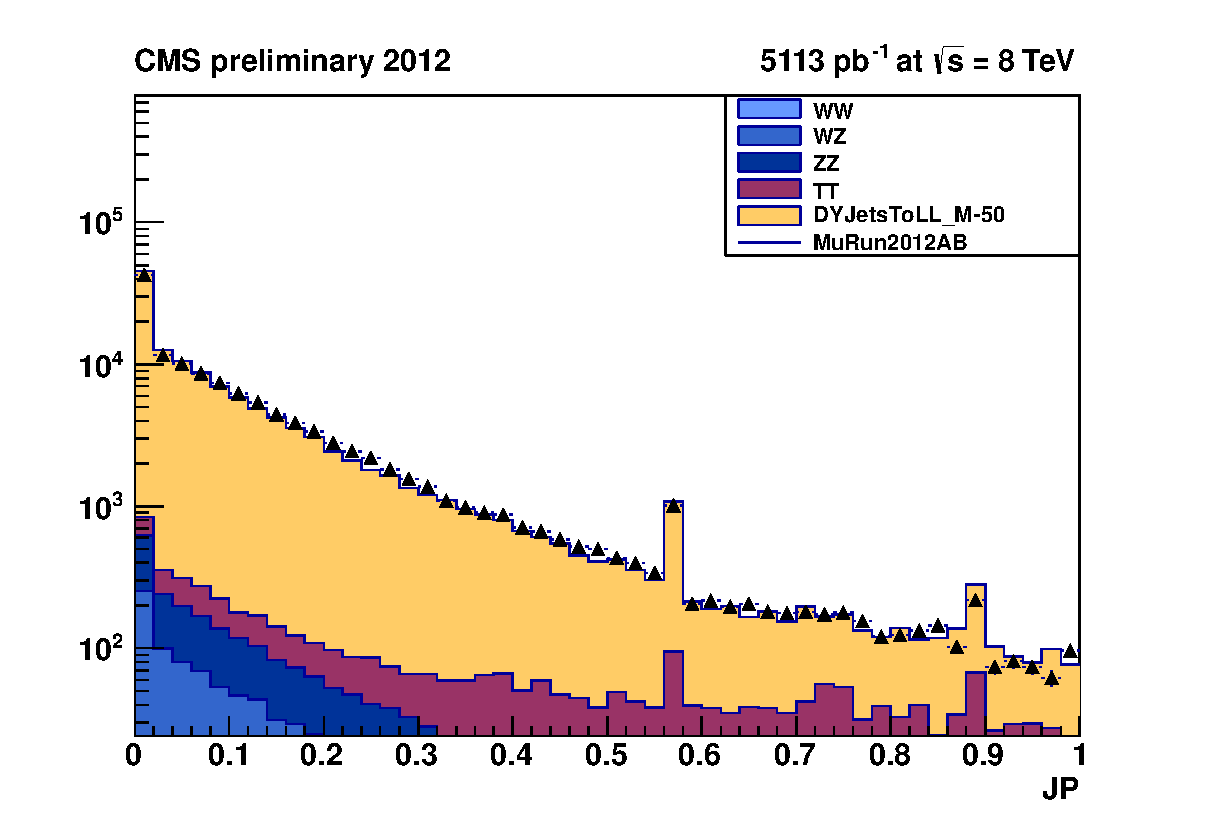
\includegraphics[width=0.99\textwidth]{images/JPJet_MuRun2012_LOG.eps}
    \end{column}
  \end{columns}
 \begin{center}
  \begin{tabular}{|c|c|}\hline
    0 - tag  & Both Jets < Loose \\ \hline 
    1 - tag  & > Loose and < Medium \\ \hline
    2 - tag  & > Loose and > Medium \\ \hline
  \end{tabular}
  \end{center}
\end{frame}



\begin{frame}{Signal and Sideband Regions}
  {\bf Study Regions}
  \begin{itemize}
  \item 
   Signal Region is 70 < m$_{ll}$ < 110 GeV and 75 < m$_{jj}$ < 105 GeV
  \item 
    Also we are looking at the sidebands region, defined as 60< m$_{jj}$ <75 GeV || 105< m$_{jj}$ <130 GeV (i.e. outside signal window 75< mjj < 105 GeV).
  \end{itemize}
 % 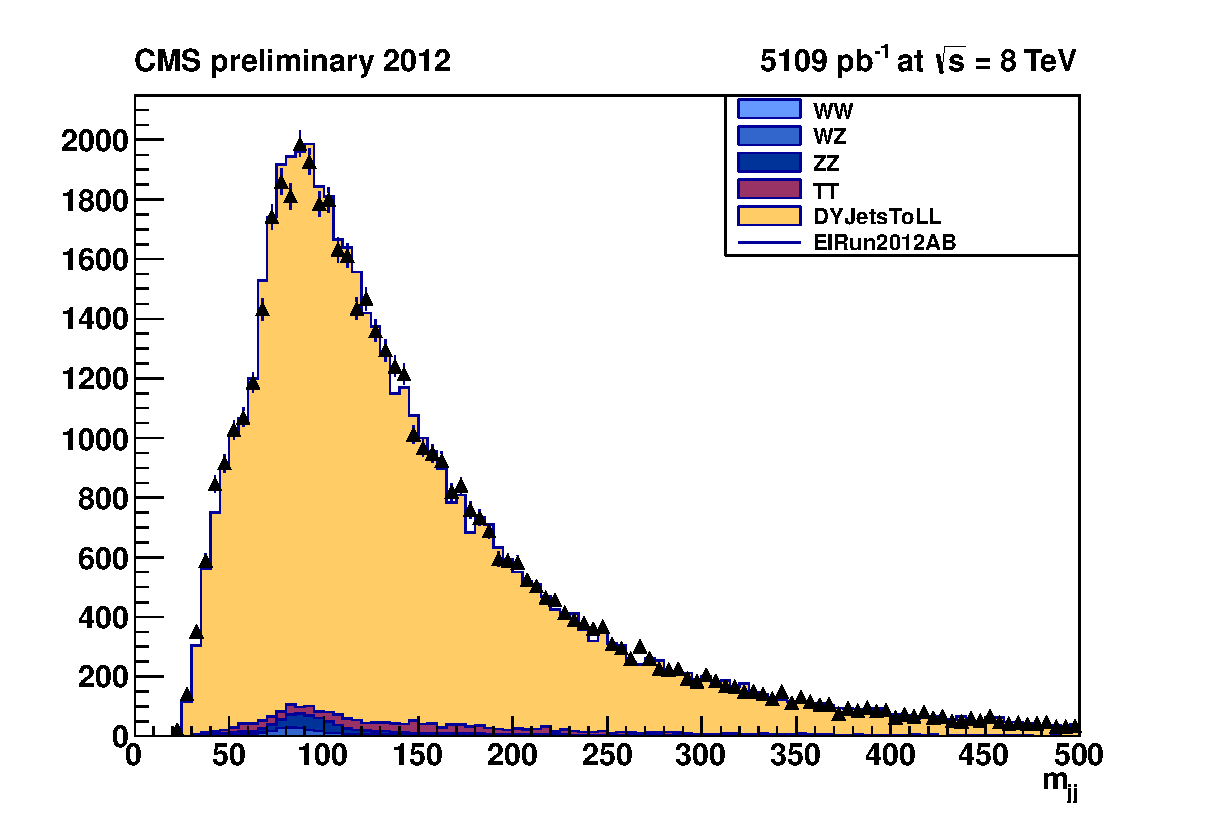
\includegraphics[width=0.5\textwidth]{images/zjjmass_ElRun2012.eps}
 % 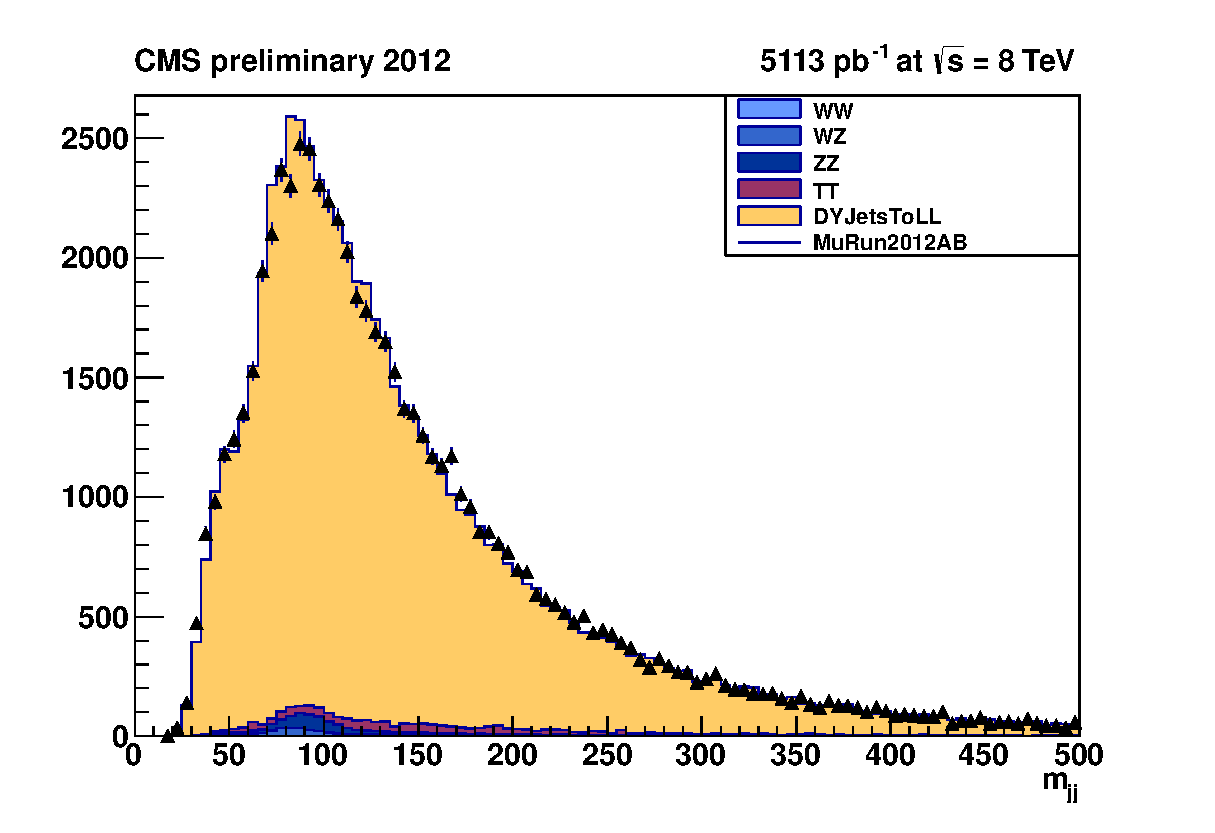
\includegraphics[width=0.5\textwidth]{images/zjjmass_MuRun2012.eps}
  \begin{center}
    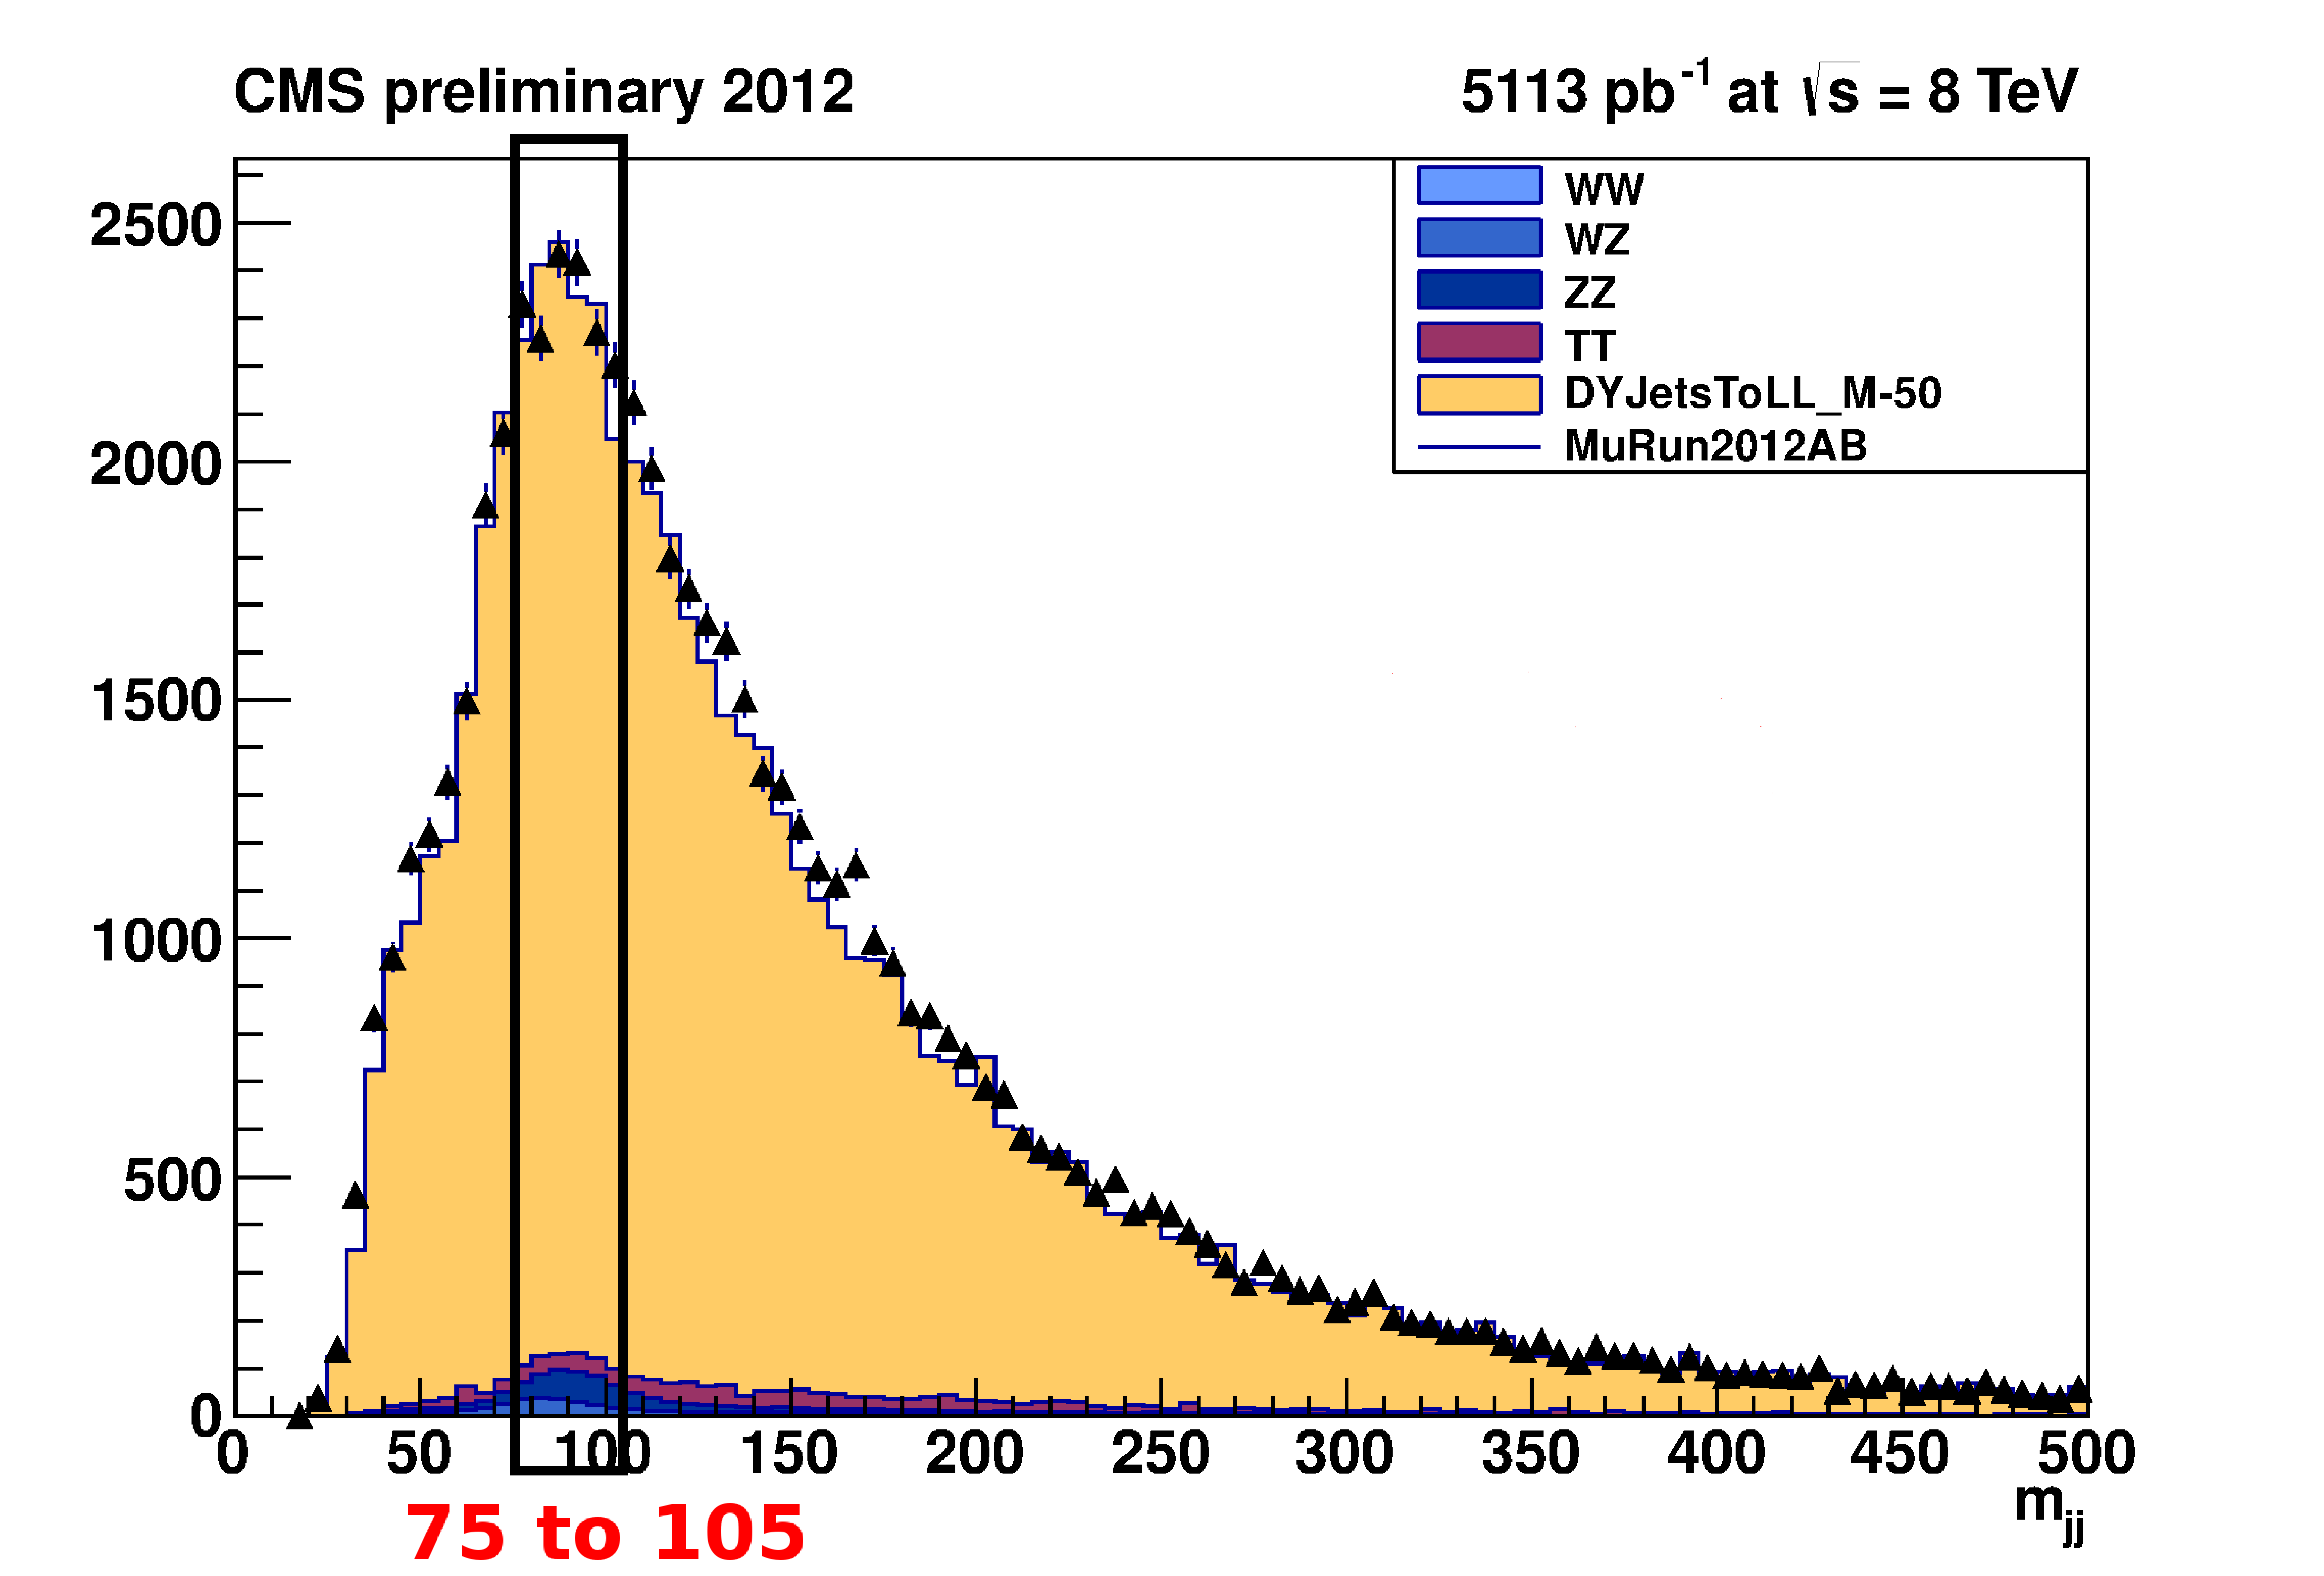
\includegraphics[width=0.6\textwidth]{images/zjjmass_MuRun2012_blind.eps}
  \end{center}

 % \begin{columns}
 %   \begin{column}{0.4\textwidth}
 %      \begin{block}{}
 %       \begin{center}
 %         All plots are either inclusive pre-selection or are in the sidebands.\\
 %        \end{center}
 %     \end{block}
 %   \end{column}
 %    \begin{column}{0.6\textwidth}
 %     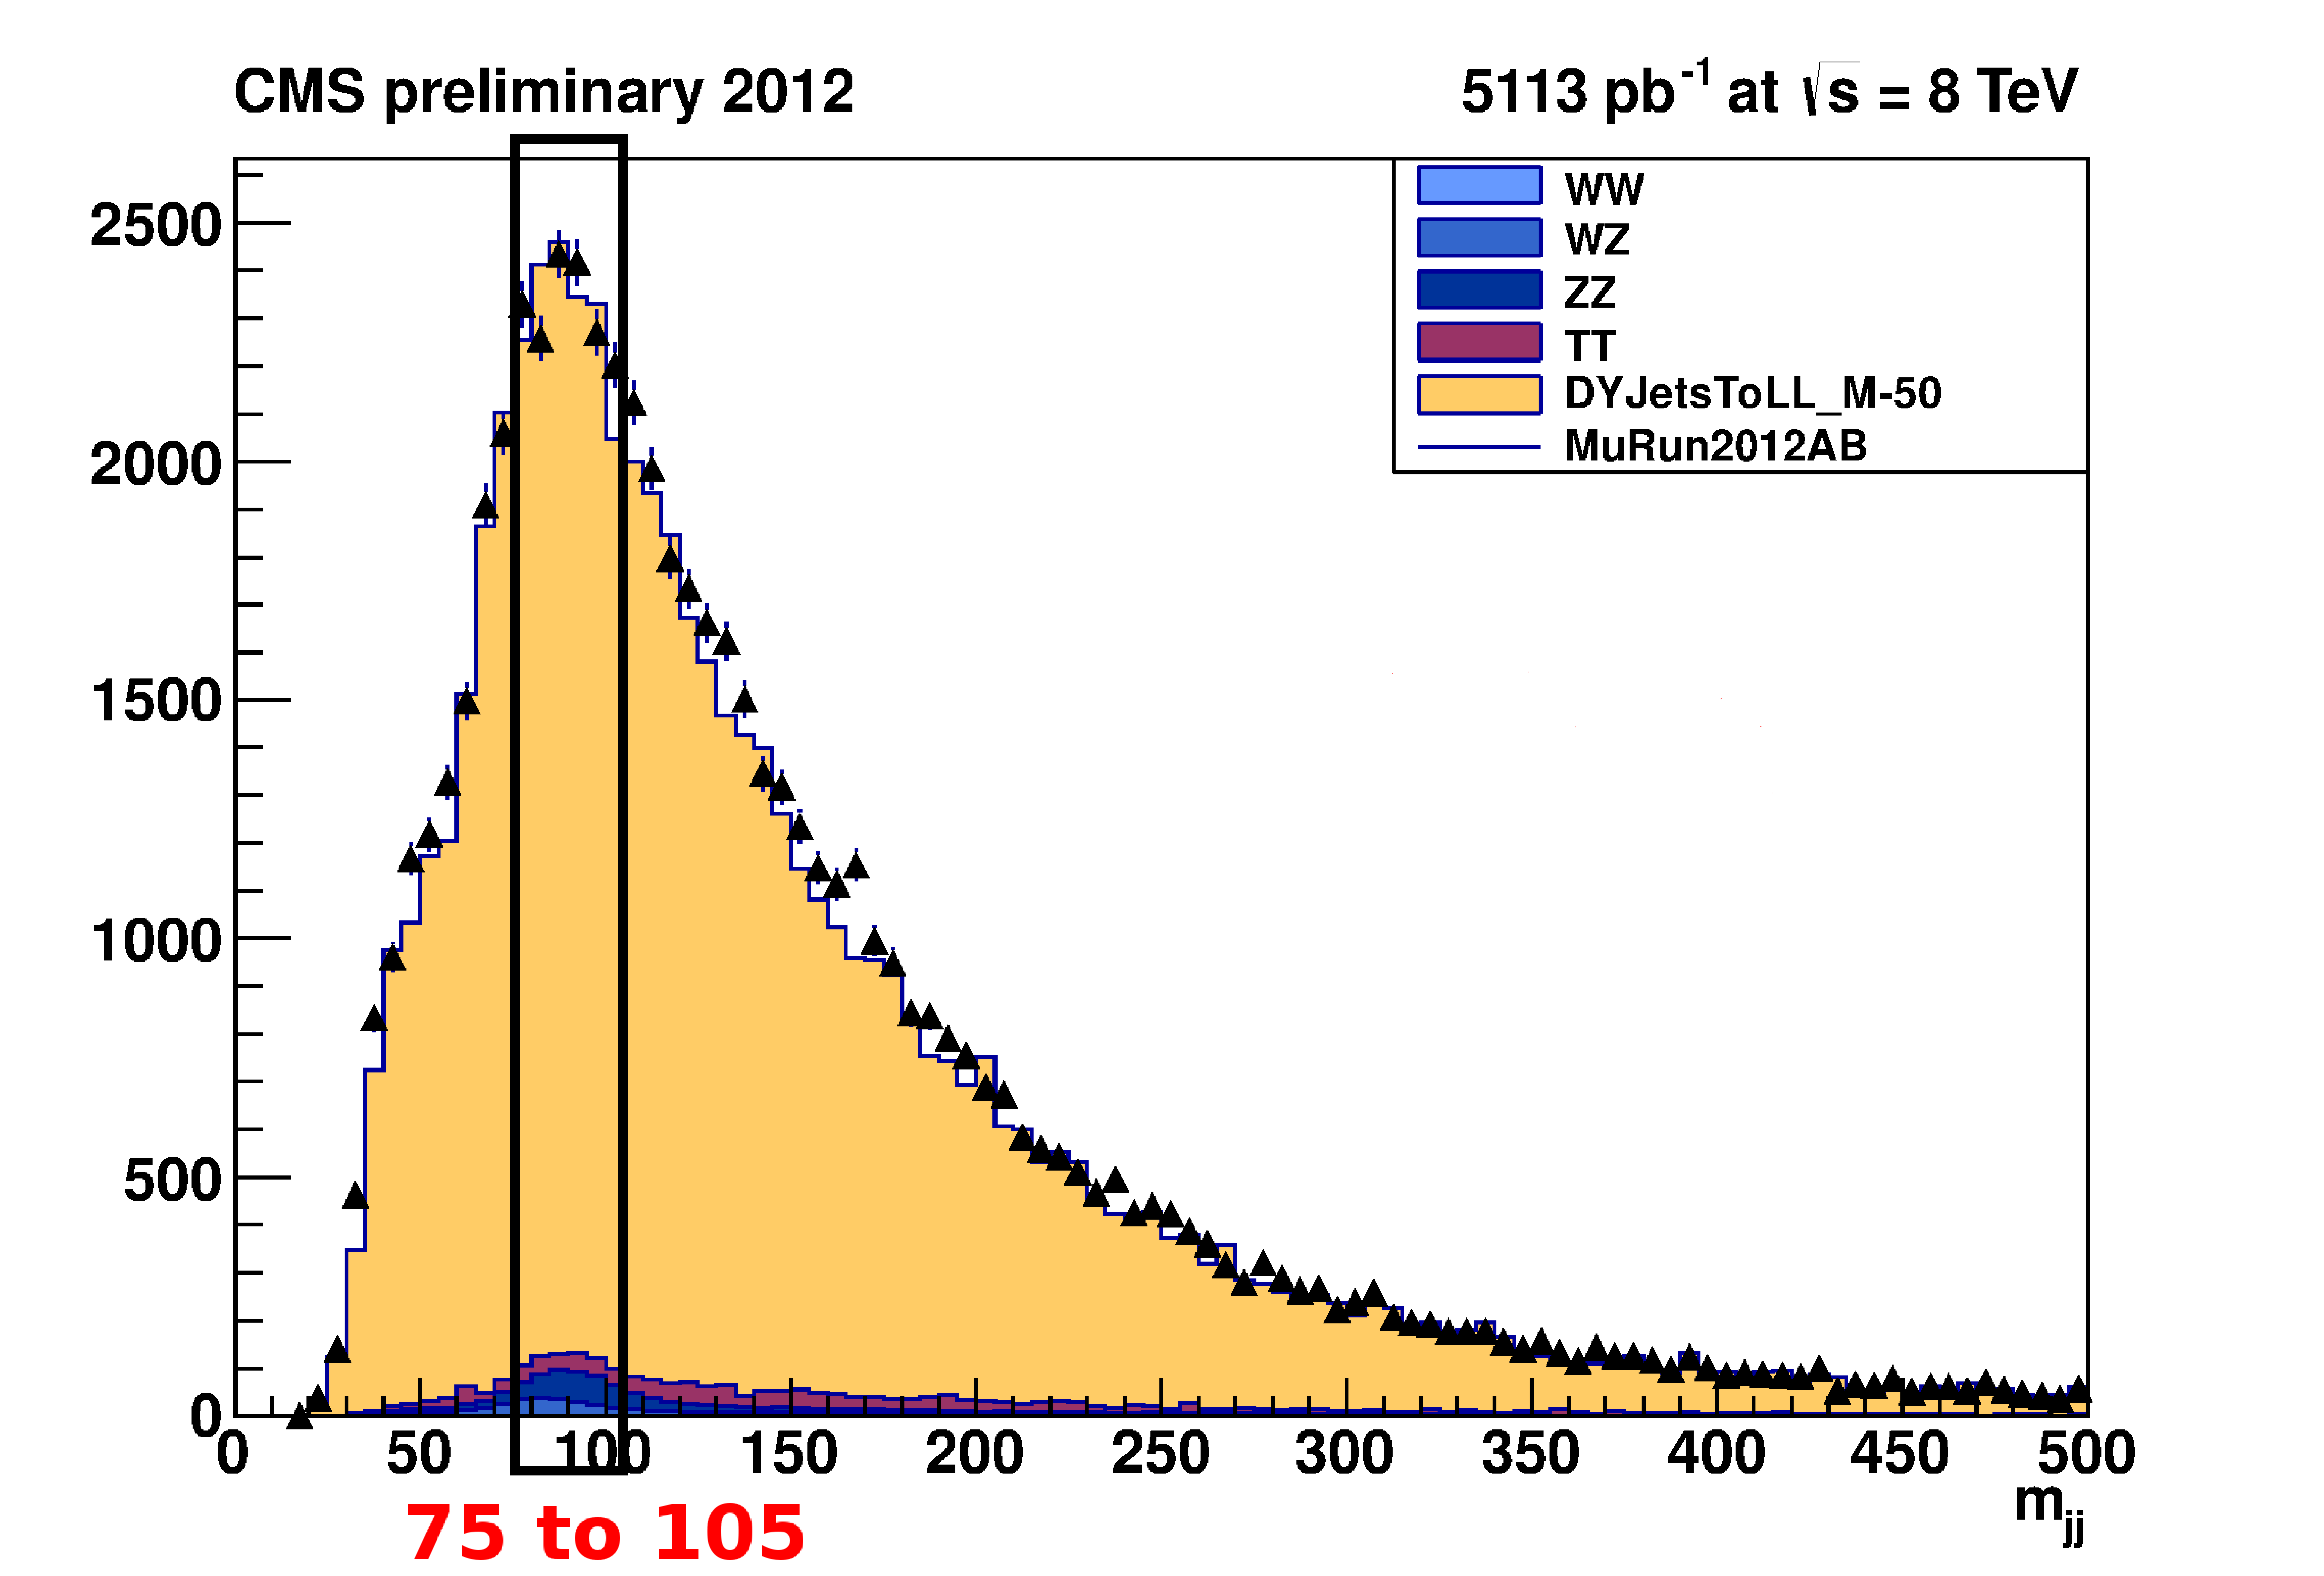
\includegraphics[width=0.9\textwidth]{images/zjjmass_MuRun2012_blind.eps}
 %    \end{column}
 % \end{columns}
  
\end{frame}

%\begin{frame}{Data-MC plots Pretag}
%  \begin{center}
%    Electrons\\
%    $\phi$ \hspace{7.5em} $\phi^{*}$ \hspace{7.5em} Helicity LD
%    \\
%  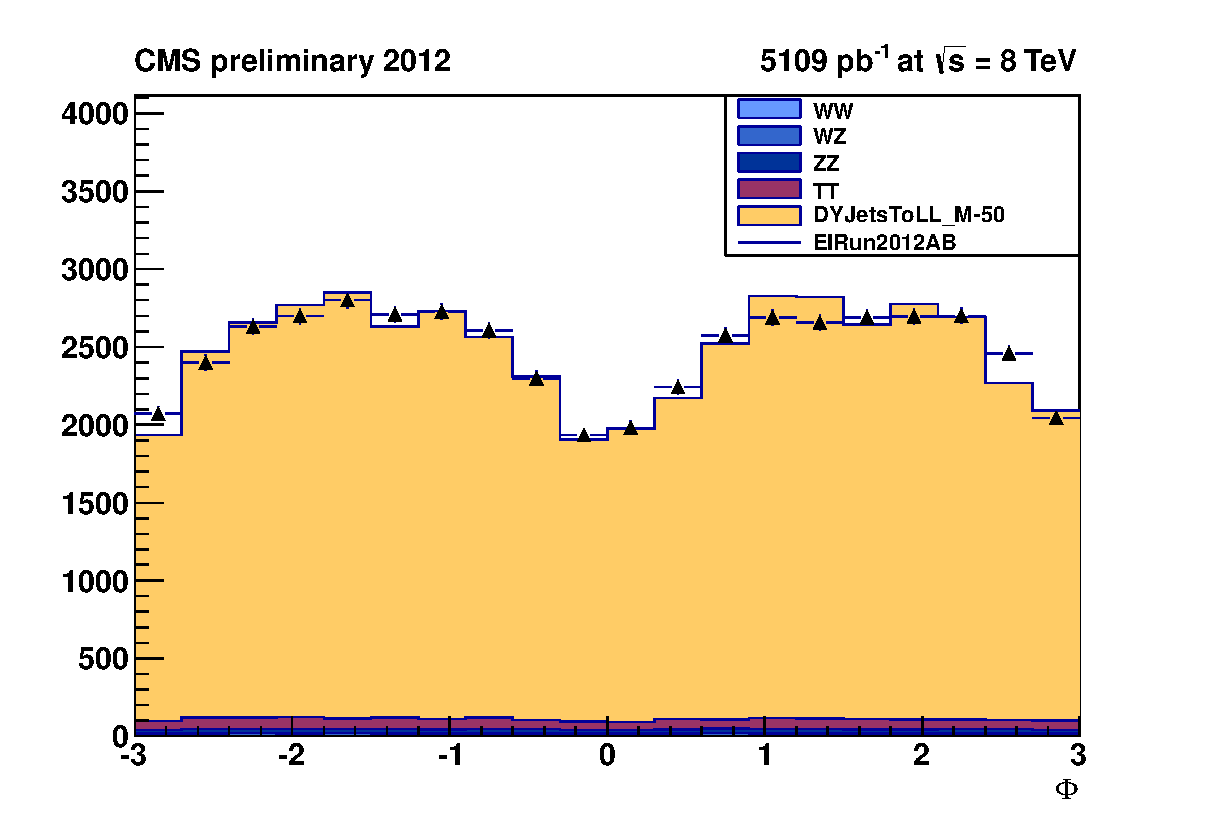
\includegraphics[width=0.33\textwidth]{images/phiRefit_ElRun2012.eps}
%  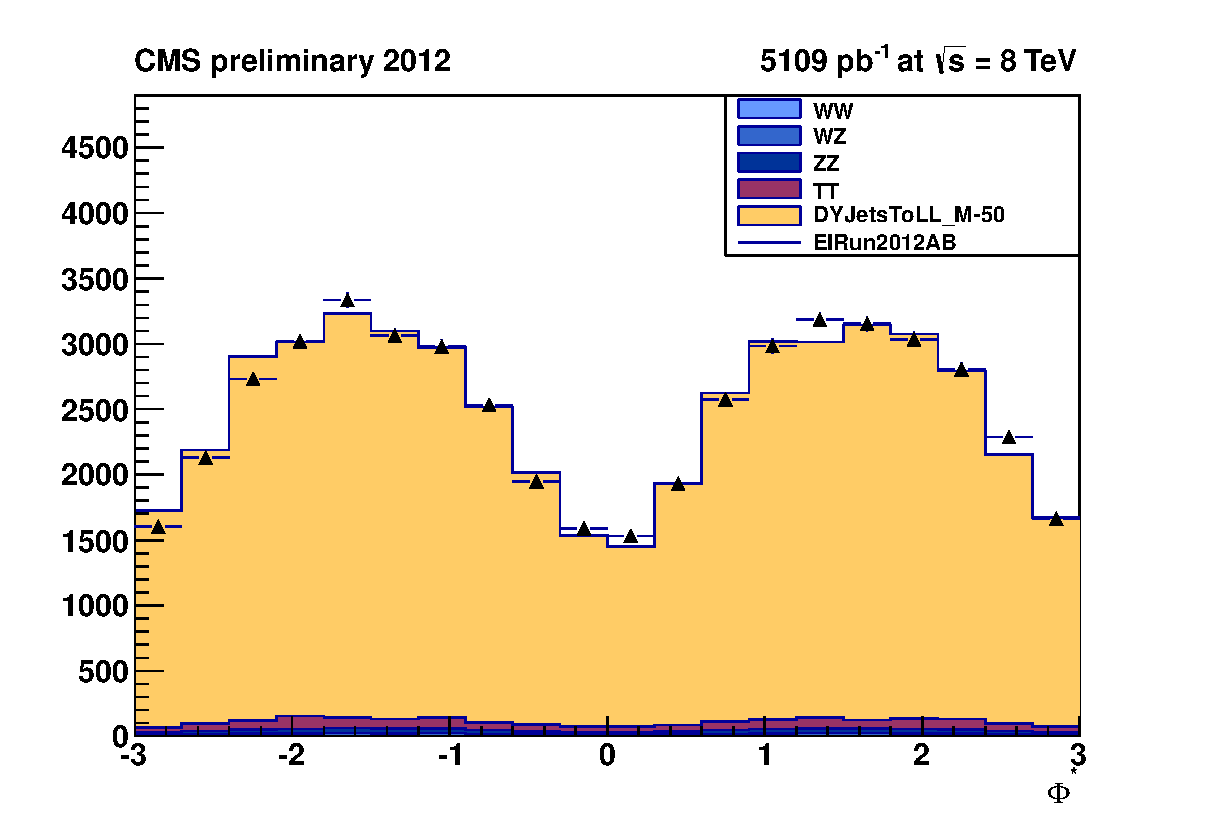
\includegraphics[width=0.33\textwidth]{images/phiStarRefit_ElRun2012.eps}
%  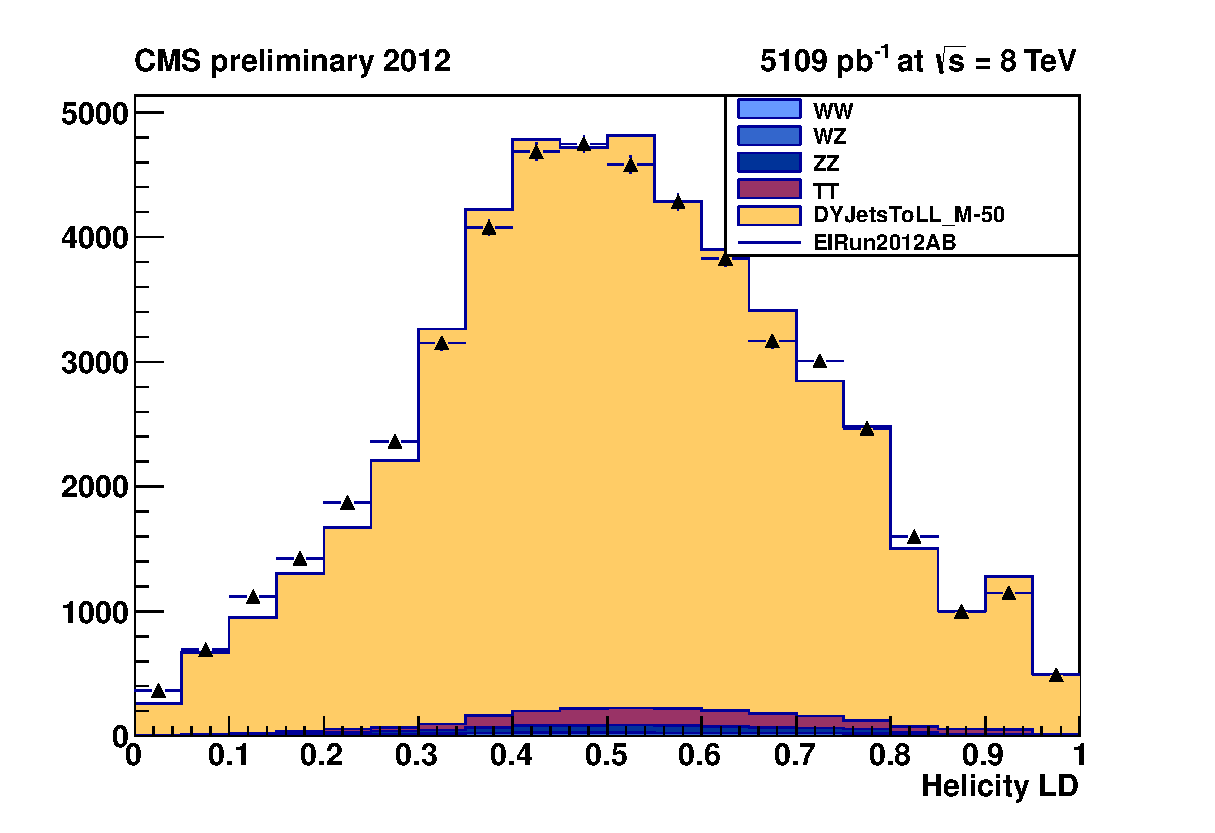
\includegraphics[width=0.33\textwidth]{images/HelyLDRefit_ElRun2012.eps}\\
%  $cos\theta_{1}$ \hspace{7.5em} $cos\theta_{1}^{*}$ \hspace{7.5em} $cos\theta_{2}$
%  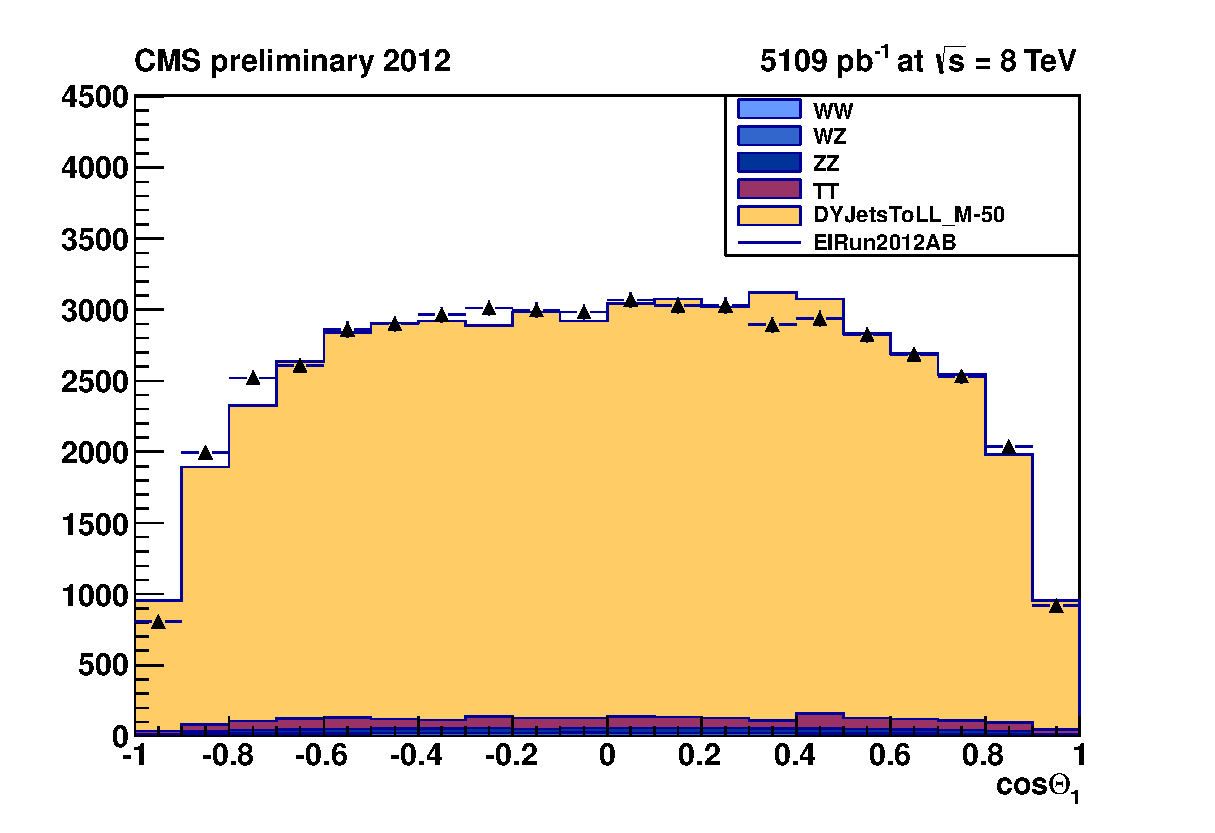
\includegraphics[width=0.33\textwidth]{images/cosTheta1Refit_ElRun2012.eps}
%  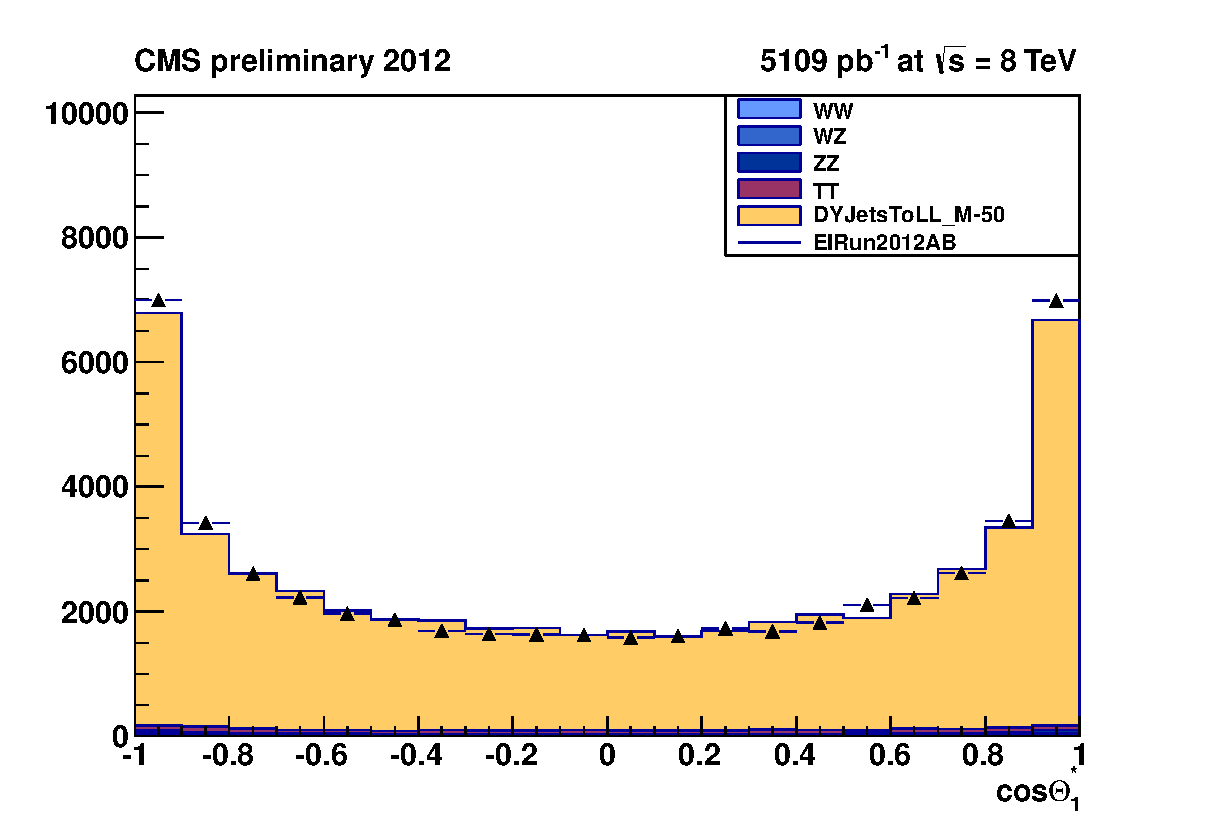
\includegraphics[width=0.33\textwidth]{images/cosTheta1StarRefit_ElRun2012.eps}
%  \includegraphics[width=0.33\textwidth]{images/cosTheta2Refit_ElRun2012.eps}
%  \end{center}
%\end{frame}



%\begin{frame}{Data-MC plots Pretag}
%  \begin{center}
%    Muons\\
%    $\phi$ \hspace{7.5em} $\phi^{*}$ \hspace{7.5em} Helicity LD
%    \\
%  \includegraphics[width=0.33\textwidth]{images/phiRefit_MuRun2012.eps}
%  \includegraphics[width=0.33\textwidth]{images/phiStarRefit_MuRun2012.eps}
%  \includegraphics[width=0.33\textwidth]{images/HelyLDRefit_MuRun2012.eps}\\
%  $cos\theta_{1}$ \hspace{7.5em} $cos\theta_{1}^{*}$ \hspace{7.5em} $cos\theta_{2}$
%  \includegraphics[width=0.33\textwidth]{images/cosTheta1Refit_MuRun2012.eps}
%  \includegraphics[width=0.33\textwidth]{images/cosTheta1StarRefit_MuRun2012.eps}
%  \includegraphics[width=0.33\textwidth]{images/cosTheta2Refit_MuRun2012.eps}
%  \end{center}
%\end{frame}

\begin{frame}{Data-MC $m_{lljj}$ plots - Side Band Region}
  \begin{center}
    Electrons\\
    0-tag \hspace{7.5em} 1-tag \hspace{7.5em} 2-tag
  \includegraphics[width=0.33\textwidth]{images/lljjmass_0btagSB_ElRun2012_LOG.eps}
  \includegraphics[width=0.33\textwidth]{images/lljjmass_1btagSB_ElRun2012_LOG.eps}
  \includegraphics[width=0.33\textwidth]{images/lljjmass_2btagSB_ElRun2012_LOG.eps}\\
  Muons\\
    0-tag \hspace{7.5em} 1-tag \hspace{7.5em} 2-tag
  
  \includegraphics[width=0.33\textwidth]{images/lljjmass_0btagSB_MuRun2012_LOG.eps}
  \includegraphics[width=0.33\textwidth]{images/lljjmass_1btagSB_MuRun2012_LOG.eps}
  \includegraphics[width=0.33\textwidth]{images/lljjmass_2btagSB_MuRun2012_LOG.eps}
  \end{center}
\end{frame}

%\begin{frame}{$m_{zz}$ Distribution Lineshape Reweighting 2012}
%  \begin{itemize}
%  \item
%    We have the machinery running and are implementing the lineshape reweighting for the 2012 analysis
%  \end{itemize}

%\begin{center}
%  \includegraphics[width=0.7\textwidth]{images/mh600_parton_mother.eps}
%\end{center}
%\end{frame}



\begin{frame}{Background Estimation}
  \scriptsize
  \begin{itemize}
  \item
    We use the mjj sideband in data to get the normalization and a MC shape correction.

 % \begin{block}{}
 %   Number of background events in the signal region extrapolated from 
 % the side band region using the $\alpha(m_{ZZ})$ factor (as a function
 % of m$_{ZZ}$)
 % \begin{equation}
 %   N_{\rm bkg}(m_{ZZ})
 %   =N_{\rm sb}(m_{ZZ})\times\frac{N^{\rm MC}_{\rm bkg}(m_{ZZ})}{N^{\rm MC}_{\rm sb}(m_{ZZ})}
 %   =N_{\rm sb}(m_{ZZ})\times\alpha(m_{ZZ})
 % \end{equation}
 %  \end{block}
\item
  The fit is to a Fermi*CrystallBall function
%  $\alpha$ is a flat factor while we wait for the exclusive samples
\end{itemize}

\begin{center}
%0-tag \vspace{7.5em} 1-tag \vspace{7.5em} 2-tag\\
    \includegraphics[width=0.3\textwidth]{images/fromDani/mZZ_sidebandsDATA_alpha_0btag_ALL_log.png}
    \includegraphics[width=0.3\textwidth]{images/fromDani/mZZ_sidebandsDATA_alpha_1btag_ALL_log.png}
    \includegraphics[width=0.3\textwidth]{images/fromDani/mZZ_sidebandsDATA_alpha_2btag_ALL_log.png}\\
0-tag \hspace{10.5em} 1-tag \hspace{10.5em} 2-tag
\end{center}

\end{frame}


\section{Signal Region Optimization}


\begin{frame}{Helicity and Production Angles}
\begin{center}
Final state kinematics completely determined by 5 angles.
\includegraphics[width=0.6\textwidth]{images/plots/angles-HZZ2l2q}
\\
$ cos(\theta^*), cos(\theta_1), cos(\theta_2), \Phi, \Phi_1$
\end{center}
\end{frame}


\begin{frame}{Electron Helicity and Production Angles}
\begin{center}
\includegraphics[width=0.33\textwidth]{images/plots/cosTheta1Refit_ElRun2012.png}
\includegraphics[width=0.33\textwidth]{images/plots/cosTheta2Refit_ElRun2012.png}
\includegraphics[width=0.33\textwidth]{images/plots/cosTheta1StarRefit_ElRun2012.png}
\\
\includegraphics[width=0.33\textwidth]{images/plots/phiStarRefit_ElRun2012.png}
\includegraphics[width=0.33\textwidth]{images/plots/phiRefit_ElRun2012.png}
%\includegraphics[width=0.33\textwidth]{images/plots/HelyLDRefit_ElRun2012.png}
\end{center}
\end{frame}


\begin{frame}{Muon Helicity and Production Angles}
\begin{center}
\includegraphics[width=0.33\textwidth]{images/plots/cosTheta1Refit_MuRun2012.png}
\includegraphics[width=0.33\textwidth]{images/plots/cosTheta2Refit_MuRun2012.png}
\includegraphics[width=0.33\textwidth]{images/plots/cosTheta1StarRefit_MuRun2012.png}
\\
\includegraphics[width=0.33\textwidth]{images/plots/phiStarRefit_MuRun2012.png}
\includegraphics[width=0.33\textwidth]{images/plots/phiRefit_MuRun2012.png}

\end{center}
\end{frame}



\begin{frame}{Angular Distribution Fits}
\begin{center}
Example fits at for 500 GeV (475 - 550 GeV).
\includegraphics[width=0.33\textwidth]{images/plots/sigPDF_CosTheta1proj_500.pdf}
\includegraphics[width=0.33\textwidth]{images/plots/sigPDF_CosTheta2proj_500.pdf}
\includegraphics[width=0.33\textwidth]{images/plots/sigPDF_CosThetaSproj_500.pdf}
\\
\includegraphics[width=0.33\textwidth]{images/plots/sigPDF_Phiproj_500.pdf}
\includegraphics[width=0.33\textwidth]{images/plots/sigPDF_PhiStar1proj_500.pdf}

%sigPDF_CosTheta1proj_500.pdf  sigPDF_CosTheta2proj_500.pdf  sigPDF_CosThetaSproj_500.pdf  sigPDF_Phiproj_500.pdf  sigPDF_PhiStar1proj_500.pdf

\end{center}
\end{frame}



\begin{frame}{Helicity LD}
\begin{center}
$LD = \dfrac{P_{sig}}{P_{sig} + P_{bkg}}$
\\
%\vpace{1em}
\includegraphics[width=0.5\textwidth]{images/plots/HelyLDRefit_ElRun2012.png}
\includegraphics[width=0.5\textwidth]{images/plots/HelyLDRefit_MuRun2012.png}
\\
\vspace{2em}
\tiny
\begin{tabular}{|l|c|c|c|}
\hline
 & 0 $b$-tag & 1 $b$-tag  & 2 $b$-tag \\
\hline
Helicity LD &  $>(0.55+0.00025\times m_{ZZ})$ & $>(0.302+0.000656\times m_{ZZ})$ & $> 0.5$ \\
%\vspace{-0.2cm}
%Quark-Gluon LD &  $>0.10$ & -- & --  \\
%\vspace{-0.2cm}
%\vspace{-0.2cm}
\hline
\end{tabular}
\end{center}
\end{frame}



\begin{frame}{Neural Network with TMVA Package}
\begin{center}
\includegraphics[width=0.8\linewidth]{images/plots/NN/nn_network_architecture}
\end{center}
\end{frame}



\begin{frame}{Neural Network Training and Testing}
\begin{center}
The trainings are done after preselection and additionally require at least one B-tagged Medium jet Left: Training 400 GeV Higgs boson with a MLP neural network.  Right: Training 400 GeV Higgs boson with a Likelihood.
\includegraphics[width=0.5\linewidth]{images/plots/NN/MLP_TCHEM.pdf}
\includegraphics[width=0.5\linewidth]{images/plots/NN/Likelihood_TCHEM.pdf}
\end{center}
\end{frame}


\begin{frame}{MLP vs Helicity LD}
\begin{center}
The working point is the background rejection point that we currently achieve in the two tag region in our analysis.
\includegraphics[width=0.7\linewidth]{images/plots/NN/pretag_ROC_wincut.pdf}
\end{center}
\end{frame}


\begin{frame}{High Mass MVA Introduction}
\begin{itemize}
\item
  Since the current helyLD optimization does not work at high mass I am looking at the performance of the straight forward MLP neural network performance in the High Mass region.
\item
  This looks at a training on the Higgs 400GeV signal sample (a trianing that works well for 300-600 as shown in previous talks) as well as the same training but on a Higgs 800 GeV signal sample.
\item
  These signal samples are the Gluon-Gluon samples
\end{itemize}
\end{frame}

%\begin{frame}{Optimization}
%\begin{itemize}
%  \item
%    Look at High Higgs mass (600,700,800,900,1000 GeV)
%  \item
%    Trained on 5 angular variables with signal of 400
%  \item
%    Previously shown similar results of helyLD with MLP NN for lower mass range (300,400,500,600)
%\end{itemize}
%\begin{center}
%Preselection    \hspace{7em}           Preselction + Higgs 400 mass cut
%\includegraphics[width=0.5\textwidth]{images/mva_highmass/full_hmass.eps}
%\includegraphics[width=0.5\textwidth]{images/mva_highmass/hmass.eps}\\
%  Twotag region Electrons (signal normalized to background)
%\end{center}
%\end{frame}

\begin{frame}{MLP}
\begin{center}
Electrons (zero,one,two)\\
\includegraphics[width=0.33\textwidth]{images/mva_highmass/zero_MLP.eps}
\includegraphics[width=0.33\textwidth]{images/mva_highmass/one_MLP.eps}
\includegraphics[width=0.33\textwidth]{images/mva_highmass/two_MLP.eps}\\
Muons (zero,one,two)\\
\includegraphics[width=0.33\textwidth]{images/mva_highmass/zero_mu_MLP.eps}
\includegraphics[width=0.33\textwidth]{images/mva_highmass/one_mu_MLP.eps}
\includegraphics[width=0.33\textwidth]{images/mva_highmass/two_mu_MLP.eps}\\
\end{center}
\end{frame}





\section{Cross Check and Statistical Analysis}


\begin{frame}{Neural Network with TMVA Package}
\begin{center}
\includegraphics[width=0.8\linewidth]{images/plots/NN/nn_network_architecture}
\end{center}
\end{frame}

\begin{frame}{Neural Network Training and Testing}
\begin{center}
The trainings are done after preselection and additionally require at least one B-tagged Medium jet. (Trained on H 400 GeV)
\includegraphics[width=0.7\linewidth]{images/plots/NN/MLP.eps}
%\includegraphics[width=0.5\linewidth]{images/plots/NN/Likelihood_TCHEM.pdf}
\end{center}
\end{frame}

%\begin{frame}{MLP}
%\begin{center}
%\includegraphics[width=0.49\textwidth]{images/preselection/el/MLP.eps}
%\includegraphics[width=0.49\textwidth]{images/preselection/mu/MLP.eps}\\
%\end{center}
%\end{frame}

\begin{frame}{MLP - In b-tag regions}
\begin{center}
Electrons (zero,one,two)\\
\includegraphics[width=0.33\textwidth]{images/preselection/0/el/MLP.eps}
\includegraphics[width=0.33\textwidth]{images/preselection/1/el/MLP.eps}
\includegraphics[width=0.33\textwidth]{images/preselection/2/el/MLP.eps}\\
Muons (zero,one,two)\\
\includegraphics[width=0.33\textwidth]{images/preselection/0/mu/MLP.eps}
\includegraphics[width=0.33\textwidth]{images/preselection/1/mu/MLP.eps}
\includegraphics[width=0.33\textwidth]{images/preselection/2/mu/MLP.eps}\\
\end{center}
\end{frame}

%\begin{frame}{MLP - Many Higgs Masses}
%\begin{center}
%Electrons (zero,one,two)\\
%\includegraphics[width=0.33\textwidth]{images/mva_highmass/zero_MLP.eps}
%\includegraphics[width=0.33\textwidth]{images/mva_highmass/one_MLP.eps}
%\includegraphics[width=0.33\textwidth]{images/mva_highmass/two_MLP.eps}\\
%Muons (zero,one,two)\\
%\includegraphics[width=0.33\textwidth]{images/mva_highmass/zero_mu_MLP.eps}
%\includegraphics[width=0.33\textwidth]{images/mva_highmass/one_mu_MLP.eps}
%\includegraphics[width=0.33\textwidth]{images/mva_highmass/two_mu_MLP.eps}\\
%\end{center}
%\end{frame}

\begin{frame}{MLP vs Helicity LD}
\begin{center}
The working point is the background rejection point that we currently achieve in the two tag region in our analysis.
\includegraphics[width=0.7\linewidth]{images/plots/NN/pretag_ROC_wincut.pdf}
\end{center}
\end{frame}









\begin{frame}{$m_{ZZ}$ plots - Side Band Region}
  \begin{center}
    Electrons\\
    0-tag \hspace{7.5em} 1-tag \hspace{7.5em} 2-tag
  \includegraphics[width=0.33\textwidth]{images/preselection/0/el/mZZ_sideband_log.eps}
  \includegraphics[width=0.33\textwidth]{images/preselection/1/el/mZZ_sideband_log.eps}
  \includegraphics[width=0.33\textwidth]{images/preselection/2/el/mZZ_sideband_log.eps}\\
  Muons\\
    0-tag \hspace{7.5em} 1-tag \hspace{7.5em} 2-tag
  
  \includegraphics[width=0.33\textwidth]{images/preselection/0/mu/mZZ_sideband_log.eps}
  \includegraphics[width=0.33\textwidth]{images/preselection/1/mu/mZZ_sideband_log.eps}
  \includegraphics[width=0.33\textwidth]{images/preselection/2/mu/mZZ_sideband_log.eps}
  \end{center}
\end{frame}


\begin{frame}{Upper vs Lower Sideband}
\begin{center}
  We also have very similar performance between the upper and lower sidebands in the $m_{ZZ}$ distribution so we are able to use them together.
  \includegraphics[width=0.5\textwidth]{images/sidebands/divide_el_2_0.eps}
   \includegraphics[width=0.5\textwidth]{images/sidebands/divide_mu_2_0.eps}
\end{center}
\end{frame}

\begin{frame}{Background Correction}
  \scriptsize
  \begin{itemize}
  \item
    We use the mjj sideband in data to get the normalization and a MC shape correction.

 % \begin{block}{}
 %   Number of background events in the signal region extrapolated from 
 % the side band region using the $\alpha(m_{ZZ})$ factor (as a function
 % of m$_{ZZ}$)
 % \begin{equation}
 %   N_{\rm bkg}(m_{ZZ})
 %   =N_{\rm sb}(m_{ZZ})\times\frac{N^{\rm MC}_{\rm bkg}(m_{ZZ})}{N^{\rm MC}_{\rm sb}(m_{ZZ})}
 %   =N_{\rm sb}(m_{ZZ})\times\alpha(m_{ZZ})
 % \end{equation}
 %  \end{block}
\item
  The fit is to a Fermi Function convoluted with a CrystallBall function
%  $\alpha$ is a flat factor while we wait for the exclusive samples
\end{itemize}

\begin{center}
%0-tag \vspace{7.5em} 1-tag \vspace{7.5em} 2-tag\\
    \includegraphics[width=0.3\textwidth]{images/fromDani/mZZ_sidebandsDATA_alpha_0btag_ALL_log.png}
    \includegraphics[width=0.3\textwidth]{images/fromDani/mZZ_sidebandsDATA_alpha_1btag_ALL_log.png}
    \includegraphics[width=0.3\textwidth]{images/fromDani/mZZ_sidebandsDATA_alpha_2btag_ALL_log.png}\\
0-tag \hspace{10.5em} 1-tag \hspace{10.5em} 2-tag
\end{center}

\end{frame}


%\begin{frame}{Selection Requirements}
%\begin{center}
%\begin{tabular}{|l|c|c|c|}
%\hline
% observable      &   0 $b$-tag   &   1 $b$-tag  &   2 $b$-tag  \\ \hline
%btag & none & JPL & JPL \& JPM \\ \hline
%helicity LD  &  \multicolumn{3}{|c|}{> 0.5}   \\ 
%missing $E_{T}$ significance &  \multicolumn{3}{|c|}{< 10}   \\ 
%$m_{jj}$  &  \multicolumn{3}{|c|}{[71,111] GeV/$c^{2}$}   \\ 
%$m_{ll}$  &  \multicolumn{3}{|c|}{[76,106] GeV/$c^{2}$}   \\ \hline
%$p_{T}(l^{\pm})$ & \multicolumn{3}{|c|}{> 40/20 GeV/c} \\
%$p_{T}(jets)$ & \multicolumn{3}{|c|}{> 30 GeV/c} \\
%|$\eta$|$(l^{\pm})$ & \multicolumn{3}{|c|}{$e^{\pm}$ < 2.5, $\mu^{\pm}$ < 2.4} \\
%|$\eta$|(jets) & \multicolumn{3}{|c|}{< 2.4} \\ \hline
%\multicolumn{4}{|c|}{lepton quailty} \\
%\multicolumn{4}{|c|}{jet quailty} \\ \hline
%\end{tabular}
%\end{center}
%\end{frame}


\begin{frame}{Tag and Probe}
\begin {itemize}
  \item
    Method to use Z boson to calculate efficincy of Data and Monte Carlo.
  \item
    One lepton is ``good'' (tag) and the other is used for the calculations(probe).
  \item
    Compairing Monte Carlo to data gives us Scale Factors.
\end{itemize}
\begin{center}
SuperCluster to GSF Electron\\
\includegraphics[width=0.49\textwidth]{images/SC_fit.eps}
\end{center}
\end{frame}


%\begin{frame}{Triggers}
%  \begin{columns}
%    \begin{column}{0.4\textwidth}
%      \begin{itemize}
%      \item
%        \footnotesize Muons
%        \begin{itemize}
%          \scriptsize
%        \item
%          HLT\_Mu17\_Mu8
%        \item
%          HLT\_Mu17\_TkMu8
%        \end{itemize}
%      \end{itemize}
%    \end{column}
%    \begin{column}{0.3\textwidth}
%      \begin{center}
%        {\tiny Electron Leg 8 GeV WPLoose to HLT}
%        \includegraphics[width=0.99\textwidth]{images/ZJets_8.eps}
%      \end{center}
%    \end{column}
%    \begin{column}{0.3\textwidth}
%      \begin{center}
%      {\tiny Electron Leg 17 GeV WPLoose to HLT}
%      \includegraphics[width=0.99\textwidth]{images/ZJets_17.eps}
%      \end{center}
%    \end{column}
%  \end{columns}
%  \begin{columns}
%    \begin{column}{1.0\textwidth}
%  \begin{itemize}
%  \item
%    \footnotesize  Electrons
%    \begin{itemize}
%      \tiny
%    \item
%      HLT\_Ele17\_CaloIdT\_CaloIsoVL\_TrkIdVL\_TrkIsoVL \_Ele8\_CaloIdT\_CaloIsoVL\_TrkIdVL\_TrkIsoVL
%    \end{itemize}
%  \item
%    \footnotesize EMu (for backround estimation and analysis checks)
%    \begin{itemize}
%      \scriptsize
%    \item
%      Mu8\_Ele17\_CaloIdT\_CaloIsoVL
%    \item
%      Mu17\_Ele8\_CaloIdT\_CaloIsoVL\_TrkIdVL\_TrkIsoVL
%    \end{itemize}
%  \end{itemize}
%  \end{column}
%    \begin{column}{0.0\textwidth}
%    \end{column}
%  \end{columns}
%\vspace{2em}
%We are using the POG provided scale factors for electrons and computing the WP to HLT ourselves. 
%\end{frame}














%\begin{frame}{Efficiency Fit}
%The signal efficiency as a function of the Higgs mass is fitted to a polynomial in order to be estimatated for those Higgs mass hypothesis where no Monte-Carlo sample is available
%\begin{center}
%\includegraphics[width=0.3\textwidth]{images/plots/effFit_MU_0btag.png}
%\includegraphics[width=0.3\textwidth]{images/plots/effFit_MU_1btag.png}
%\includegraphics[width=0.3\textwidth]{images/plots/effFit_MU_2btag.png}
%\\

%\includegraphics[width=0.3\textwidth]{images/plots/effFit_ELE_0btag.png}
%\includegraphics[width=0.3\textwidth]{images/plots/effFit_ELE_1btag.png}
%\includegraphics[width=0.3\textwidth]{images/plots/effFit_ELE_2btag.png}





%    Electrons\\
%    \includegraphics[width=0.3\textwidth]{images/fromDani/SignalEfficiencyFits27Sept_Run2012_AB/effFit_ELE_0btag.png}
%    \includegraphics[width=0.3\textwidth]{images/fromDani/SignalEfficiencyFits27Sept_Run2012_AB/effFit_ELE_1btag.png}
%    \includegraphics[width=0.3\textwidth]{images/fromDani/SignalEfficiencyFits27Sept_Run2012_AB/effFit_ELE_2btag.png}\\
%    Muons\\
%    \includegraphics[width=0.3\textwidth]{images/fromDani/SignalEfficiencyFits27Sept_Run2012_AB/effFit_MU_0btag.png}
%    \includegraphics[width=0.3\textwidth]{images/fromDani/SignalEfficiencyFits27Sept_Run2012_AB/effFit_MU_1btag.png}
%    \includegraphics[width=0.3\textwidth]{images/fromDani/SignalEfficiencyFits27Sept_Run2012_AB/effFit_MU_2btag.png}

%\end{center}
%\end{frame}




\begin{frame}{Signal Systematics}
\begin{center}
%\footnotesize
%\scriptsize
%\tiny

\begin{tabular}{|l|c|c|c|}
%\begin{tabular}{|l|c|c|c|p{5cm}|}
\hline
Source      &   0 $b$-tag   &   1 $b$-tag  &   2 $b$-tag   \\ \hline \hline
Muon trigger \& ID               &  \multicolumn{3}{c|}{2.7\%}       \\
Electron trigger \& ID           &  \multicolumn{3}{c|}{2\%}         \\ \hline
Electron energy scale            &  \multicolumn{3}{c|}{0.2\%}       \\
Muon momentum scale              &  \multicolumn{3}{c|}{0.1\%}       \\ \hline
Jet reconstruction               &  \multicolumn{3}{c|}{1-4\%}       \\ \hline
$b$-tagging eff. and mistag rate &  1-4\% & 1-5\% & 5-8\%             \\ \hline
MET                              &  \multicolumn{3}{c|}{$<1$\%}       \\ \hline
Pile-up                          &  \multicolumn{3}{c|}{1-2\%}        \\
Production mechanism (PDF)       &  \multicolumn{3}{c|}{1.5\%}       \\
Production mechanism (lineshape) &  \multicolumn{3}{c|}{0-3\%}       \\
Luminosity                       &  \multicolumn{3}{c|}{4.4$\%$}      \\
Higgs cross-section              &  \multicolumn{3}{c|}{13-15$\%$ }  \\
\hline
\end{tabular}

%\begin{tabular}{|l|c|c|c|l|}
%\hline
%Source      &   0 $b$-tag   &   1 $b$-tag  &   2 $b$-tag  &   Comment \\ \hline \hline
%Muon trigger \& ID               &  \multicolumn{3}{c|}{2.7\%}       & Tag-\&-probe study \\
%Electron trigger \& ID           &  \multicolumn{3}{c|}{2\%}         & Tag-\&-probe study  \\ \hline
%Electron energy scale            &  \multicolumn{3}{c|}{0.2\%}       & \\
%Muon momentum scale              &  \multicolumn{3}{c|}{0.1\%}       & \\ \hline
%Jet reconstruction               &  \multicolumn{3}{c|}{1-4\%}       & JES, correlated among categories \\ \hline
%$b$-tagging eff. and mistag rate &  1-4\% & 1-5\% & 5-8\%            & Anti-correlated among categories \\ \hline
%MET                              &  \multicolumn{3}{c|}{$<1$\%}      & Loose requirement \\ \hline
%Pile-up                          &  \multicolumn{3}{c|}{1-2\%}       & Correlated between categories \\
%Production mechanism (PDF)       &  \multicolumn{3}{c|}{1.5\%}       & PDF4LHC, acceptance only\\
%Production mechanism (lineshape) &  \multicolumn{3}{c|}{0-3\%}       & Only for $M_H>400 GeV$  \\
%Luminosity                       &  \multicolumn{3}{c|}{4.4$\%$}     & Same for all analyses \\
%Higgs cross-section              &  \multicolumn{3}{c|}{13-15$\%$ }  & CERN Yellow Report   \\
%\hline
%\end{tabular}






\end{center}
\end{frame}

\begin{frame}{Background Systematics}
\begin{center}
\footnotesize
\begin{tabular}{|l|c|c|c|c|c|c|}
\hline
                           &   \multicolumn{3}{c|}{Normalization}   &   \multicolumn{3}{c|}{Shape}  \\ \hline
Source &   0 $b$-tag   &   1 $b$-tag  &   2 $b$-tag &   0 $b$-tag   &   1 $b$-tag  &   2 $b$-tag \\ \hline \hline
Muon trigger \& ID               &  \multicolumn{3}{c|}{2.7\%}            &    \multicolumn{3}{c|}{}      \\
Muon momentum scale              &  \multicolumn{3}{c|}{0.1\%}            &    \multicolumn{3}{c|}{}      \\
Electron trigger \& ID           &  \multicolumn{3}{c|}{2.0\%}            &    \multicolumn{3}{c|}{}      \\
Electron energy scale            &  \multicolumn{3}{c|}{0.5\%}            &     \multicolumn{3}{c|}{}     \\
Jet energy scale                 &  \multicolumn{3}{c|}{5.5\%}            &  \multicolumn{3}{c|}{0-4\%}  \\ 
\hline
$b$-tagging efficiency SF        & +0.4\% & -0.8\%  & -4.5\% &           \multicolumn{3}{c|}{} \\
Mistag SF                        & -1.9\% & +7.8\% & +6.2\%             &      \multicolumn{3}{c|}{}    \\ 
\hline
MET                              &  \multicolumn{3}{c|}{0.3\%}            &     \multicolumn{3}{c|}{}     \\ 
Pile-up                          &  \multicolumn{3}{c|}{0.1\%}            &     \multicolumn{3}{c|}{}     \\
$\pt^{\ell\ell jj}$ weighting       &  \multicolumn{3}{c|}{0.8\%}            &   \multicolumn{3}{c|}{0-3\%}  \\
Diboson cross section            &  \multicolumn{3}{c|}{15\%}             &     \multicolumn{3}{c|}{}     \\
Luminosity                       &  \multicolumn{3}{c|}{4.4\%}           &      \multicolumn{3}{c|}{}    \\ \hline 
Control Region                   &    \multicolumn{3}{c|}{}               &  0-15\% &  0-30\% &  0-40\%  \\
\hline 
\end{tabular} 
\end{center}
\end{frame}



\section{Results}


\begin{frame}{8 TeV Results}
\begin{center}
\scriptsize
\begin{columns}
\begin{column}{0.6\textwidth}
\includegraphics[width=1.0\textwidth]{images/8TeV_limit.pdf}
\end{column}
\begin{column}{0.4\textwidth}
Observed (solid) and expected (dashed) 95\% CL upper limit on the ratio of the production cross section to the SM expectation for the Higgs boson obtained using the $\mathrm{CL_s}$ technique.\\
\vspace{1em}
The 68\% and 95\% ranges of expectation for the background-only model are also shown with green and yellow bands, respectively.  The solid line at 1 indicates the expectation for a SM-Higgs-like boson.
\end{column}
\end{columns}
\end{center}
\end{frame}

\begin{frame}{8 TeV Individual Channel Results}
\begin{center}
\includegraphics[width=0.33\textwidth]{images/limit_observed_0-btag_ee.pdf}
\includegraphics[width=0.33\textwidth]{images/limit_observed_1-btag_ee.pdf}
\includegraphics[width=0.33\textwidth]{images/limit_observed_2-btag_ee.pdf}\\
\includegraphics[width=0.33\textwidth]{images/limit_observed_0-btag_mm.pdf}
\includegraphics[width=0.33\textwidth]{images/limit_observed_1-btag_mm.pdf}
\includegraphics[width=0.33\textwidth]{images/limit_observed_2-btag_mm.pdf}\\
\end{center}
\end{frame}




\begin{frame}{HelyLD vs MLP}
\begin{center}
\scriptsize
%Limit on the expected 95$\%$ CL upper limit on the product of the Higgs boson production cross section and the branching fraction of H$\rightarrow$ZZ (dash line( and observed upper limit (black dots.) Yellow and Green bands represent the 68$\%$ and 95$\%$ ranges of expectation.
\begin{columns}
  \begin{column}{0.5\textwidth}
    \begin{center}
    {\large helyLD}\\ 
    \vspace{.2em}
   \includegraphics[width=1.\textwidth]{images/8TeV_limit.pdf}
   \end{center}
  \end{column}
  \begin{column}{0.5\textwidth}
    \begin{center}
    {\large MLP}\\
    \vspace{.2em}
    \includegraphics[width=1.\textwidth]{images/MVA_limit.pdf}
    \end{center}
  \end{column}
\end{columns}

\end{center}
%\vspace{.2em}
\footnotesize
The helyLD and MLP discriminators give very similar results, with the helyLD doing about 5\% better overall.  

\end{frame}




\begin{frame}{7 TeV and 8 TeV HelyLD Combined Results}
\begin{center}
\scriptsize
%Limit on the expected 95$\%$ CL upper limit on the product of the Higgs boson production cross section and the branching fraction of H$\rightarrow$ZZ (dash line( and observed upper limit (black dots.) Yellow and Green bands represent the 68$\%$ and 95$\%$ ranges of expectation.
\includegraphics[width=0.6\textwidth]{images/limit_observed_all-btag_combi.pdf}\\
\tiny
The 7 TeV 2l2q group results are in the backup slides.
\end{center}
\end{frame}



\section{Next Steps}

\begin{frame}{Next Step}
\begin{center}
%\scriptsize
\begin{itemize}
\item
  Train analysis for high mass range (from 600 GeV to 1000 GeV).
\item
  Run limit calculations on the MVA analysis.
\item
  Run tag and probe efficiency calculations for muons.
\item
  Optimize $Z_{ll}$ and $Z_{jj}$ cuts for preselection.
\item
  Improve reconstruction of high mass jets.
\item
  Run analysis over full 2012 data sample at the end of the run.
\end{itemize}


\end{center}
\end{frame}


\begin{frame}
\begin{center}
\huge
Thank You
\end{center}
\end{frame}


\section*{Backup}


\begin{frame}{Backup}

\begin{center}
BACKUP

\end{center}
\end{frame}

\begin{frame}{Pile-up Rejection}
\begin{center}
 $\beta$ is the sum of transverse momenta of all charged particles in the jet coming from the primary vertex, normalized to the total sum of transverse momenta of all charged particles in the jet.
 \begin{itemize}
  \item
    Using $\beta$ variable to remove candidates with PU-like jets 
  \item
    Cutting on $\beta \geq$~0.2
  \end{itemize}

\includegraphics[width=0.59\textwidth]{images/beta_MuRun2012.eps}
\end{center}
\end{frame}

\begin{frame}{$\dfrac{Signal}{\sqrt{Signal + Background}}$}
  
\begin{center}
400GeV Training
  \begin{tabular}{ | c | c | c | c | c | c | c |}
    \hline
    & \multicolumn{3}{|c|}{Electron} & \multicolumn{3}{|c|}{Muon}\\ \hline
    Sample  & zero& one  & two  & zero & one  & two  \\ \hline \hline
GG600 & 0.215 & 0.224 & 0.309 & 0.232 & 0.210 & 0.345\\ \hline
GG700 & 0.086 & 0.089 & 0.121 & 0.088 & 0.083 & 0.134\\ \hline
GG800 & 0.035 & 0.036 & 0.052 & 0.036 & 0.033 & 0.057\\ \hline
GG900 & 0.016 & 0.016 & 0.023 & 0.016 & 0.015 & 0.025\\ \hline
GG1000 & 0.009 & 0.009 & 0.012 & 0.009 & 0.008 & 0.013\\ \hline

\end{tabular}
\\
800GeV Training
\begin{tabular}{ | c | c | c | c | c | c | c |}
    \hline
    & \multicolumn{3}{|c|}{Electron} & \multicolumn{3}{|c|}{Muon}\\ \hline
    Sample  & zero& one  & two  & zero & one  & two  \\ \hline \hline
GG600 & 0.204 & 0.223 & 0.297 & 0.225 & 0.198 & 0.344\\ \hline
GG700 & 0.084 & 0.091 & 0.118 & 0.088 & 0.082 & 0.140\\ \hline
GG800 & 0.035 & 0.039 & 0.053 & 0.038 & 0.034 & 0.061\\ \hline
GG900 & 0.017 & 0.018 & 0.023 & 0.017 & 0.016 & 0.027\\ \hline
GG1000 & 0.009 & 0.009 & 0.012 & 0.009 & 0.009 & 0.014\\ \hline
\end{tabular}\end{center}
\end{frame}

\begin{frame}{Difference in $\dfrac{Signal}{\sqrt{Signal + Background}}$ 400 vs 800}
\begin{center}
  \begin{tabular}{ | c | c | c | c | c | c | c |}
    \hline
    & \multicolumn{3}{|c|}{Electron} & \multicolumn{3}{|c|}{Muon}\\ \hline
    Sample  & zero& one  & two  & zero & one  & two  \\ \hline \hline

GG600 & 4.93\% & 0.18\% & 4.17\% & 2.98\% & 5.49\% & 0.33\% \\ \hline
GG700 & 1.72\% & -2.75\% & 2.58\% & 0.36\% & 1.57\% & -3.91\% \\ \hline
GG800 & -1.71\% & -7.89\% & -2.51\% & -4.42\% & -2.47\% & -7.02\% \\ \hline
GG900 & -2.87\% & -8.16\% & 0.30\% & -5.16\% & -4.40\% & -8.41\% \\ \hline
GG1000 & -2.62\% & -8.38\% & -1.75\% & -4.26\% & -2.13\% & -10.91\% \\ \hline

\end{tabular}
\end{center}

\end{frame}



\end{document}


